\documentclass[paper=a4, twoside=false, fontsize=12pt, parskip=half,
                bibliography=totoc, listof=totoc]{scrbook}

% General packages
\usepackage{sourdough}

% Basic attributes
\author{Hendrik Kleinwächter}
\title{The Sourdough Framework}

\begin{document}
\input{cover/cover-translated}
\titlepage

\frontmatter
{%
\hypersetup{hidelinks}
\ifdefined\HCode\else\tableofcontents\fi
}

\chapter{Preface}%
\label{ch:Preface}

If there is one food Germany is known for, it is probably bread.
There are thousands of varieties in Germany,
and making it has been an integral part of our culture.

My bread journey began during childhood. My mother, being a parent
of 3, would always use Saturdays to bake a delicious loaf for the family.
It was a white fluffy sandwich bread, and she made it within one to two hour using store-bought yeast.
Being a bit more experienced, I~now realize it's
ideal to wait a little while before cutting into your bread, but back then,
we kids couldn't wait. Mom would cut for us a few slices straight from the oven, and we would
immediately proceed to pour butter or jam on each slice. Within minutes,
one kilogram of flour would be consumed. Bread became an integral part of my
weekly food.

I~was lucky that my parents could afford a yearly ski trip to
Alto Adige in northern Italy. In the small town called Valdaora, we
would try new restaurants every year, yet always end up in our favorite
pizza place. The pizzas there were incredible. The dough
alone was so tasty that we would order just the bread with a
bit of olive oil and salt.

Of course, my question would always be, ``Mom, can we make this at home, too, please?''
So over the years, we became friends with the owners and would receive
more and more clues as how to make the perfect pizza dough. There
are no secret ingredients inside. It's just flour, water, salt, and a bit of yeast.
How can such a simple combination of ingredients create such an incredibly delicious
pizza dough? My parents, being creatures of habit, would return every year with us,
and every year, my interest would grow. At home, Mom and I~attempted to replicate
the recipe. We tried baking on a stone and on a steel. We tried adding oil to the dough and herbs
to the pizza sauce. We fell into an endless cycle of experiments. However, we never managed
to get close to the experience we had while on vacation.

Some years passed, and I~eventually began my studies in the small German city of Göttingen.
For the first time, I~was faced with shopping for my own bread. It was never
on my mind to actually start baking it for myself. I~would just buy
a good loaf while shopping at the supermarket. My favorite variety
was a \emph{Schwarzbrot: Korn an Korn}. It’s a very dark and hearty rye bread
with added berries and sunflower seeds.

Being a little naïve, I'd never before examined the packaging of what I~was
buying. One day, that changed.  I~looked at the label and was shocked. The
seemingly
healthy bread consisted of so many other things aside from flour and water.
The black color was not coming from the flour, but from caramelized sugar.
The packaging stated it was a sourdough bread, but then why was there additional yeast?
I~thought that if it was really sourdough, it shouldn't require additional
yeast. I~soon
realized that something was wrong with the bread I~was buying.
I~proceeded to check the other supermarket breads, only to discover that they, too,
contained ingredients I'd never heard of. That was the day I~lost trust
in supermarket bread.

At home, I~decided to research the proper way to make bread, and much to my surprise,
I~learned that the recipes for making pizza and bread were actually quite similar, yet
there were also differences. For example, some recipes would call for fresh yeast, while
others would call for dry. Diving deep into various online forums and all their many
discussions, I~became even more confused.
I~tried using different flours and different brands, all in both organic and non-organic varieties.
I~realized then that I~knew nothing about making bread. Recipes would often contradict each other,
leaving me further confused. They seemed like little more than a collection of apparently random
steps to follow. The baking instructions and temperatures too were all
different\dots

Meanwhile, having completed my studies, I~started work as an engineer.
We engineers are faced with many challenges. The compiler or runtime is
always screaming at you with errors, and it's your job to figure out how to fix them.
It can take hours, sometimes days, just to fix a simple problem. If you want
to become a software engineer, you have to develop a certain ``never-give-up'' attitude.

When writing code, software engineers often need to use a set of pre-made routines. These routines have been
written by other engineers and can then be used to ship code faster.
This pre-written code is commonly known as \emph{a framework}. In many cases,
these frameworks are not built by a single person but by engineers from all around the world,
each of whom can help by improving and changing the source code. Frameworks have made many successful
businesses possible.
In most cases, frameworks do exactly what they claim they do. However,
sometimes you are faced with issues you don't understand. In \qty{99.95}{\percent}
of all software bugs, the developer is the issue. Sometimes, however, the framework has a
bug. That is when the developer must dig deeper to see the \emph{what} and the
\emph{why} behind what
the framework is doing. You will need to read other engineer's source code, and you will be forced
to understand \emph{why} things are happening.

Being unhappy with what I~was baking, my engineering mindset took over, and I~had
to do my own deep dive to understand what was going on. Much to my surprise, however,
none of the recipes I'd encountered would tell me \emph{why} I~should use amount X
of water and amount Y of flour, or \emph{why} exactly I~should use fresh yeast over dry yeast. Why
should I~slap my dough while kneading it on the counter? Why is a standmixer
better than kneading by hand? Why should I~let the dough sit for this long?
Why is steaming the dough during baking important? Do I~really need to
get myself an expensive Dutch oven to bake bread?
The problem compounded when I~started reading about sourdough. It all sounded like black
magic. Why were some sourdoughs made from fruits, while others were made from flour?
Why should one recipe use wheat while another used rye or spelt? How often should the
sourdough be fed? The questions I~had then could have filled 20~pages. I~was confused,
but I~became even more determined to learn how decent bread should be made at home.

The feedback I~received from friends helped me to improve with each
iteration of homemade bread. Compared to coding, where you sometimes have to wait months
for this feedback, bread making is much more direct. Plus, you can eat your successes
(and failures!) And, much to my surprise, even those failures started tasting better than
most store-bought breads. Eating a homemade bread that takes you hours to make allows you
to develop a different relationship with your food, and baking bread from scratch with my
bare hands was a welcome change after hours of working on the computer.

I~continued learning about the process of fermentation and various techniques of bread making.
I~approached the topic of sourdough in a manner similar to software, and after years of
researching and documenting my progress, I~decided it was time to share that progress with the
world.
When working on software projects, it is important to see their history and how the source
code changes over time. This way, you can easily jump back to previous versions. This was
the perfect tool for documenting my recipes, because they, too, would change with each
subsequent iteration. Much to my surprise, my open source work on sourdough was appreciated
by other engineers, and the project became popular on the website GitHub, originally built to
share open source software.

Now, when baking great bread, you also need to learn certain techniques. I~figured it would be
easier to share these techniques in video form. Thus, my YouTube channel was born. I~chose
the name \texttt{The Bread Code} to capture my engineering-oriented approach to bread. It took some
time to get it right, but after choosing more engaging thumbnails and titles for
the videos I~made, the channel started gaining viewers.
Finally, three years later, I~dedicate two days each week to follow my bread baking passion, while
the other three days I~continue to work as a software engineer, writing code on a day-to-day
basis.

My bread days fill me with both joy and passion. To me, there is nothing better than seeing
how many people have made amazing bread thanks to my tips and explanations. The community has
continued to grow, spawning many interesting discussions and ideas surrounding the topic of
bread making. There is always something new to learn, and I~feel that even now I~am just barely
scratching the surface with what I~know and teach. Would you ever have imagined that fruit
flies are like bees and are part of the wild yeast's success story? I~made a video where
I~tried to cultivate wild yeast spores coming from fruit flies in order
to bake bread. It worked; the bread turned out amazingly well and even tasted good! These kinds of
experiments spark my natural interest. Conducting them and seeing how other people share my
interest makes me incredibly happy.

The problem with running a YouTube channel is that all the information
you see is filtered and then provided to you through an algorithm. I~am concerned
with how algorithms are shaping modern information, because they tend to
put users into certain categories where they will then only see news related to
those same fixed categories. A key metric determining visibility of your channel is how many
people have clicked on a video after it's been shown, and the content you create
is not even shown to every subscriber of your channel. If the algorithm determines the video
is not engaging enough, your content starts to decay in YouTube's nirvana. Even if your video
goes viral, the algorithm will stop showing it once engagement rates with new users goes down,
and older videos fade over time as the decay punishment factor increases. I~know, because
I~have developed similar algorithms myself as a software engineer.

I've since decided to take some time off from the algorithm cycle to work on something more
long term and meaningful. My mission has always been to share my knowledge with as many people
in the world as possible. That's also why my content has been provided in English rather than
German. After discussions with members of the community, I~figured that writing a book could
help me achieve that goal. Most of the books that exist today are collections of recipes. My
idea, however, is to provide you with a deeper foundation of knowledge that you can use to
follow other recipes.
In software terms, this would be a \emph{bread framework}.

It is my goal for this book to help everyone facing issues with flour, fermentation, baking,
and more. It should provide a detailed understanding as to why certain steps are necessary
and how to adapt them when things go wrong while making bread.
It is my desire for this knowledge to be accessible to everyone around the world, regardless
of budget, and as such, I~do not want to charge for the book. That's why I've decided to make
it open source and have asked the community to support my work with
donations. The community's feedback has been amazing so far, and
I've already raised much more money than initially expected. The digital version of this book
will always remain free. There is also a hardcover version of the book available for purchase.
You can read more details here: \url{https://breadco.de/physical-book}

In this book, I~will try to be as scientific as possible. I~in no way claim, however, that
it will itself be a work of science. I~have conducted several experiments that I~will write
about here, but to truly call this science, you would probably need to repeat the same experiment
a thousand times in a lab environment, which I~have not done. I~will do my best, however, to provide
scientific references where possible and to clearly distinguish between facts and personal opinion.

I~hope you have fun reading this and that you learn more about the fascinating world of bread
making, and it is my sincere wish that this work provides you with the solid toolchain that I~wish
I'd had access to when starting my own journey with bread.

Thank you.

Hendrik

\input{intro/acknowledgements}

\mainmatter

\input{history/sourdough-history-translated}

\chapter{How sourdough works}%
\label{ch:how-sourdough-works}
\begin{quoting}
In this chapter, we will cover the basics of how sourdough ferments.
First, we will look at the enzymatic reactions that take place
in your flour the moment you add water, triggering the fermentation
process. Then, in order to understand this process better, we will
learn more about the yeast and bacterial microorganisms involved.
\end{quoting}

\begin{figure}[!htb]
  \includegraphics[width=\textwidth]{infographic-enzymes}
  \caption[Interaction of amylases and flour]{How amylases and proteases
      interact with flour.}%
  \label{infographic-enzymes}
\end{figure}

\section{Enzymatic reactions}

To understand the many enzymatic reactions that take place when flour
and water are mixed, we must first understand seeds and their role in
the lifecycle of wheat and other grains.

Seeds are the primary means by which many plants, including wheat,
reproduce. Each seed contains the embryo of another plant, and must
therefore contain all the nutrients that new plant requires to grow.

When the seed is dry, it is in hibernation mode and can sometimes be
stored for several years. The moment it comes into contact with water,
however, it begins to sprout. The seed turns into a germ, requiring the
stored nutrients to be converted into something the plant can use while
it grows. The catalyst that makes the associated reactions possible is water.

The seed typically contains the first prototypical leaves of the plant,
and it can put down roots using the stored nutrients inside. Once those leaves
break through the soil and come into contact with the sunlight above, they
begin to photosynthesize. This process is the plant's engine, and with the
energy photosynthesis produces, the plant can continue to grow more roots,
enabling it to access additional nutrients from the soil. These additional
nutrients allow the plant to grow more leaves, increasing its photosynthetic
activity so that it can thrive in its new environment.

Of course, a ground flour can no longer sprout. But the enzymes that
trigger this process are still present. That's why it's important not to
mill grains at too high a temperature, as doing so could damage some of
these enzymes\footnote{In a recent 
study~\cite{milling+commercial+home+mill+comparison} tests have shown that
milling flour
at home with a small mill had no significant negative impact on the resulting
bread quality compared to milled flour from temperature-regulated large-scale
mills.}.

Normally, the grain seed shields the germ against pathogens. However, as the
grain is ground into flour, the contents of the seed are exposed. This is ideal
for our sourdough microorganisms.

Neither the yeast nor the bacteria can prepare their own food. However, as
the enzymes are activated, the food they need becomes available, allowing them
to feed and multiply.

The two main enzymes involved in this process are \emph{amylase} and
\emph{protease}. For reasons that will soon be made clear, they are of the
utmost importance to the home baker, and their role in the making of sourdough
is a key puzzle piece to making better-tasting bread.

\subsection{Amylase}

Sometimes, when you chew on a potato or a piece of bread for a long period
of time, you'll perceive a sweet flavor on your tongue. That's because your
salivary glands produce amylase. Amylase breaks down complex starch molecules
into easily-digestible sugars. Your body uses amylase to start the digestive
process. The germ works similarly by using the same enzyme. The amylase
is used to create sugars out of the starch to then produce more plant matter.

Normally,
the microorganisms on the surface of the grain can't consume the freed maltose
molecules, which remain hidden inside the germ. But as we grind the flour, a
feeding frenzy takes place. Generally, the warmer the temperature, the faster
this reaction occurs. That's why a long fermentation is key to making great
bread. It takes time for the amylase to break down most of the starch into
simple sugars, which are not only consumed by the yeast but are also essential
to the \emph{Maillard reaction}, responsible for enhanced browning during the
baking process.

If you're a hobby brewer, you'll know that it's important to keep your beer at
certain temperatures to allow the different amylases to convert the contained
starches into sugar~\cite{beer+amylase}. This process is so important that
there's a frequently used test to determine whether or not all the starches
have been converted.
This test, called the \emph{Iodine Starch Test}, involves mixing iodine into
a sample of your brew and checking the color. If it's blue or black, you know
you still have unconverted starches. I~wonder if such a test would also work
for bread dough?

Industrial bakers who add especially active yeast to produce bread in a short
period of time face a similar issue. Their approach is to add malted flour to
the dough, this malted flour contains many enzymes and thus speeds up the
fermentation process. The next time you're at the supermarket, check the
packaging of the bread you buy. If you find \emph{malt} in the list of
ingredients, chances are this strategy was used.

Note that there are actually two categories of malt. One is \emph{enzymatically
active malt}, which has not been heated to above  \qty{70}{\degreeCelsius}, where the amylases begin
to degrade. The other is \emph{inactive malt}, which has been heated to higher
temperatures and thus has no impact on your flour.

\subsection{Protease}

Just as amylase breaks starches down into simple sugars, protease breaks
complex proteins down into simpler proteins and amino acids. Because wheat
contains gluten, a protein that's essential to the structure of bread,
protease necessarily plays a crucial role in the baking of sourdough.

Since the grain seeds require smaller amino acids to build roots and other
plant materials, the gluten in those seeds will begin to break down the moment
they sprout, and since adding water to flour activates those same enzymes,
the same process occurs in bread dough.

If you've ever tried to make a wheat-based dough and kept it at room
temperature for several days, you'll have discovered for yourself that the
gluten network breaks down to the point that the dough can no longer hold together. Once
this happens, the dough easily tears, holds no structure, and is no
longer suitable for baking bread.

This happened to me once when I~tried to make sourdough directly from a dried
starter. At three to four days, the fermentation speed was so slow that the
gluten network broke down. The root cause for this issue was protease.
By adding water to your dough, you activate the protease, and this gets to work
in readying amino acids for the germ.

Here's another interesting experiment you can try to better visualize the
importance of protease: Make a fast-proofing dough using a large quantity
of active dry yeast. In 1--2~hours, your dough should have leavened and
increased in size. Bake it, then examine the crumb structure. You should see
that it's quite dense and nowhere near as fluffy as it could have been. That's
because the protease enzyme wasn't given enough time to do its job.

At the start, while kneading, a dough becomes elastic and holds together very
well. As that dough ferments, however, it becomes more loose and
extensible~\cite{protease+enzyme+bread}. This is because some of the gluten
bonds have
been broken down naturally by the protease through a process known as
\emph{proteolysis}. This is what makes it easier for the yeast to inflate the
dough, and it's why a long fermentation process is critical when you want to
achieve a fluffy, open crumb with your sourdough bread.

Aside from using great ingredients, the slow fermentation process is one of the
main reasons Neapolitan pizza tastes so great: because the protease creates an
extensible and easy-to-inflate dough a soft and airy edge is achieved.

Because the fermentation process typically takes longer than 8~hours, a
flour with a higher gluten content should be used. This gives the dough more
time to be broken down by the protease without negatively affecting its
elasticity. If you were to use a weaker flour, you might end up with a dough
that's broken down so much that it tears during stretching, making it
impossible, for example, to shape it into a pizza pie.

Traditionally, pizza has been made with sourdough, but in modern times it is
made with active dry yeast. As the dough stays good for a longer period of time
it is much easier to handle on a commercial scale. If you were to use
sourdough, you might have a window of thirty to ninety minutes before the dough
begins to deteriorate, due to both the protease acting for a longer period
of time and the byproducts of bacteria, which we'll discuss in more detail later
in this chapter.

\subsection{Improving enzymatic activity}

As explained previously, malt is a common trick used to speed up enzymatic
activity. Personally, however, I~prefer to avoid malt and instead use a
trick I~learned while making whole-wheat breads.

When I~first started making whole-wheat bread, I~could never achieve the
crust, crumb, or texture I~desired no matter what I~tried. Instead, my dough
tended to overferment rather quickly. When using a white flour with a similar
gluten content, however, my bread always turned out great.

At the time, I~utilized an extended autolyse, which is just a fancy word for
mixing flour and water in advance and then letting the mixture sit. Most
recipes call for it as the process gives the dough an enzymatic head start, and
in general it's a great idea. However, as an equally effective alternative,
you could simply reduce the amount of leavening agent used --- in the case of
sourdough, this would be your starter. This would allow the same biochemical
reactions to occur at roughly the same rate without requiring you to mix your
dough several times. My whole-wheat game improved dramatically after I~stopped
autolysing my doughs.

Now that I've had time to think about it, the result I~observed makes sense.
In nature, the outer parts of the seed come into contact with water first, and
only after penetrating this barrier would the water slowly find its way to the
center of the grain. The seed needs to sprout first to outcompete other nearby
seeds, requiring water to enter quickly. Yet the seed must also defend itself
against animals and potentially hazardous bacteria and fungi, requiring some
barrier to protect the embryo inside. A way for the plant to achieve both goals
would be for most of the enzymes to exist in the outer parts of the hull. As a
result, they are activated first~\cite{enzymatic+activity+whole+wheat}. Therefore, by just adding a
little bit of whole flour to your dough, you should be able to significantly
improve the enzymatic activity of your dough. That's why, for plain white flour
doughs, I~usually add 10\textendash20\% whole-wheat flour.

\begin{figure}
  \includegraphics[width=\textwidth]{whole-wheat-crumb}
  \caption{A whole-wheat sourdough bread.}%
  \label{whole-wheat-crumb}
\end{figure}

By understanding the two key enzymes \emph{amylase} and \emph{protease}, you
will be better equipped to make bread to your liking. Do you prefer a softer
or stiffer crumb? Do you desire a lighter or darker crust? Do you wish to reduce
the amount of gluten in your final bread? These are all factors that you can
tweak just by adjusting the speed of your dough's fermentation.

\section{Yeast}

Yeasts are single-celled microorganisms belonging to the fungi kingdom. They
can reproduce through either budding or by building spores. The spores are
incredibly tiny and resistant to external factors. Scientists have found undamaged
spores that are hundreds of million years old. There are a wide variety of
species --- so far, about \num{1500}
have been identified. Unlike other members of the fungi kingdom such as mold,
yeasts do not ordinarily create a mycelium
network~\cite{molecular+mechanisms+yeast}.\footnote{For one interesting
exception, skip ahead to the end of this section on
page~\pageref{aggressive-yeast}.}

\begin{figure}[!htb]
\centering
  \includegraphics[width=0.8\textwidth]{saccharomyces-cerevisiae-microscope}
  \caption[Brewer's yeast]{Saccharomyces cerevisiae: Brewer's yeast under the
      microscope.}%
  \label{saccharomyces-cerevisiae-microscope}
\end{figure}

Yeasts are saprotrophic fungi. This means that they do not produce their own
food, but instead rely on external sources that they can decompose and break
down into compounds that are more easily metabolized. What we today
refer to as the fermentation process, is the yeast breaking down carbohydrates
into carbon dioxide and alcohol. This process has been known for thousands
of years, and has been used since ancient times for the making of bread as well
as alcoholic beverages.

Yeast can grow and multiply under both aerobic and anaerobic conditions. When
oxygen is present, they produce carbon dioxide and water almost exclusively.
When oxygen is not present, their metabolism changes to produce alcoholic
compounds~\cite{effects+oxygen+yeast+growth}.

The temperatures at which yeast grows varies. Some yeasts, such as
\emph{Leucosporidium frigidum}, do best at temperatures ranging from \qty{-2}{\degreeCelsius} to
 \qty{20}{\degreeCelsius}, while others prefer higher temperatures. In general, the warmer the
environment, the faster the yeast's metabolism. The variety of yeast
that you cultivate in your sourdough starter should work best within the range
of temperatures where the grain was grown and harvested. So, if you are from a
cooler place and cultivate a sourdough starter from a nordic rye variety,
chances are your yeast will prefer a colder environment.

As an example, beer makers discovered a beneficial yeast living in the cold
caves around the city of Pilsen, Czech~Republic. This yeast has since become
known for producing excellent beers at lower temperatures and varieties of
these strains are now used for brewing popular lagers.

Yeasts in general are very common organisms. They can be found on cereal
grains, fruits, and many other plants in the soil. They can even be found
inside your gut! As it happens, the types of yeast we use for baking are
cultivated on the leaves of plants, though very little is known about the
ecology involved.

Plants are protected by thick cell walls that few fungi or bacteria can
penetrate. However, there are some species that produce enzymes capable of
breaking down those cell walls so they can infect the plant.

Some fungi and bacteria live inside plants without causing them any distress.
These are known as \emph{endophytes}. Not only do they \emph{not} damage their
host, they actually live in a symbiotic relationship. They help the plants in
which they dwell to protect themselves from other pathogens that might also
come to infect them through their leaves. In addition to this protection, they
also help with water and heat stress, as well as the availability of nutrients.
In exchange for their service to their host plants, these fungi and bacteria
receive carbon for energy.

However, the relationship between endophyte and plant is not always mutually
beneficial, and sometimes, under stress, they become invasive pathogens and
ultimately cause their host to decay~\cite{endophytes+in+plants}.

There are other microorganisms that, unlike endophytes, do not penetrate cell
walls but instead live on the plant's surface and receive nutrients from rain
water, the air, or other animals. Some even feed on the honeydew produced by
aphids or the pollen that lands on the surface of the leaves. Such organisms
are called \emph{epiphytes}, and included among them are the types of yeast
we use for baking.

Interestingly, when you remove external food sources, a large number of
epiphytic fungi and bacteria can still be found on the plant's surface,
suggesting that they must somehow be feeding directly from the plant.
Indeed, there is some research indicating that some plants intentionally release
compounds such as sugars, organic and amino acids, methanol, and various
salts along the surface. These nutrients would then attract the epiphytes that
live on the plant's surface.

Epiphytes are advantageous to a plant's survival, as they are provided with
enhanced protection against mold and other pathogens. Indeed, it is in the
best interest of the epiphytes to keep their host plants alive for as long as
possible~\cite{leaf+surface+sugars+epiphytes}.

More research is conducted every day into ways that yeasts can be used as
biocontrol agents to protect plants, the advantage being that these bio-agents
would be food-safe as the relevant strains of yeast are generally considered
harmless to humans. The yeasts would grow and multiply on the leaves,
essentially shielding them from other types of mold. This could be a potential
game changer for vineyards that suffer from mildew.

Such bio-agents could also be used to shield plants against the psychoactive
ergot fungus, which likes to grow in colder, more humid environments and
poses a significant problem for rye farmers.
Lawmakers have recently reduced the amount of allowed ergot contamination in
rye flour because it infects the grain and makes it unfit for consumption due
to its high toxicity to the liver. Yeasts could help to mitigate ergot contamination.

There is another interesting experiment performed by Italian scientists that
shows how crucial yeasts could be in protecting our crops. First, they made
tiny incisions into some of the grapes on a vine. Then, they infected the
wounds with mold. Some incisions were only infected with mold. Others were also
inoculated with some of the 150 different wild yeast strains isolated from the
leaves. They found that when the wound was inoculated with yeast, the grape
sustained no significant damage~\cite{yeasts+biocontrol+agent}.

\phantomsection~\label{aggressive-yeast}%
Intriguingly, there was also an experiment performed that showed how brewer's
yeast could function as an aggressive pathogen to grapevines. Initially, the
yeast lived in symbiosis with the plants, but after the vines sustained heavy
damage, the yeast became opportunistic and started to attack, even going so far
as to produce hyphae, the mycelium network normally associated with a fungus,
so that they could penetrate the tissue of the plants.

\section{Bacteria}

The other most dominant microbial antagonists in your sourdough are bacteria.
In fact, they are so dominant that they outnumber the yeast in your dough
100~to~1. Whereas yeast provides leavening power, bacteria create the distinct
flavours for which sourdough has been named. These are due to the acidic
byproducts that result from bacterial feeding. As a bonus, these acids
can significantly increase the shelf life of sourdough
breads~\cite{shelflife+acidity}.

\begin{figure}
  \includegraphics[width=1.0\textwidth]{bacteria-microscope}
  \caption[Bacteria under the microscope]{Fructilactobacillus
    sanfranciscensis under the microscope.}%
  \label{lactobacillus-franciscensis-microscope}
\end{figure}

There are two predominant types of acid produced in sourdough bread: lactic and
acetic. In terms of flavor, lactic acid has clear dairy notes, while acetic
acid tastes of vinegar (of which it is, in fact, the primary ingredient!). These
acidic byproducts are produced by both \emph{homofermentative} and
\emph{heterofermentative} lactic acid bacteria.

\emph{Homofermentative} means that, during fermentation, the bacteria produce
a single compound: in this case, lactic acid. \emph{Heterofermentative}, on
the other hand, means that other compounds are also produced: in this case,
not only lactic acid, but also acetic acid, as well as ethanol and even some
carbon dioxide, two byproducts ordinarily associated with yeast. One quite
famous strain of lactic acid bacteria, \emph{Fructilactobacillus sanfranciscensis},
derives its name from the equally famous San Francisco style sourdough bread.
The first isolated culture came from a bakery in this city, hence the name.

Yeast and bacteria both compete for the same food source: sugar. Some scientists
have reported that bacteria consume mostly maltose, while yeast prefer glucose.
Others have reported that bacteria feed on the byproducts of yeast and vice
versa. This makes sense, as nature generally does a superb job of composting
and breaking down biological matter~\cite{lactobacillus+sanfrancisco}.

I~have yet to find a proper source that clearly describes the symbiosis between
yeast and bacteria, but my current understanding is that they both coexist and
sometimes benefit each other, but not always. Yeast, for example, tolerate the
acidic environment created by the surrounding bacteria and are thus protected
from other pathogens. Meanwhile, however, other research demonstrates that both
types of microorganisms produce compounds that prevent the other from
metabolizing food --- an interesting observation, by the way, as it could help to
identify additional antibiotics or fungicides~\cite{mold+lactic+acid+bacteria}.

In the past, I've tried cultivating mushrooms and observed the mycelium
attempting to defend itself against the surrounding bacteria; both types of
microorganisms actively produced compounds to combat each other. And yet,
after a while, the fight seemed to reach a standstill, as the mycelium had
fully grown around the bacterial patch, preventing it from spreading further.
I~imagine a similar scenario could be playing out in our sourdough starters,
although, given that the sourdough environment tends to be more liquid, this
fight would have to take place everywhere in the dough and not just in an
isolated patch. More research on this topic is required to get a better understanding of
the details of the relationship between yeast and bacteria.

One other interesting trait of sourdough bacteria worth mentioning is their
ability to break down and consume the proteins in your dough. If you've baked
sourdough before, chances are you've experienced this firsthand. You'll recall
from the \emph{Enzymatic reactions} section that protease breaks down the
gluten network in your dough, resulting in a sticky mess if left unbaked for
too long. The bacteria, too, consume and break down the gluten in your
dough through a process called \emph{proteolysis}.

This, to me, was a great riddle when I~first started working with sourdough.
On the one hand, it makes the dough stickier. On the other, it makes the dough
more extensible and easier to work with. As the gluten is reduced, the dough
becomes easier for the microorganisms to inflate, allowing it to rise. This
could be likened to the level of effort required to inflate a thick rubber tire
versus a thin and fragile balloon. The latter would be easy to blow up with
your mouth, while the former would not.

Unsurprisingly, proteolysis is further accelerated by the protease enzyme
previously discussed, which aids in the breakdown of gluten into smaller,
more easily metabolized amino acids.

This, to me, is the amazing process of fermentation. When you eat sourdough
bread, you are not merely consuming flour and water but the end result of
complex biological processes accomplished by the bacteria and yeast. Because
of the added bacterial component, sourdough bread typically contains less
gluten than a pure yeast-based dough~\cite{proteolysis+sourdough+bacteria}.
Furthermore, the homofermentative bacteria metabolize the ethanol produced by
the yeast and other heterofermentative lactic acid bacteria. In both cases,
most of the resulting compounds are organic acids. Every natural resource in
your sourdough bread is recycled by the microorganisms inside, which are all
trying to eat whatever is available for as long as possible, and with each
feeding, they become more adept at utilizing these resources.

Depending on which flavour profile you prefer, you can select for one organic
acid or another. Acetic acid production requires oxygen, and by depriving
your sourdough starter of it, you can boost the population of homofermentative
lactic acid bacteria. Over time they will become dominant and outcompete the
acetic acid-producing bacteria~\cite{acetic+acid+oxygen}.

The optimal fermentation temperature of your lactic acid bacteria depends on
the strains you've cultured in your starter. Generally, they work best at the
temperature used to create your starter because you've already selected for
bacteria that thrive under that condition.

In one noteworthy experiment, scientists examined the lactic acid bacteria
found on corn leaves. They lowered the ambient temperature from \qtyrange{20}{25}{\degreeCelsius} to around
\qtyrange{5}{10}{\degreeCelsius} and afterward observed varieties of the bacteria that had never been
seen before~\cite{temperature+bacteria+corn}, confirming that there is, in
fact, a large variety of bacterial strains living on the leaves of the plant.

Incidentally, you could perform a similar experiment by kicking off a sourdough
starter at a lower temperature. In theory, the microbiome should adapt, as the
microorganisms that thrive the most at lower temperatures will start to become
dominant. It would be interesting to see if this could actively influence the
taste of the resulting bread.

One last footnote worth mentioning: Some sources say that fermenting at a
lower temperature can increase acetic acid production, while fermenting at a
warmer temperature can boost lactic acid production. I~could not verify this
in my own tests. More research is needed on the topic.


\chapter{Making a sourdough starter}%
\label{chapter:sourdough-starter}
\begin{quoting}
In this chapter you will learn how to make your
own sourdough starter, but before doing so you will
quickly learn about baker's math. Don't worry,
it's a very simple way how to write a recipe which
is cleaner and more scalable. Once you get the hang
of it you will want to write every recipe this way.
You will learn to understand the signs indicating
your starter's readiness, as well as
how to prepare your starter for long-term storage.
\end{quoting}

\section{Baker's math}%
\label{section:bakers-math}

In a large bakery, a determining factor is how
much flour you have at hand. Based on the amount
of flour you have, you can calculate how many
loaves or buns you can make. To make it easy
for bakers, the quantity of each ingredient
is calculated as a percentage based on how much flour you have.
Let me demonstrate this with a small example from
a pizzeria. In the morning you check and you realize you
have around \qty{1}{\kg} of flour.
Your default recipe calls for around \qty{600}{\gram} of water.
That would be a typical pizza dough, not too dry but
also not too wet. Then you would be using around \qty{20}{\gram}
of salt and around \qty{100}{\gram} of sourdough starter\footnote{This is my go to
pizza dough recipe. In Napoli modern pizzerias would use fresh or dry yeast.
However traditionally pizza has always been made with sourdough.}.
The next day you suddenly have \qty{1.4}{\kg} of flour
at hand and thus can make more pizza dough. What do you do?
Do you multiply all the ingredients by \num{1.4}? Yes you could,
but there is an easier way. This is where baker's math
comes in handy. Let's look at the default recipe with baker's
math and then adjust it for the \qty{1.4}{\kg} flour quantity.

\begin{table}[!htb]
\centering
  \input{tables/table-bakers-math-example.tex}
  \caption[Baker's math example]{An example table demonstrating how to
      properly calculate using baker's math}
\end{table}

Note how each of the ingredients is calculated as a percentage
based on the flour. The \qty{100}{\percent} is the baseline and represents the absolute
amount of flour that you have at hand. In this case that's
\qty{1000}{\gram}~(\qty{1}{\kg}).

Now let's go back to our example and adjust the flour, as we have
more flour available the next day. As mentioned the next day
we have \qty{1.4}{\kg} at hand (\qty{1400}{\gram}).

\begin{table}[!htb]
    \centering
        \input{tables/table-recipe-bakers-math.tex}
        \caption[Another baker's math example]{An example recipe that uses
            \qty{1400}{\gram} as its baseline and is then calculated using
            baker's math.}
\end{table}

For each ingredient we calculate the percentage
based on the flour available (\qty{1400}{\gram}). So for the water
we calculate \qty{60}{\percent} based on \num{1400}. Open up your
calculator and type in \numproduct{1400 x 0.6} and you have
the exact value in grams that you should be using.
For the second day, that is \qty{840}{\gram}. Proceed to do the same
thing for all the other ingredients and you will know
your recipe.

Let's say you would want to use \qty{50}{\kg} of flour
the next day. What would you do? You would simply proceed
to calculate the percentages one more time. I~like this
way of writing recipes a lot. Imagine you wanted to make
some pasta. You would like to know how much sauce you should
be making. Now rather than making a recipe just for you, a
hungry family arrives. You are tasked with making pasta
for \num{20} people. How would you calculate the amount of sauce
you need? You go to the internet and check a recipe and then
are completely lost when trying to scale it up.

\section{The process of making a starter}

\begin{figure}[!htb]
  \includegraphics[width=\textwidth]{sourdough-starter.jpg}
  \caption[Very active sourdough]{A very active sourdough starter shown by the
      bubbles in the dough.}%
  \label{fig:sourdough-starter}
\end{figure}

Making a sourdough starter is very easy, all you need
is a little bit of patience. It is in fact so easy that it can be summarized
in a simple flowchart~\ref{fig:sourdough-starter-process} The flour you should
use to bootstrap your starter is ideally a whole flour.
You could use whole-wheat, whole-rye, whole-spelt or
any other flour you have. In fact gluten free flours such
as rice or corn would also work. Don't worry, you can always
change the flour later. Use whatever whole flour you
already have at hand.

Your flour is contaminated with millions of microbes. As explained
before in the chapter about wild yeast and bacteria, these
microbes live on the surface of the plant. That's why
a whole flour works better because you have more natural
contamination from the microbes you are trying to cultivate
in your starter. More of them live on the hull compared to the
endophytes living in the grain.

Start by measuring approximately \qty{50}{\gram} of both flour and
water. The measurements don't have to be exact; you can use
less or more, or just eyeball the proportions. These
values are just shown as a reference.

Don't use chlorinated water when setting up your starter.
Ideally, you should use bottled water. In certain regions
like Germany, tap water is perfectly fine. Chlorine is added
to water as a disinfectant to kill microorganisms, you will
not be able to grow a starter with chlorinated water.

In this process, the hydration of your starter is \qty{100}{\percent}.
This means you're using equal amount of flour and
water. Stir everything together so that all the flour is
properly hydrated. This step activates the microbial spores
in your mixture, drawing them out of hibernation and
reviving them.
Finally, cover your mixture but make sure the covering is
not airtight. You still want some gas exchange to be possible.
I~like to use a glass and place another
inverted one on top.

\begin{flowchart}[!htb]
\centering
  \begin{tikzpicture}[node distance = 3.5cm, auto]
  \node [start] (init) {Mix \qty{50}{\gram} flour + \qty{50}{\gram} water, stir};
  \node [block, right of=init] (wait2) {Wait\\ \qty{24}{\hour}};
  \path [line] (init) -- (wait2);
  \node [block, below of=wait2, node distance=3.5cm] (feed) {\qty{10}{\gram} of previous day + \qty{50}{\gram} water + \qty{50}{\gram} flour, stir};
  \path [line] (wait2) -- (feed);
  \node [block, below of=feed] (discard) {Discard the rest};
  \path [line] (feed) -- (discard);
  \node [decision, right of=feed, node distance=3.5cm] (decide) {Is good?};
  \node [decision, above of=decide, node distance=3.5cm] (timeout) {Less than 10 feeds?};
  \node [fail, right of=timeout, node distance=3.5cm] (discard2) {Batch failed};
  \path [line] (timeout) -- node{no} (discard2);
  \path [line] (timeout) -- node{yes} (wait2);
  \path [line] (feed) -- (decide);
  \node [success, right of=decide, node distance=3.5cm] (use) {Ready to use};
  \path [line] (decide) -- node{no} (timeout);
  \path [line] (wait2) -- (feed);
  \path [line] (decide) -- node{yes} (use);
\end{tikzpicture}

  \caption[The full sourdough starter process]{The process of making a sourdough
      starter from scratch.}%
  \label{fig:sourdough-starter-process}
\end{flowchart}

Now an epic battle begins. In one study~\cite{yeasts+biocontrol+agent}
scientists have identified more than \num{150}~different yeast species living
on a single leaf of a plant.
All of the different yeasts and bacteria are trying to get
the upper hand in this battle. Other pathogens such as mold
are also being activated as we added water. Only the strongest
most adaptable microorganisms will survive.

By adding water to the
flour the starches start to degrade. The seedling tries to
sprout but it no longer can. Essential for this process is the
amylase enzyme. The compact starch is broken down to more
digestible sugars to fuel plant growth. Glucose is what the
plant needs in order to grow. The microorganisms that survive
this frenzy are adapted to consuming glucose. 

Luckily for us
bakers, the yeast and bacteria know very well how to metabolize
glucose. This is what they have been fed in the wild by the plants.
By forming patches on the leaf and protecting the plant from
pathogens they received glucose in return for their services.
Each of the microbes tries to defeat the other by consuming the
food fastest, producing agents to inhibit food uptake by others or by producing
bactericides and/or fungicides. This early stage of the starter
is very interesting as more research could possibly reveal
new fungicides or antibiotics. 

Depending on where your flour
is from, the starting microbes of your starter might be different
than the ones from another starter. Some people have also reported
how the microbes from your hand or air can influence your starter's
microorganisms. This makes sense to a certain extent. Your
hand's microbes might be good at fermenting your sweat, but
probably not so good at metabolizing glucose. The contamination
of your hands or air might play a minor role in the initial epic
battle. But only the fittest microbes fitting the sourdough's
niche are going to survive. 

This means the microorganisms knowing
how to convert maltose or glucose will have the upper hand. Or the
microbes fermenting the waste of the other microbes. Ethanol created
by the yeast is metabolized by the bacteria in your sourdough. That's
why a sourdough has no alcohol. I~can confirm the role of aerial
contamination to a certain extent, when setting up a new sourdough
starter the whole process is quite quick for me. After a few
days my new starter seems to be quite alive already. This might
be due to previous contamination of flour fermenting microbes in
my kitchen.

\begin{figure}[!htb]
  \includegraphics[width=\textwidth]{sourdough-starter-microbial-war}
  \caption[Microbial warfare during sourdough early days]{A simple
      visualization of the microbial warfare that happens during the making of
      a sourdough starter. The wild spores on the plant and flour become
      activated the moment flour and water is mixed.  Only the most adapted
      flour-fermenting microbes will survive. Because of unwanted microbial
      fermentation it is advised to discard the feeding-leftovers of the first
      days. The surviving yeast and bacteria continuously try to outcompete
      each other for resources. New microbes have a hard time entering the
      starter and are eliminated.}%
  \label{fig:sourdough-starter-microbial-war}
\end{figure}

Wait for around 24~hours and observe what happens to your starter.
You might see some early signs of fermentation already. Use your nose
to smell the dough. Look for bubbles in the dough. Your dough
might already have increased in size a little bit. Whatever
you see and notice is a sign of the first battle.

Some microbes
have already been outperformed. Others have won the first battle.
After around 24~hours most of the starch has been broken down
and your microbes are hungry for additional sugars. With a spoon
take around \qty{10}{\gram} from the previous day's mixture and place
it in a new container. Again --- you could also simply eye ball
all the quantities. It does not matter that much. Mix the \qty{10}{\gram}
from the previous day with another \qty{50}{\gram} of flour
and \qty{50}{\gram} of water. 

Note the ratio of 1:5. I~very often use
1~part of old culture with 5~parts of flour and 5~parts of water.
This is also very often the same ratio I~use when making a dough.
A dough is nothing else than a giant sourdough starter with slightly different
properties. I'd always be using around \qtyrange{100}{200}{\gram} of starter
for around \qty{1000}{\gram} of flour (baker's math: \qtyrange{10}{20}{\percent}).

Homogenize your new mixture again with a spoon. Then cover
the mix again with a glass or a lid. If you notice the top of
your mixture dries out a lot consider using another cover. The
dried-out parts will be composted by more adapted microbes such as
mold. In many user reports, I~saw mold being able to damage
the starter when the starter itself dried out a lot. 

You will
still have some mixture left from your first day. As this contains
possibly dangerous pathogens that have been activated make sure you discard
this mixture. Once your sourdough starter is mature you never need to
discard it. It's long-fermented flour that is an excellent addon
used to make crackers, pancakes or delicious hearty sandwich
bread\ldots I~also frequently dry it and use it as a rolling agent
for pizzas that I~am making.

You should hopefully again see some bubbles, the starter increasing
in size and/or the starter changing its smell. Some people give
up after the second or third day, because the signs might no longer
be as dominant as they were on day one. The reason for this lies in only a few
select microbes starting to take over the whole sourdough starter. The most
adaptable ones are going to win, they are very small in quantity and will
grow in population with each subsequent feeding. Even if you see no signs
of activity directly, do not worry, there is activity in
your starter at a microscopic level.

24~hours later again we will repeat the same thing again until
we see that our sourdough starter is active. More on that in the
next section of this book.

\section{Determining starter readiness}

For some people the whole process of setting up a starter takes
only 4~days. For others it can take 7~days, for some even 20~days.
This depends on several factors including how good your wild microbes
are at fermenting flour. Generally speaking, with each feeding
your starter becomes more adapted to its environment. Your
starter will become better at fermenting flour. That's why
a very old and mature starter you receive from a friend might
be stronger than your own starter initially. Over time
your sourdough starter will catch up. Similarly, modern baking
yeast has been isolated like this from century old sourdough
starters.

\begin{flowchart}[!htb]
\centering
  \begin{tikzpicture}[node distance = 3cm, auto]
  \node [start] (init) {Create a starter};
  \node [decision, right of=init, node distance=3.5cm] (decision_start) {Starter last fed within 3~days?};
  \node [block, right of=decision_start, text width=7em, node distance=4cm] (feed_no_branch)
      {Feed starter twice:\par \qty{48}{\hour} before\par \qtyrange{6}{12}{\hour} before};
  \node [block, below of=feed_no_branch, text width=7em, node distance=2.7cm] (feed_yes_branch)
      {Feed starter \qtyrange{6}{12}{\hour} before making dough.};
  \node [block, right of=feed_no_branch, text width=7em, node distance=4cm] (high_ratio)
    {Use a 1:10:10 ratio:\par \begin{tabular}{r@{}l}
           10&~g starter,\\
          100&~g flour, \\
          100&~g water.\end{tabular}};
  \node [block, right of=feed_yes_branch, text width=7em, node distance=4cm] (low_ratio)
  {Use a 1:5:5 ratio:\par \begin{tabular}{r@{}l}
          10&~g starter,\\
          50&~g flour, \\
          50&~g water.\end{tabular}};
  \node [decision, below of=high_ratio, node distance=6cm] (size_check)
    {Bubbly? Increased in size?};
  \node [decision, below of=decision_start, node distance=6cm] (smell_check)
    {Vinegary or yogurty smell?};
  \node [success, below of=init, node distance=6cm] (make_dough)
    {Prepare dough};

  \path [line] (init) -- (decision_start);
  \path [line] (decision_start) -- node{no} (feed_no_branch);
  \path [line] (decision_start) -- node[below=2pt]{yes} (feed_yes_branch.north west);
  \path [line] (feed_yes_branch) -- (low_ratio);
  \path [line] (feed_no_branch) -- (high_ratio);
  \path [line] (high_ratio) -- node[anchor=east, above=2pt] {} ++(2.2,0) |-(size_check);
  \path [line] (low_ratio) -- (size_check);
  \path [line] (size_check) -- node{no} (feed_yes_branch.south east);
  \path [line] (size_check) -- node{yes} (smell_check);
  \path [line] (smell_check) -- node{no} (feed_yes_branch.south west);
  \path [line] (smell_check) -- node{yes} (make_dough);

  % braces
  \draw[BC]   (size_check.south) -- 
      node[below=1em]{Check if starter is ready to be used}(smell_check.south);
\end{tikzpicture}

  \caption[Determining sourdough starter readiness]{A flow chart showing you how to
      determine if your sourdough starter is ready to be used.  For checking
      readiness look at a size increase and take note of your starter's smell.
      Both are important indicators to check for readiness.}%
  \label{fig:sourdough-starter-readiness}
\end{flowchart}

The key sign to look at is bubbles that you see in your starter
jar. This is a sign that the yeast is metabolizing your
dough and creates \ch{CO2}. The \ch{CO2} is trapped in your dough
matrix and then visualized on the edges of the container.

Also note the size increase of your dough. The amount the dough increases
in size is irrelevant. Some bakers claim it doubles, triples or quadruples.
The amount of size increase depends on your microbes, but also on
the flour that you use to make the starter. Wheat flour contains
more gluten and will thus result in a larger size increase. At
the same time the microbes are probably not more active compared
to when living in rye sourdough. You could only argue that
wheat microbes might be better at breaking down gluten compared
to rye microbes. That's one of the reasons why I~decided to change
the flour of my sourdough starter quite often. I~had hoped to create
an all-around starter that can ferment all sorts of different
flour\footnote{Whether this is working, I~can't scientifically say.
Typically the microbes that have once taken place are very strong
and won't allow other microbes to enter. My starter has initially
been made with rye flour. So chances are that the majority of
my microorganisms are from a rye source.}.

Your nose is also
a great tool to determine starter readiness. Depending on
your starter's microbiome you should notice either the smell
of lactic acid or acetic acid. Lactic acid has dairy yogurty notes.
The acetic acid has very strong pungent vinegary notes. Some
describe the smell as glue or acetone. Combining the visual clues
of size increase and pockets plus the smell is the best way
to determine starter readiness.

In rare events your flour might be treated and prevent microbe growth.
This can happen if the flour is not organic and a lot of biochemical
agents have been used by the farmer. In that case simply try again
with different flour. Ten~days is a good period of time to wait before
trying again.

Another methodology used by some bakers is the so called \emph{float test}.
The idea is to take a piece of your sourdough starter and place it
on top of some water, if the dough is full with gas it will float
on top of the water. If it's not ready, it can't float and will
sink to the bottom. This test does not work with every flour,
rye flour for instance can't retain the gas as well as wheat flour
and thus in some cases will not float. That's why I~personally
don't use this test and can't recommend it.

Once you see your starter is ready I~would recommend giving it
one last feeding and then you are ready to make your dough in the
evening or the next day. For the instructions on how to make your
first dough please refer to the next chapters (\ref{chapter:wheat-sourdough}
and~\ref{chapter:non-wheat-sourdough}) in this book.

If your first bread failed, chances are your fermentation hasn't
worked as expected. In many cases the reason is your sourdough starter. Maybe
the balance of bacteria and yeast isn't optimal yet. In that case a good
solution is to keep feeding your starter once per day. With each feeding your
starter becomes better at fermenting flour. The microbes will adapt more and
more to the environment. Please also consider reading the stiff sourdough starter
chapter in this book. The stiff sourdough starter helps to boost the
yeast part of your sourdough and balance the fermentation.

\section{Maintenance}

\begin{flowchart}[!htb]
\centering
  \begin{tikzpicture}[node distance = 3cm, auto]
  \node [start] (init) {Make your bread dough};
  \node [decision, below of=init, node distance=3.5cm] (all_starter_used) {All starter used?};
  \path [line] (init) -- (all_starter_used);
  \node [block, right of=init, node distance=3cm] (use_dough) {Take \qty{10}{\gram} of your bread dough};
  \node [block, right of=all_starter_used, node distance=3cm] (use_starter) {Take all but not more than \qty{10}{\gram} of your starter};
  \path [line] (all_starter_used) -- node{yes} (use_dough);
  \path [line] (all_starter_used) -- node{no} (use_starter);
  \node [block, right of=use_dough, node distance=3cm] (feed_starter) {Feed using 1:5:5 ratio};
  \path [line] (use_dough) -- (feed_starter);
  \path [line] (use_starter) -- (feed_starter);
  \node [decision, right of=feed_starter, node distance=3cm] (bake_next_day_check) {Bake next day?};
  \path [line] (feed_starter) -- (bake_next_day_check);
  \node [success, right of=bake_next_day_check, node distance=3.5cm]
      (make_bread_dough) {Make bread dough again after \qtyrange{8}{12}{\hour}};
  \path [line] (bake_next_day_check) -- node{yes} (make_bread_dough);
  \node [decision, right of=use_starter, node distance=3cm] (bake_next_week_check) {Baking in next 2 weeks?};
  \node [block, right of=bake_next_week_check, node distance=3.5cm] (store_fridge) {Store starter in fridge at  \qty{4}{\degreeCelsius} (\qty{40}{\degF})};
  \path [line] (bake_next_week_check) -- node{yes} (store_fridge);
  \node [success, right of=store_fridge, node distance=3cm] (feed_after_fridge) {Feed again using 1:5:5 ratio \qtyrange{8}{12}{\hour} before making dough};
  \path [line] (store_fridge) -- (feed_after_fridge);
  \path [line] (bake_next_day_check) -- node{no} (bake_next_week_check);
  \node [decision, below of=use_starter, node distance=3cm] (freezer_check) {Have a freezer?};
  \path [line] (bake_next_week_check) -- (store_fridge);
  \path [line] (bake_next_week_check) -- node{no} (freezer_check);
  \node [block, right of=freezer_check, node distance=3cm] (dry_starter) {Dry your starter};
  \node [block, below of=dry_starter, node distance=3cm] (freeze_starter) {Freeze your starter};
  \path [line] (freezer_check) -- node{no} (dry_starter);
  \path [line] (freezer_check) -- node{yes} (freeze_starter);
  \node [success, right of=dry_starter, node distance=3.5cm] (reactivate_freezer) {Reactivate starter for 3 days with daily 1:5:5 feedings};
  \path [line] (dry_starter) -- (reactivate_freezer);
  \path [line] (freeze_starter) -- (reactivate_freezer);
\end{tikzpicture}

  \caption[Sourdough starter maintenance flowchart]{A full flowchart showing
      you how to conduct proper sourdough starter maintenance. You can use a
      piece of your dough as the next starter. You can also use left-over
      starter and feed it again. Choose an option that works best for your own
      schedule. The chart assumes that you are using a starter at a
      \qty{100}{\percent} hydration level. Adjust the water content
      accordingly when you use a stiff starter.}%
  \label{fig:sourdough-maintenance-process}
\end{flowchart}

You have made your sourdough starter and your first bread. How do you perform
maintenance for your starter? There are countless different maintenance
methods out there. Some people go completely crazy about their starter and
perform daily feedings of the starter. The key to understanding how to properly
conduct maintenance is to understand what happens to your starter after you
used it to make a dough. Whatever starter you have left, or a tiny piece of
your bread dough can serve to make your next starter\footnote{I~very often use all my
starter to make a dough. So if the recipe calls for \qty{50}{\gram} of starter I~make
exactly \qty{50}{\gram} starter in advance. This means I~have no starter left. In that
case I~would proceed to take tiny bit of the dough at the end of the
fermentation period. This piece I~would use to regrow my starter again.}.

As explained earlier your starter is adapted
to fermenting flour. The microbes in your starter are very resilient. They
block external pathogens and other microbes. That is the reason why, when
buying a sourdough starter, you will preserve the original microbes. It is
likely that they are not going to change in your starter. They are outcompeting other
microbes when it comes to fermenting flour. Normally everything in nature
starts to decompose after a while. However, the microbes of your starter have
very strong defense mechanisms. In the end, your sourdough starter can be
compared to pickled food. Pickled food has been shown to stay good for a very
long period of time~\cite{pickled+foods+expiration}. The acidity of your sourdough starter is quite
toxic to other microbes. The yeast and bacteria though have adapted to living
in the high-acid environment. Compare this to your stomach, the acidity
neutralizes many possible pathogens. As long as your starter has sufficient
food available it will outcompete other microbes. When the starter runs out of
food the microbes will start to sporulate. They prepare for a period of no
food and will then reactivate the moment new food is present. The
spores are very resilient and can survive under extreme conditions.
Scientists have claimed they found 250 million-year-old spores that are still
active~\cite{old+spores}. While being spores
they are however more vulnerable to external pathogens such as mold.
Under ideal conditions though the spores can survive for a
long time.

But as long as they stay in the environment of your starter they live
in a very protected environment. Other fungi and bacteria have a hard time decomposing your left over starter mass.
I~have seen only very few cases where the starter actually died. It is almost impossible
to kill a starter.

What happens though is that the balance of yeast and
bacteria changes in your starter. The bacteria is more fitted to living
in an acidic environment. This is a problem when you make another dough.
You want to have the proper balance of fluffiness and sour notes.
When a starter has hibernated for a long period, chances are that
you do not have a desirable balance of microbes.
Furthermore, depending on the time your starter hibernated you might only have
sporulated microbes left. So a couple of feedings will help to get your
sourdough starter into the right shape again.

The following are a couple of scenarios that will help you to conduct proper
starter maintenance, depending on when you want to bake the next time.

\begin{description}
\item[I~would like to bake again the next day:]
Simply take whatever starter you have left and feed it again. If you depleted
all your starter you can cut a piece of your dough. The dough itself is
nothing different than a gigantic starter. I~recommend a 1:5:5 ratio like
mentioned before. So take 1 piece of starter, feed with 5 parts of flour and 5
parts of water. If it is very hot where you live, or if you want to make the
bread around 24~hours later after your last feeding, change the ratio. In that
case I~would go for a 1:10:10 ratio. Sometimes I~don't have enough starter.
Then I~even use a ratio of 1:50:50 or 1:100:100. Depending on how much new
flour you feed it takes longer for your starter to be ready again.

\item[I~would like to take a break and bake next week:]
Simply take your leftover starter and place it inside of your fridge. It will stay good
for a very long period. The only thing I~see happening is the surface
drying out in the fridge. So I~recommend drowning the starter in a little bit
of water. This extra layer of water provides good protection from the top
part drying out. As mold is aerobic it can not grow efficiently under
water~\cite{mold+anaerobic}. Before using the starter again simply either stir
the liquid into the dough or drain it. If you drain the liquid you can use it
to make a lacto fermented hot sauce for instance.

The colder it is the longer you preserve a good balance of yeast and
bacteria. Generally, the warmer it is the faster the fermentation process is,
and the colder it is the slower the whole process becomes.
Below~\qty{4}{\degreeCelsius} the starter fermentation almost completely stops. The
fermentation speed at low temperatures depends on the
strains of wild yeast and bacteria
that you have cultivated.

\item[I~would like to take a several months break:]
Drying your starter might be the best option to preserve it in this case. As
you remove humidity and food your microbes will sporulate. As there is no
humidity the spores can resist other pathogens very well. A dried starter can
be good for years.

Simply take your starter and mix it with flour. Try to crumble the starter as
much as possible. Add more flour continuously until you notice that there is no
moisture left. Place the flour starter in a dry place in your house. Let it
dry out even more. If you have a dehydrator you can use this to speed up the
process. Set it to around~\qty{30}{\degreeCelsius} and dry the starter for 12--20~hours. The next
day your starter has dried out a bit. It is in a vulnerable state as there is still a bit
of humidity left. Add some more flour to speed up the drying process. Repeat
for another 2 days until you feel that there is no humidity left. This is
important or else it might start to grow mold. Once this is done simply store the
starter in an airtight container. Or you can proceed and freeze
the dried starter. Both options work perfectly fine. Your sporulated starter
is now waiting for your next feeding. If available you can add some silica
bags to the container to further absorb excess moisture.

Initially, it would take about three~days for my starter to become alive again
after drying and reactivating it. If I~do the same thing now my starter is
sometimes ready after a single feeding. It seems that the microbes adapt. The ones
that survive this shock become dominant subsequently.
\end{description}

So in conclusion the maintenance mode you choose depends on when you want to bake next.
The goal of each new feeding is to make sure your starter
has a desired balance of yeast and bacteria when making a dough. There is no need to provide your
starter with daily feedings, unless it is not mature yet. In that case, each
subsequent feeding will help to make your starter more adept at fermenting
flour.


\chapter{Sourdough starter types}%
\label{ch:starter-types}
\begin{quoting}
In this chapter of the book we will have a closer look
at different sourdough starter types, and their respective
traits and usage. They are mostly characterized by their hydration
level, and this will provide a trade-off between acidity, volume increase and
the gluten level of your flour.
\end{quoting}

\section{Introduction}%
\label{sec:starter-types-intro}

Depending on the flour you have at hand, the type of starter changes. With more
bacterial activity you have more gluten consumption of your microbes. So if
you want to bake a free standing loaf, you need a flour with more gluten. The
more gluten you have, the more of it can be broken down whilst still maintaining
dough integrity. If you live in a country where the climate to grow wheat
isn't ideal and you only have weaker flours, then a stiff sourdough starter
could be advised. The stiff sourdough starter will improve yeast activity and
reduce bacterial activity. If you are a chaser of a very sour bread and have a
very strong wheat flour then you can try to play with a liquid sourdough
starter. The key difference between all of the starters is how much water
is used in the starter. The regular starter has a 1:1 relationship of flour
to water. The liquid starter has a 5:1 water-to-flour ratio, and the stiff
starter has half as much water as flour, as summarized in
Table~\ref{tab:starter-types-comparison}.

\begin{table}[htp!]
    \centering
        \begin{tabular}{@{}lclll@{}}
\toprule
                     &                         & &\multicolumn{2}{c}{\textbf{Activity}}\\
                                                                         \cmidrule(ll){4-5}
\textbf{Starter type} & \textbf{Hydration (\%)} & \textbf{Flour type}  & \textbf{Yeast} & \textbf{Bacterial} \\ \midrule
Regular              & 100                     & Strong wheat       & Balanced      & Balanced          \\ 
Liquid               & 500                     & Very strong wheat  & Minimal       & High              \\ 
Stiff                & 50--60                  & All wheat          & High          & Low               \\
\bottomrule
\end{tabular}

        \caption[Different types of sourdough]{A comparison of different
            sourdough starter types and their respective properties. The only
            difference is the amount of water (hydration) that is used when
            feeding the starter.}%
        \label{tab:starter-types-comparison}
\end{table}

You can change your starter type by just adjusting the feeding ratio of how
much flour and water you use. I~frequently change my starter type from
regular to liquid and then back to a stiff starter. After changing the
environment of your microbes, apply feedings at the same ratio over a couple of
days so that they can adapt to the new environment. I~typically see
changes after a single feeding, but I~recommend 2 to 3 feedings, one feeding per
day, to see a stronger effect.

\begin{figure}[!htb]
  \includegraphics[width=\textwidth]{sourdough-starter-types}
  \caption[Liquid, regular and stiff starter]{Three~different starter types
      next to each other. Note how the liquid starter is submerged in water.
      It has a hydration of~\qty{500}{\percent} or more.  The regular starter
      has a hydration of around \qty{100}{\percent}, the stiff starter around
      \qtyrange{50}{60}{\percent}.}%
  \label{fig:starter-types}
\end{figure}

Your dough is generally just a big sourdough starter. So your starter is going
to adapt and regrow inside of your main dough. But you can influence the
properties that your starter carries over to your main dough. If you have more
bacterial fermentation, then your dough will also have slightly more bacterial
fermentation. If you have more yeast fermentation, then your main dough will
have slightly more yeast fermentation. This is important to know when you are
working with a more mature unfed starter.

Let's say your starter had last been
fed 48~hours ago. Chances are that your bacteria are very active while the
yeast could be dormant. In such a case you can skip feeding your starter
before making another dough. Just use a very tiny amount of starter. For
\qty{1}{\kg} of flour I~would take around \qty{10}{\gram} of starter
(\qty{1}{\percent} in terms of baker's
math). If my starter is very young and had just been fed 6 to 8~hours ago I~might
end up going up to \qty{20}{\percent} of starter. As mentioned earlier,
remember that your dough is nothing
else other than a big starter. It will tremendously help you to figure out
your best next steps.

When using such a low inoculation rate (\qty{1}{\percent}), you need to use stronger
flour when making wheat-based doughs. Your flour naturally breaks down due
to enzymatic activity. It might take 24~hours for the starter to re-grow
inside of your bread dough. At the same time, the enzymatic activity might
have caused your gluten to degrade significantly. While this is okay
when looking at your starter, your wheat-based dough will flatten
out during baking and no longer have the typical characteristics (fluffy crumb
structure). A stronger flour with more gluten is thus advised. It allows for
a longer fermentation before most gluten is broken down.

\section{Regular starter}%
\label{sec:regular-starter}

\begin{figure}[!htb]
  \includegraphics[width=\textwidth]{sourdough-starter.jpg}
  \caption[Regular starter]{A regular sourdough starter at \qty{100}{\percent}
      hydration fed with rye flour.}%
  \label{fig:regular-sourdough-starter}
\end{figure}

The regular sourdough starter is made at a hydration of around \qty{100}{\percent}.
This means the starter has equal parts of flour and water. This is the most
common and most universal sourdough starter there is. The starter has a good
balance of yeast and bacteria. After a feeding, the volume of the dough
greatly increases. After it reaches a certain peak, it will start to collapse again.

The best way to judge whether the starter is ready is to look at signs such as
air pockets on the edges of your container. Also use the nose to evaluate the
smell of your starter. If you feel that the starter doesn't perform in a
desirable way, chances are that your yeast and bacteria ratios are off. In that
case frequent daily feedings using a 1:5:5 (starter:flour:water) ratio will
help.

A regular starter is a perfect choice to use when utilizing stronger wheat or spelt flours.
It also nicely works with rye, emmer or einkorn. If you only have a weak flour
at hand with less gluten, this starter might cause issues. As you tend to have
quite some bacterial activity, gluten is going to be broken down fast. When
using the starter, use around \qtyrange{1}{20}{\percent} starter based on the flour of your
dough.

Depending on the bacteria cultivated, a regular starter either has a lactic (dairy),
a vinegary (acetic) or mix of both flavor profiles. You can adjust your
starter's flavor by changing the type to a liquid starter.

\section{Liquid starter}%
\label{section:liquid-starter}

\begin{figure}[!htb]
\centering
  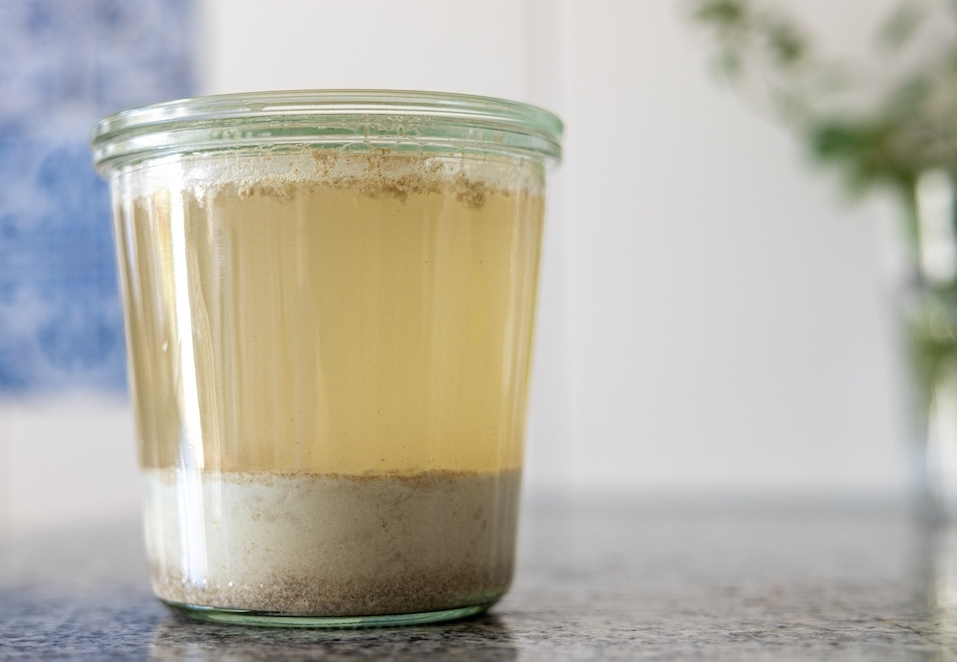
\includegraphics[width=0.5\textwidth]{sourdough-starter-liquid.jpg}
  \caption[Liquid starter]{A liquid sourdough starter features a high level of
      water. The high water amount boosts lactic acid producing bacteria.
      After a while the liquid and flour start to separate. Bubbles on the
      side of the flour indicate that the starter is ready to be used.}%
  \label{fig:liquid-sourdough-starter}
\end{figure}


\begin{flowchart}[!htb]
\centering
  \begin{tikzpicture}[node distance = 5cm, auto]
  \node [start] (init) {Take your regular or stiff starter};
  \node [block, right of=init] (feed_new_ratio) {Mix \qty{1}{\gram} existing starter, \qty{5}{\gram} flour and \qty{25}{\gram} water};
  \node [decision, below of=feed_new_ratio, node distance=5cm] (ready_signs) {Sour yogurty smell and bubbles visible on flour?};
  \node [block, right of=ready_signs, node distance=4cm] (feed_again) {Feed again using 1:5:25 ratio};
  \node [block, left of=ready_signs, node distance=5cm] (last_feed) {Feed one last time};
  \node [success, below of=last_feed, node distance=4cm] (bread_dough) {Make bread dough};
  \path [line] (init) -- (feed_new_ratio);
  \path [line] (feed_new_ratio) -- node{Wait \qty{24}{\hour}} (ready_signs);
  \path [line] (feed_again) -- node[anchor=east]  {} ++(2.2,0) |- (feed_new_ratio);
  \path [line] (ready_signs) -- node{no} (feed_again);
  \path [line] (ready_signs) -- node[above=2pt]{~yes} (last_feed);
  \path [line] (last_feed) -- node{after \qtyrange{6}{12}{\hour}} (bread_dough);
  \draw [thick, ->] ($ (feed_again.north) +(0.7cm, 1cm)$) arc (-45:220:1cm);
  \node [anchor=north, text width=5em] at ($(feed_again.north west)+(1.8cm, 2.3cm)$) {Repeat 3~times};
  
\end{tikzpicture}

  \caption[Converting to a liquid starter]{The process to convert your regular
      or stiff starter into a liquid starter. The whole process takes around 
      3~days. The longer you maintain your starter at the suggested hydration
      level, the more adapted your microorganisms become. It is recommended to
      keep a backup of your original starter as the liquid environment will
      select anaerobic microorganisms. This boosts bacteria that create lactic
      acid rather than acetic acid. The resulting acidity will be perceived as
      milder. When beginning with a liquid starter your stiff starter will
      feature mild dairy notes. When beginning this process with a regular
      starter your created stiff starter will feature both dairy
      and vinegary notes.}%
  \label{flc:liquid-starter-conversion}
\end{flowchart}

The liquid starter is made at a hydration of around \qty{500}{\percent}. This means
the starter has much more water than flour. The additional layer of water on
top of the flour changes the microbiome of your starter.

By introducing this layer of water, less oxygen is available throughout the
course of fermentation. This means that your starter will no longer be
producing acetic acid. The heterofermentative lactic acid bacteria will thrive
in this environment. This is a neat little trick to change your starter's
flavor profile from vinegary to lactic. Your starter is going to develop
dairy creamy notes. Interestingly, when changing the hydration again, your starter
is going to maintain the liquid starter flavor profile, but then benefit again
from enhanced yeast activity. The liquid starter conversion is nonreversible.
By changing to a liquid starter you will permanently select a subset of
microbes that work better in the more liquid environment. So even after going back to a regular
or stiff starter the subset of microbes created by the liquid conversion
will remain. For this reason, it is recommended to keep a backup of the starter
before the liquid starter conversion.

To begin with the
conversion, simply take around \qty{1}{\gram} of your starter, mix with \qty{5}{\gram} flour and
\qty{25}{\gram} water. Stir everything together properly. After a few minutes the flour is
going to start settling in at the bottom of your jar. Repeat this process over
a few days. Shake the starter gently to see if you can see tiny \ch{CO2} bubbles
moving in the liquid. This is a good sign that your starter is ready. Use your
nose to smell the starter. It should have a creamy dairy flavor note.

As you have more bacterial activity, this starter works best with a very strong
flour that can withstand a long fermentation period. Using this starter with a
weak wheat flour will not work. If you do not care about baking a freestanding loaf,
then you can easily use this starter together with a loaf pan.
This starter also works great when making a hearty pancake dough. To use it
I~shake the starter container until I~see all ingredients are homogenized.  Then
I~use around \qty{5}{\percent} of it in terms of baker's math. So for \qty{1000}{\gram} of flour
that's around \qty{50}{\gram} of liquid starter. As it is very liquid you have to
include the \qty{50}{\gram} in your liquid calculation. I~typically treat the starter
directly as liquid in the recipes. So if the recipe calls for \qty{600}{\gram} of water
and I~use \qty{50}{\gram} of starter, then I~would proceed and only use \qty{550}{\gram} of
water.

This type of starter is also an excellent mold combatant. As you are removing
oxygen from the equation, aerobic mold cannot properly grow. If your starter
has a mold problem then the liquid conversion could be the remedy. Take a
piece of your starter where you suspect mold growth. Apply the conversion
as mentioned before. The mold will likely sporulate as it runs out of food.
With each new feeding you are reducing the mold spores. The spores can no
longer reactivate as they cannot do so in the anaerobic conditions.

The liquid on top of your starter is an excellent resource that you could use
to make sauces. If you feel you would like to add a little bit of acidity,
drain the liquid part on your starter and use it. I~have used it numerous
times to make lacto-fermented hot sauces.

\section{Stiff starter}%
\label{section:stiff-starter}

\begin{figure}[!htb]
  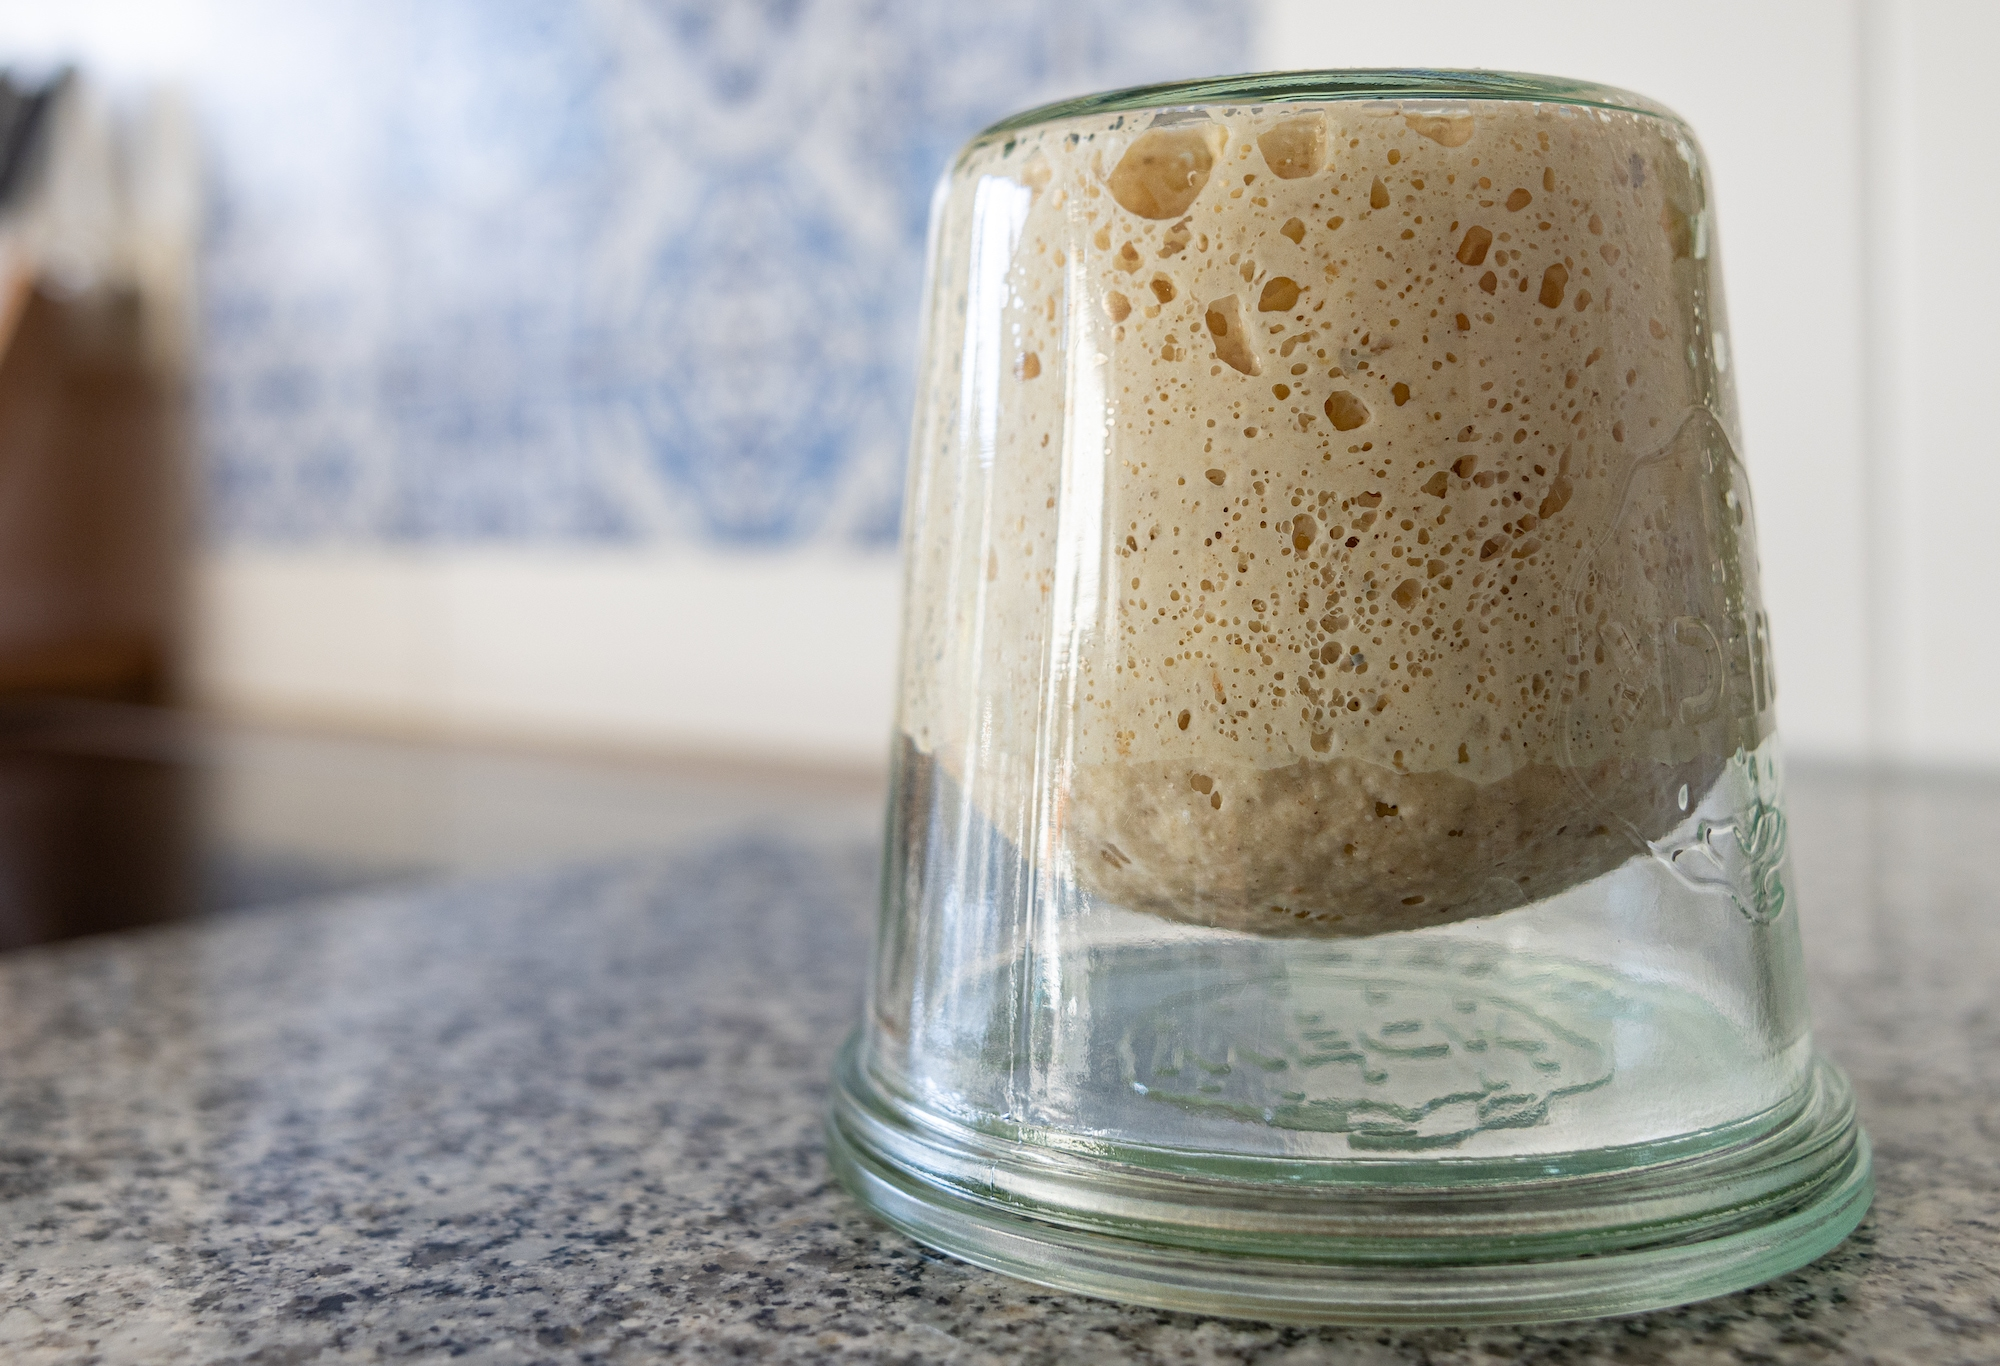
\includegraphics[width=\textwidth]{sourdough-starter-stiff.jpg}
  \caption[Stiff starter upside-down]{A stiff sourdough starter that I~used to
      make a Stollen dough for Christmas. Note the bubbles on the edge of the
      container. The dough does not fall out of the jar. The moment
      the gluten structure breaks down due to fermentation the starter
      will ultimately fall in the jar.}%
  \label{flc:stiff-sourdough-starter}
\end{figure}

The stiff starter is the driest of all the starters. It has a hydration of
around \qtyrange{50}{60}{\percent}. So for \qty{100}{\gram} of flour you are using around
\qtyrange{50}{60}{\gram} of water. If you can't mix flour and water because the
mixture is too dry you need to increase the water quantity. This is often
the case when using whole-wheat/rye flour to make your starter. The
more bran your flour contains, the more water your flour can absorb. The stiff
starter should have a comparable consistency to pasta or pizza dough. When
mixing the starter there should be no chunks of flour left. Test placing
the starter on your kitchen counter. When lifting it should slightly stick
to your counter's surface. This test indicates that you hydrated the flour sufficiently.
When the mixture is too dry, the fermentation speed is greatly reduced and
the starter will seem inactive. The starter should be much drier
than a regular starter, but also not too dry. Refer to figure~\ref{fig:stiff-starter-dry-check}
for a visual example of the starter's required hydration level.

\begin{figure}[!htb]
  \includegraphics[width=\textwidth]{stiff-starter-dry-check.jpg}
  \caption[Too dry and perfectly hydrated stiff starter]{An image showing you a
      stiff starter that is too dry and one that is perfectly hydrated.  The
      starter shouldn't contain chunks of flour and slightly stick to your
      counter top. The starter in the picture is made with whole-wheat flour.}%
  \label{fig:stiff-starter-dry-check}
\end{figure}

\begin{flowchart}[!htb]
\centering
  \begin{tikzpicture}[node distance = 4cm, auto]
  \node [start] (init) {Take your regular or liquid starter};
  \node [block, right of=init, node distance = 4cm] (feed_new_ratio) {Mix \qty{10}{\gram} existing starter, \qty{50}{\gram} flour and \qty{25}{\gram} water};
  \node [decision, right of=feed_new_ratio, node distance=5cm] (too_dry) {Starter very dry, hard to mix?};
  \node [block, right of=too_dry, node distance=4cm] (add_water) {Add more water};
  \node [block, below of=too_dry] (next_day) {Wait\\ \qty{24}{\hour}};
  \node [block] at (feed_new_ratio |- next_day) (feed_again) {Feed again using 1:5:2.5 ratio};
  \node [decision, below of=next_day, node distance=3.5cm] (ready_signs) {Size increase and sour smell?};
  \node [block] at (ready_signs -| add_water) (last_feed) {Feed one last time};
  \node [success, below of=last_feed, node distance=3cm] (bread_dough) {Make bread dough};
  \path [line] (init) -- (feed_new_ratio);
  \path [line] (feed_again) -- (feed_new_ratio);
  \path [line] (next_day) -- (ready_signs);
  \path [line] (ready_signs) -- node{no} (feed_again |- last_feed) |- (feed_again.south);
  \path [line] (ready_signs) -- node{yes} (last_feed);
  \path [line] (last_feed) -- node{after \qtyrange{6}{12}{\hour}} (bread_dough);
  \path [line] (feed_new_ratio) -- (too_dry);
  \path [line] (add_water.north) -- node{} ++(0, 1.3) -| (too_dry.north);
  \path [line] (too_dry) -- node{no} (next_day);
  \path [line] (too_dry) -- node{yes} (add_water);
  \path [line] (ready_signs) -- node{yes} (last_feed);
  \draw [thick, <-] ($ (feed_again.east) +(2.1cm, 0.7cm)$) arc (-45:220:1cm);
  \node [anchor=north, text width=5em] at ($(feed_again.east)+(2cm, 2cm)$) {Repeat 3~times};
\end{tikzpicture}

  \caption[Converting to a stiff starter]{The process to convert your regular
      starter into a stiff starter. The whole process takes around 3 days. The
      longer you maintain your starter at the suggested hydration level, the
      more adapted your microorganisms become. The stiff starter boosts the
      yeast activity of your sourdough starter.  The guide uses a
      \qty{50}{\percent} hydration level for the starter. If the dough is too
      stiff consider increasing this to \qty{60}{\percent}.}%
  \label{fig:stiff-starter-conversion}
\end{flowchart}

In the stiffer environment the yeast thrives more. This means you will have
more \ch{CO2} production and less acid production. In my tests this is a game
changer especially if you are using weaker gluten flours. The wheat flours in
my home country of Germany tend to be lower in gluten. For wheat to build gluten, warm conditions
are preferred~\cite{gluten+development+temperatures}. When following recipes
from other bakers, I~could never achieve similar results. When following
timings my doughs would
simply collapse and become super sticky. Only when I~started to buy more
expensive wheat flour my results did start to change. As not everyone can afford
these special baking flours and due to their limited availability, I~stumbled upon the
stiff sourdough starter. I~made several tests where I~used the same amount of
starter and flour. I~only changed the hydration between all the starters.
I~would then proceed and place a balloon on top of each of the jars. The stiff
starter jar was clearly inflated the most. The regular starter
followed in second place. The liquid starter finished in third place with far less \ch{CO2}
production.

\begin{figure}[!htb]
  \includegraphics[width=\textwidth]{stollen}
  \caption[Christmas \emph{Stollen}]{A German Christmas \emph{Stollen} made
      with a stiff starter instead of yeast.}%
  \label{fig:stollen}
\end{figure}

I~then proceeded and bought a cheap low-gluten cake flour in my nearby supermarket.
This flour before had caused me massive headaches in the past. I~made a sourdough bread
exactly how I~would normally do---I~had to reduce the hydration a bit as a low
gluten flour does not soak up as much water. Then I~replaced the starter with
the stiff starter. The dough felt amazing and was suddenly able to withstand a
much longer fermentation period. The bread had great oven spring and tasted
very mild. I~am still yet to find a proper scientific explanation why the yeast part of
the dough is more active. Maybe it is not. It could also be that the bacteria
is inhibited by the lack of water.

When making the stiff sourdough starter, start by using around \qty{50}{\percent}
water. If you are using a whole-wheat flour, or a strong flour consider going
up to \qty{60}{\percent}. All the ingredients should mix together very well. There
should be no crumbly flour left. This is a common mistake I~have seen when
people tried to make the stiff starter. Yes it should be dry, but not to a
point where it is a brick of cement. If you have ever made a pasta dough, this
dough should feel exactly the same.

To evaluate whether your stiff starter is ready, look for a dome. Also look for
pockets of air on the sides of your container. Use your nose to smell the
starter. It should have a mild smell. It also tends to smell much more
alcoholic than the other starters.

When using a stiff starter, use around \qtyrange{1}{20}{\percent} starter in terms of
baker's math for your
dough. This depends on the ripeness of your starter.
In summer I~typically use around
\qtyrange{1}{10}{\percent} and in winter around \qty{20}{\percent}. This way you can
also control the fermentation speed. If it is very hot where you live, consider
lowering the starter amount to \qtyrange{1}{5}{\percent}. If it is very cold in your
area consider increasing the starter amount up to \qty{30}{\percent}.
Mixing the stiff starter can be a little bit annoying as it hardly homogenizes with
the rest of the dough. In this case, you can try to dissolve the starter in the
water you are about to use for your dough. This will make mixing a lot easier.


\section{Lievito madre or pasta madre}

The \emph{lievito madre}, also known as \emph{pasta madre}, belongs to the
same category as the stiff sourdough starter. After conducting hours of
research, I~could not find a difference between \emph{pasta madre} and
\emph{lievito madre}. Both terms seem to be used interchangeably in
literature.

In many recipes this starter is made directly
from dried or fresh fruits. You can also make a starter from leaves from your
garden. As described before, the wild yeast and bacteria consume the glucose
from the plants' leaves. All the options work. When making a starter directly
from dried fruits, you sometimes lack the bacterial part of the fermentation.
The acidity is very important in order to clean your starter from possible
pathogens. If you decide to make your starter from fruits, make sure it also
acidifies properly when making a dough. A tool such as a pH meter can be of
optimal help. Generally, the lower the pH, the higher the acidity. The acidity
should be below 4.2 to know that your starter produces sufficient acidity.

Some bakers cleanse the \emph{lievito madre} in a bath of water. This is supposed to
remove excess acidity. In my own experiments I~have not been able to confirm
this methodology. The acidity remains the same. The only reason this could
make sense is if you also tried to boost anaerobic microorganisms. However, then the
starter would need to remain in this environment for quite some time and not just
a few hours.

\section{Conclusion}%
\label{sec:starter-type-conclusion}
Baking with sourdough is simple. It's just flour and water. When seeing a recipe
from an experienced baker you wonder, Wait, that's it? There is nothing more
to it? I~feel that this might be the reason why some bakers have such complicated
feeding procedures. They resort to several feedings per day at a certain given ratio.
This makes the baker feel a little more elitist. Of course over time as
more and more people follow this procedure, it became a self fulfilling prophecy.
The more experienced you become, the higher the chances are that a bogus starter
feeding guide will reward you with beautiful results. The reason however is
not in the starter routine. The reason is that you understand the fermentation better
and become better at reading the signs of your dough.

If I~had to choose one starter type I~would go for the stiff starter. In many cases
it will provide you with consistently great results with little effort.
In my experience you can make any yeast-based dough and just replace
the yeast directly with the stiff sourdough starter. You will be able
to achieve even better results with the stiff starter.

Lastly, no matter which starter type you choose, you can control how sour
you want your dough to be. The longer you push the fermentation, the more
acidity is going to be piled up. The only difference is that for a given
volume increase, the stiff starter will produce the least acidity. So for a
volume increase of \qty{100}{\percent}, the liquid starter has produced the most acidity,
followed by the regular starter and then the stiff starter. If you wait long
enough, the stiff starter will have produced the same amount of acidity as the
other starters. But before doing so it will have also produced a lot more \ch{CO2}. If
you like the sour flavor, you have to push your fermentation longer. This also
means you either need to bake in a loaf pan or have a very strong gluten flour
that is able to withstand long fermentation times.


\chapter{Flour types}%
\label{ch:flour-types}
\begin{quoting}
In this chapter we will have a closer look at different flour types
and their respective categorization. We will also look at common
ways to distinguish different flours of the same type, this way you can more
confidently purchase the flour you need.
\end{quoting}

The most basic flour type is a whole grain flour, in this case the whole seed has
been grounded to smaller pieces. Sometimes, depending on what you want to bake,
the hearty taste of the bran might not be desired. In this case you can use
whiter flours. Together with sieves, mills remove larger parts of the seed's
hull.  The seed already contains a pre-built germ from the plant waiting to be
activated. The whitest flour you can get is mostly just the starch part of the seed.
Depending on which layers are still present, different names are used to describe the
type of flour.

\begin{table}[!htb]
    \centering
        \begin{tabular}{@{}llrrr@{}}
\toprule
\textbf{USA}  & \textbf{UK}  & {\textbf{Germany}} & {\textbf{France}} & {\textbf{Italy}} \\ \midrule
Cake         & Soft flour  &  T405            &  T45        & 00 \\ 
All purpose  & Plain flour &  T550            &  T55        & 0 \\ 
Bread flour  & Bread flour &  T405 or T550    &  T45 or T55 & 00 or 0 \\ 
             &             &  T812            &  T80        & 1 \\ 
             &             &  T1050           &  T110       & 2 \\ 
Whole        & Whole       &  Vollkorn        &  T150       & Integrale \\ \bottomrule
\end{tabular}

        \caption[Labelling of wheat flour]{A comparison of how different types
            of wheat flour are labelled in different countries.}%
        \label{tab:flour-types-comparison}
\end{table}

In Germany, the ash content is used to describe the flours. The lab will burn
\qty{100}{\gram} of flour in the oven. Then afterwards the remaining ash is extracted
and measured. Depending on the quantity the flour is categorized. If the flour
is of type 405, then \qty{405}{\mg} of ash have remained after burning the
flour. The more hull parts the flour has, the more minerals remain, therefore the
higher the number, the closer the flour is to whole flour. The numbers are
slightly different between each grain type. Generally though, the higher the
value, the heartier the taste is going to be.

\begin{figure}[htb!]
  \includegraphics[width=\textwidth]{wheat-kernel-overview}
  \caption[Content of a wheat kernel]{An overview of a wheat kernel together
      with its content~\cite{wheat+kernel}.}%
  \label{fig:wheat-kernel-overview}
\end{figure}

If you compare different grain types, there are grains with high gluten, low gluten
and no gluten. Gluten is what enables bread to have its fluffy consistency.
Without gluten the baked goods wouldn't have the same properties. Managing
gluten makes the whole bread-making process more complex as more steps are involved.

A dough without gluten doesn't have to be kneaded as the role of kneading is
to create
the gluten bonds. The more you knead, the stronger they become. With low-gluten
and no-gluten flours, you only have to mix the ingredients together, making
sure you properly homogenize everything.

During fermentation
the gluten degrades as the microorganisms metabolize it. When too much gluten
has been converted your dough will no longer have the wheat-like structure previously
described. For no/low gluten flour your main focus is managing acidity, you do not
want the final bread to be too sour. Conversely you do not have to worry about
the gluten degradation, removing a huge headache from the equation.

\begin{table}[!htb]
    \centering
        \begin{tabular}{@{}lcccc@{}}
\toprule
\textbf{Grain type}        & \textbf{Homogenize} & \textbf{Knead} & \textbf{Stretch \& Fold} & \textbf{Shape} \\ \midrule
Spelt, Wheat (\textgreater{}~70\%) & Yes & Yes & Yes & Yes \\
Rye, Emmer, Einkorn, Rice, Corn    & Yes & No  & No  & No  \\ \bottomrule
\end{tabular}

        \caption[Different types of grain]{An overview of different grain
          types and the steps involved in the respective bread making process.}
\end{table}

Because gluten has a special role, the rest of this chapter is dedicated to having a
closer look at different gluten flours and how to distinguish them. Like wheat
spelt contains significant amounts of gluten, so the same characteristics hold
true.

Several recipes call for wheat bread flour, but bread flour can refer to different types
of flour. It could be a T405 or a T550 in Germany---this is very often
classified incorrectly---the terms \emph{strong} or \emph{bread} flour in this case
refer to the properties of the flour. A bread flour is considered to have a
higher amount of protein and thus gluten. This flour is excellent when you
want to make a sourdough bread as your dough allows for a longer leavening
period. As described earlier, the gluten is consumed by your microorganisms.
The more gluten you have, the longer your dough keeps its integrity. If you wanted
to make a cake, you might want to use a flour with less gluten. The gluten binding
properties might not be desirable since the final cake could have a chewy texture.

In conclusion, not every T405, T45 or T00 flour is the same. Depending on the properties
of the plant they come from, the flours will have different properties. For that reason
some countries like Germany have introduced additional scales to evaluate the quality of the
wheat. The category \emph{A} refers to good quality wheat that can be blended
with poorer qualities to improve the flour. The category \emph{B} refers to
average wheat that can be used to create different baked goods. Category \emph{C}
is used for wheat that has poor baking qualities. This could happen, for instance,
if the wheat already started to sprout and thus lost some of its desirable
baking properties. This type of wheat is typically used in animal feed or
as fermentable biomass for generators. Category \emph{E} refers to \emph{Elite} wheat. It's
the highest quality of wheat. This kind of wheat can only be harvested when the
wheat has grown under optimal conditions. You can compare this to a winery
that uses only the best grapes to make a reserve wine. Unfortunately, this is
usually not printed
on the packaging of the flour that you buy. You can look out for the protein
value as a possible indicator. However, large mills blend flours together to
maintain quality throughout the years. Blended flour is also not listed on
the packaging. It might be that bakeries extract gluten from some flour and
then mix it in order to create better baking flours.

In Italy the so-called
\emph{W-value} has been introduced to better show how the flour will behave.
A dough is made, and then the resistance of this dough to kneading is measured.
The more gluten a flour has, the more elastic the dough is, and the more it will
resist kneading. A higher W flour will have a higher gluten content and allow for a longer
fermentation period. But at the same time, it is also harder for the microbes to
inflate the dough as there is more balloon material. To make an excellent fermented
product out of a high W flour you will need to have a long fermentation period.
The long fermentation period also means that your microbes will enrich
your dough with more flavor.

\begin{table}[!htb]
    \centering
        \begin{tabular}{@{}rcll@{}}
\toprule
\textbf{W-Value} & \textbf{Hydration (\%)} & \textbf{Uses} & \textbf{Fermentation time} \\ \midrule
0--150          & 50     & Cookies             & Very short    \\ 
150--250        & 50--60 & Cakes, Bread, Pizza & Short--Medium \\ 
250--350        & 60--70 & Bread, Pizza        & Long          \\ 
350+            & 70--90 & Bread, Pizza        & Very long     \\ \bottomrule
\end{tabular}

        \caption[Fermentation time versus W-value]{An overview of different
            levels of W-values and the respective hydrations and fermentation
            times.}%
        \label{tab:w-value}
\end{table}

Generally, when aiming to
bake free standing sourdough bread, aim for a higher protein content. If the
gluten value is relatively low, your bread will collapse faster. Baking bread
is still possible, but it might be easier to use other techniques such as a
loaf pan, to consider skillet bread or flatbread.

An additional, rarely considered characteristic of good flour is the level of damage to the
starch molecules. This is a common problem when you are trying to mill your own wheat flours at
home. The chances are that your home mill is not able to achieve the same results
a larger mill can. The damaging of the starches is essential to improve the
properties of the dough. You will have better gelatinization and water
absorption with properly damaged starch~\cite{starch+damage+flour}. As more
starch is damaged, the surface area increases. This improves how water interacts with the flour.
This also provides a larger surface that your microbes can use to attack the molecules
and start the fermentation process.

I~am still
yet to find a good way of milling my own wheat flour at home. Even after trying to
mill the flour 10~times with short breaks, I~was not able to achieve the same
properties as with commercially milled flour. The doughs I~would make felt
good, maybe a bit coarse. However, during baking the doughs would start to
de-gas quickly and turn into very flat breads. I~have had great success though when
utilizing home-milled flour together with a loaf pan or as a pan bread. If you
have found great ways to work with home-milled flour, please reach out. The potential
of using home-milled flours is huge. It would enable even distant communities
to grow their own wheat and be able to produce amazing freshly baked bread.


\chapter{Bread types}%
\label{ch:bread-types}
\begin{quoting}
In this chapter you will learn about different bread types and their
advantages and disadvantages.  You can also find very simple recipes for
flatbread and pan loaf.  The former is probably the most accessible, least
effort type of bread you can make, while the latter is a little more involved.
Free standing bread has its own chapter, due to its increased complexity.
\end{quoting}

\section{Introduction}%
\label{sec:intro}

In this section we classify bread by its baking techniques. The appearance and
taste will of course be different, but you can get excellent bread with each
of them. Some breads will require investment and technique, as depicted in
Table~\ref{tab:bread-types-comparison}.  Flatbread is probably the most
accessible, least effort type of bread you can make. If you are a busy person
and/or don’t have an oven, this might be exactly the type of bread you should
consider. 
\begin{table}[!htb]
    \centering
        \begin{tabular}{@{}llll@{}}
\toprule
                    &             \multicolumn{3}{c}{\textbf{Type of bread}}\\
                                  \cmidrule(lll){2-4}
                    & \textbf{Flat}       & \textbf{Loaf pan} &  \textbf{Free standing} \\ \midrule
Cooking method      & Pan, fire, barbecue & Oven              & Oven                    \\ 
Working time        & 3~min.              & 5~min.            & 60~min.                 \\ 
Flour types         & All                 & All               & Gluten flours           \\ 
Difficulty          & Very easy           & Easy              & Difficult               \\ 
Cost                & Low                 & Medium            & High                    \\ \bottomrule
\end{tabular}

        \caption[Different bread types]{An overview of different bread types
            and their respective complexity.}%
        \label{tab:bread-types-comparison}
\end{table}

\section{Flatbread}%
\label{sec:flatbread}

Flatbread is probably the simplest sourdough bread to make.
To make a flatbread no oven is required; all you need is a stove.

\begin{figure}[!htb]
  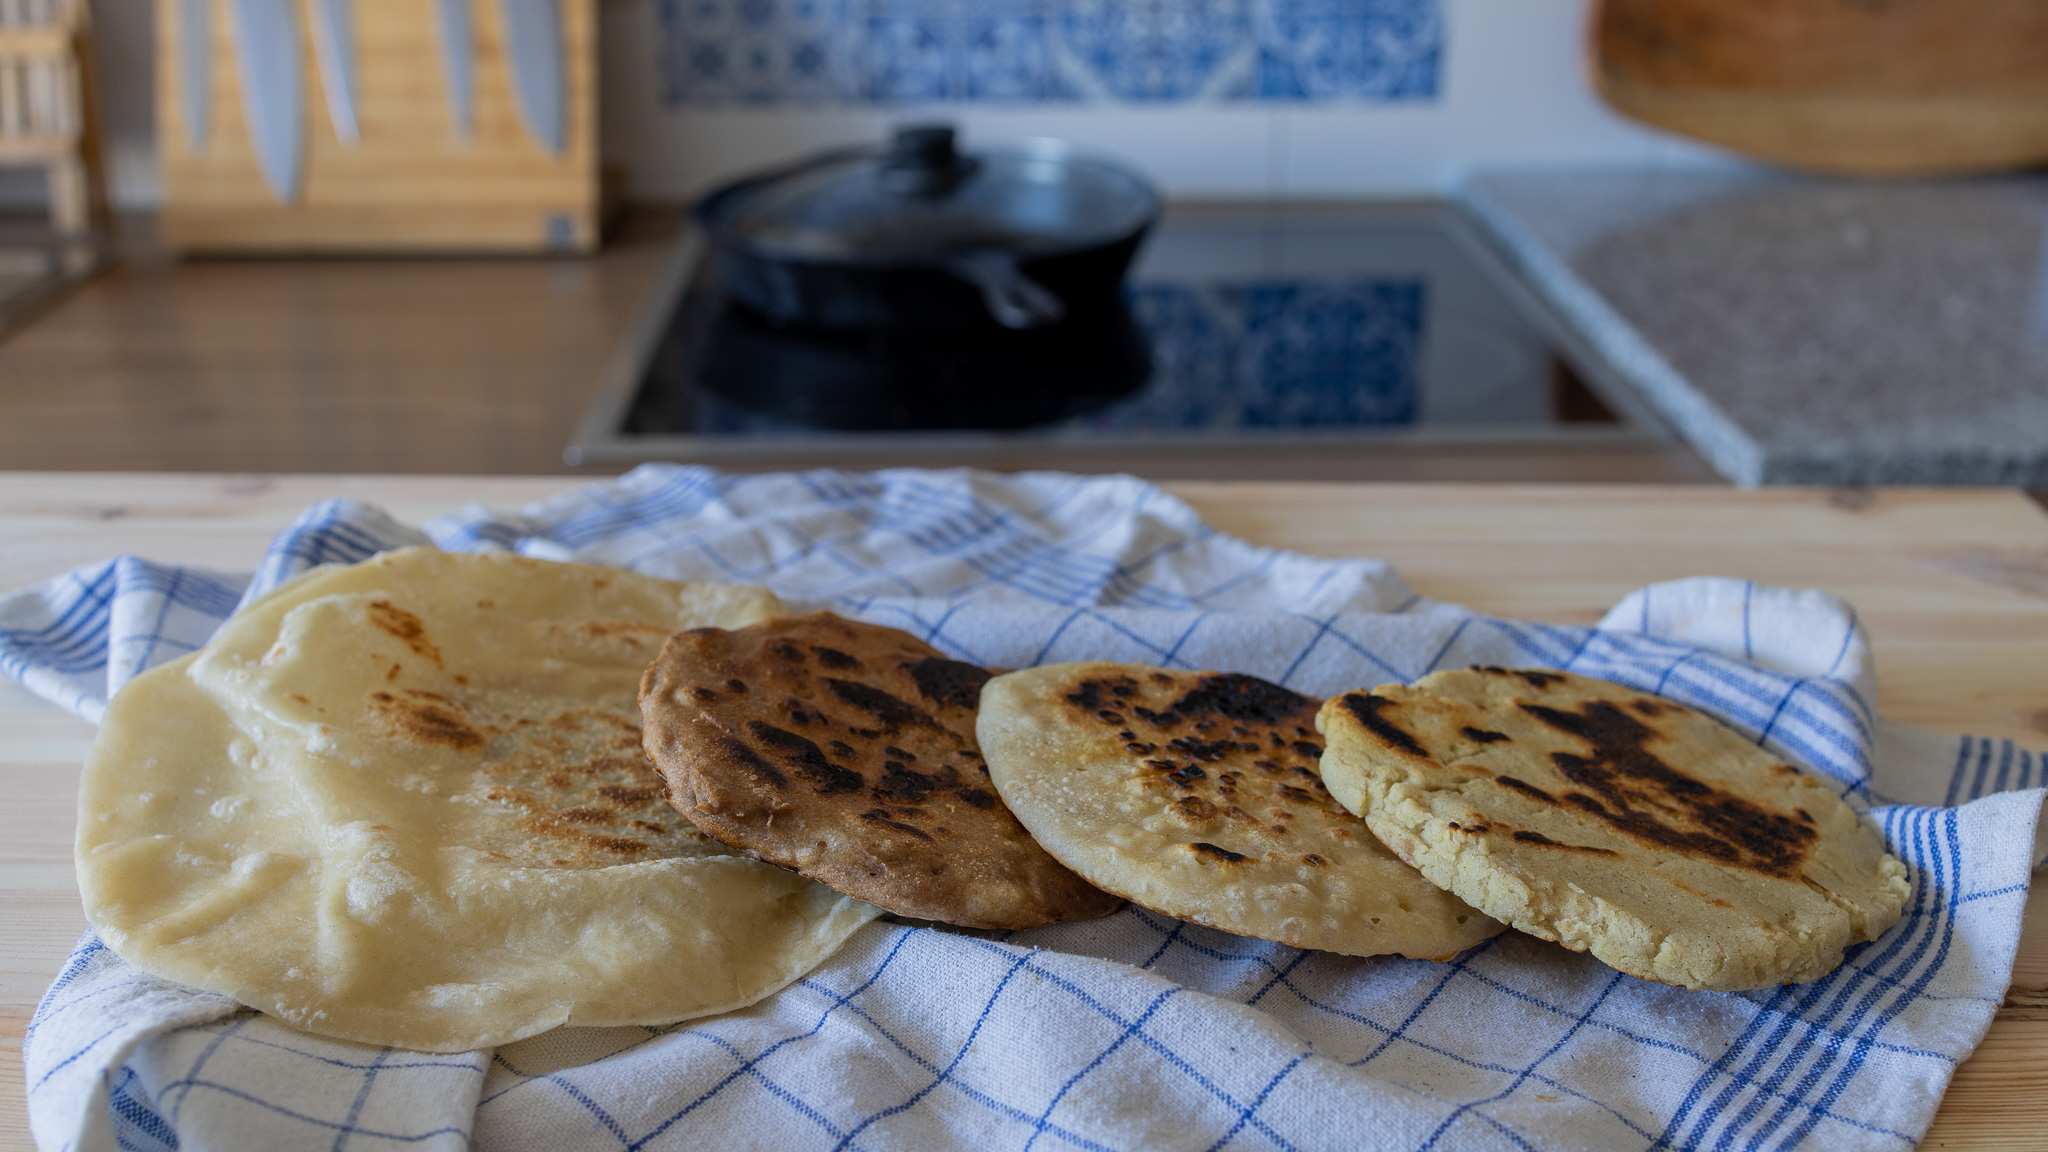
\includegraphics[width=\textwidth]{flat-breads-selection}
  \caption[Flatbread selection with different flours]{An assorted selection of
      different flatbreads made with sourdough. From left to right:
      Wheat~tortilla, rye, spelt and corn.}%
\end{figure}

This type of bread is super simple to make as you can skip
a lot of the technique that is normally required to make wheat doughs.
The flatbread can be made with all kinds of flours. You can even use
flour without gluten, such as corn or rice flour, to make the
dough. To make the flatbread a little more fluffy, you
can use a little bit of wheat flour. The developing gluten
will trap the gases. During baking, these gases will
inflate the dough.

Another trick to improve the texture of the flatbread is to
make a very wet dough. A lot of the water will evaporate
during the baking process and thus make the bread fluffier.
If your water content is very high, it will produce a
pancake-like consistency, as you can see in
Table~\ref{tab:flat-bread-ingredients}

\begin{table}[!htb]
    \centering
        %TODO: Alignement is not great
\begin{tabular}{@{}lll@{}}
\toprule
                  & \textbf{Flat breads}           & \textbf{Pancakes}          \\ \midrule
Flour             & \qty{100}{g}                   & \qty{100}{g}                       \\ 
Water             & up to \qty{100}{g} (\qty{100}{\percent})     & \qty{300}{g} (\qty{300}{\percent})               \\ 
Sourdough starter & 5--\qty{20}{g} (5--\qty{20}{\percent})       & 5--\qty{20}{g} (5--\qty{20}{\percent})           \\ 
Salt              & \qty{2}{g} (\qty{2}{\percent})               & \qty{2}{g} (\qty{2}{\percent})                   \\ 
        Bake when?        & Dough increased \qty{50}{\percent} in size & Bubbles visible on surface \\ \bottomrule
\end{tabular}

        \caption[Flatbread recipe]{Flatbread or pancake recipe for 1 person.
            Multiply the ingredients to increase portion size.  Refer to the
            Section~\ref{section:bakers-math}
            ``\nameref{section:bakers-math}'' to learn how to understand and
            use the percentages properly.}%
            \label{tab:flat-bread-ingredients}
\end{table}

For a full recipe including the process of making such a flatbread,   refer to
Subsection~\ref{subsec:flat-bread-recipe}

\subsection{Flatbread framework}%
\label{subsec:flat-bread-framework}

As explained above, if you are just getting started, making a flatbread is the
easiest way to start making great bread at home. With just a
few steps, you can stop buying bread forever. This works with
any flour, including gluten-free options.

\begin{flowchart}[!htb]
\centering
  \input{figures/fig-process-flat-bread.tex}
  \caption[The process to make a sourdough flatbread]{The process of making a flatbread is very
      simple, requiring very little effort. This type of bread is especially
      handy for busy bakers.}%
  \label{fig:flat-bread-process}
\end{flowchart}

This is my go-to recipe that I~use to make bread whenever
I~have little time or when I~am abroad. You can choose
between two options:
%
\begin{enumerate}
    \item A flatbread similar to a roti or naan bread
    \item Sourdough pancakes.
\end{enumerate}

To get started prepare your sourdough starter. If it has not been used for a very
long time, consider giving it another feed. To do so, simply take \qty{1}{\gram} of your
existing sourdough starter and feed it with \qty{5}{\gram} of flour and \qty{5}{\gram} of water.
If you do this in the morning, your sourdough starter will be ready in the evening. The
warmer it is, the sooner it will be ready,  consider
using warm water if it is very cold where you live.

\begin{figure}[htb!]
\centering
  \includegraphics[width=1.0\textwidth]{flat-bread-wheat}
  \caption[Wheat flatbread]{A flatbread made with purely wheat flour. The
      dough is drier at around \qty{60}{\percent} hydration. The drier dough
      is a little harder to mix. As wheat contains more gluten, the dough
      puffs up during the baking process.}
\end{figure}

This way you should have around \qty{11}{\gram} of sourdough ready in the evening. You will have
the perfect quantity to make a dough for one person. In case you want to make more
bread, simply multiply the quantities shown in
Table~\ref{tab:flat-bread-ingredients}.

Then in the evening simply mix the ingredients as shown in the table. Your dough
is going to be ready in the morning. It's typically ready after 6--12~hours. If
you use more sourdough starter it will be ready faster, conversely it will take
longer if you use less. Try to aim for a fermentation time of 8--12~hours as
by using your dough too soon, the flavor might not be as good. By using your
dough later it might become a little more sour. The best option is to
experiment and see what you personally like the most.

After mixing the ingredients together cover the container, this prevents the
dough from drying out and makes
sure no fruit flies get access. A transparent container will be helpful
when getting started. You can observe the dough more easily and see when
it is ready.

\begin{figure}[htb]
\centering
  \includegraphics[width=1.0\textwidth]{ethiopian-woman-checking-bread}
  \caption[Ethiopian \emph{injera}]{An Ethiopian woman baking an \emph{injera}
      made using teff flour.  The image has been provided by Charliefleurene
      via Wikipedia.}
\end{figure}

If you used the flatbread option with less water, look at the size increase
of your dough. It should have increased at least \qty{50}{\percent} in size.
Also look out for bubbles on the sides of your container.

When using the pancake recipe, look out for bubbles on the surface of your dough.
In both cases use your nose to check the scent of your dough. Depending
on your sourdough starter's microbiome your dough will have
dairy, fruity, alcoholic notes or vinegary, acetic notes. Relying
on the smell of your dough is the best way to judge whether your
dough is ready or not. Timings are not reliable as they
depend on your starter and the temperature. If your dough
is ready too soon, you can now move it directly to the fridge and bake
it at a later, more convenient time. The low temperature will halt the fermentation
process\footnote{There are some exceptions. In some rare cases your starter
might also work at lower temperatures. You might have cultivated microbes that work best at
low temperatures. Nevertheless, fermentation
is always slower the colder it gets. A fridge really helps to preserve the state
of your dough.}
and your dough will last for several days. The longer you wait, the more sour the
bread is going to be. The fridge is a great option in case you want to
take the dough with you when visiting friends. People are going
to love you for the freshly baked flatbreads or pancakes. If you dare,
you can also taste a little bit of your raw uncooked dough. It is likely
going to taste relatively sour. I~do this frequently to better evaluate the
state of my doughs.

\begin{figure}[!htb]
\centering
  \includegraphics[width=1.0\textwidth]{injera-pancake-texture.jpg}
  \caption[Teff sourdough pancake]{A sourdough pancake made with teff flour.
      The pockets come from evaporated water and \ch{CO2} created by the
      microbes.  The image has been provided by Łukasz Nowak via Wikipedia.}
\end{figure}

If you are feeling lazy or don't have time, you could also use older sourdough starter
to make the dough directly without any prior starter feedings. Your sourdough starter
is going to regrow inside your dough. Remember that the
final bread might be a bit more on the sour side as the balance of yeast to
bacteria could be off. In the Table~\ref{tab:flat-bread-ingredients}
I~recommended using around \qtyrange{5}{20}{\percent}
of sourdough starter based on the flour to make the dough. If you were to follow
this approach, just use around \qty{1}{\percent} and make the dough directly.
The dough is probably going to be ready 24~hours later, depending on the temperature.

If you want to make sweet pancakes, add some sugar and optional eggs to your dough
now. A good quantity of eggs is around one~egg per \qty{100}{\gram} of flour.
Stir your dough a little bit and it will be ready to be used. You'll
have delicious sweet savory pancakes, the perfect combination. By
adding the sugar now, you make sure that the microbes don't have
enough time to fully ferment it. If you had added the sugar
earlier, no sweet flavor would be left  12~hours later.

To bake your dough heat your stove to medium temperature. Add a little bit of
oil to the pan. This helps with heat distribution and ensures even cooking.
With a spatula or a spoon place your dough in the pan. If your dough
was sitting in the fridge, bake it directly. There is no need to wait for your
dough to come to room temperature. If you have a lid,
place it on your pan. The lid helps to cook your dough from the top.
The evaporating water will circulate and heat up the dough's surface. When
making a flatbread, make the dough around \qty{1}{\cm} thick. When using the
pancake option, opt for around \qtyrange{0.1}{0.5}{\cm} depending on what you
like.

\begin{figure}[htb]
\centering
  \includegraphics[width=1.0\textwidth]{einkorn-crumb.jpg}
  \caption[Einkorn crum]{The crumb of a flatbread made with einkorn as flour.
      Einkorn is very low in gluten and thus does not trap as much \ch{CO2} as
      a wheat based dough. To make the dough fluffier use more water or
      consider adding more wheat to the mix of your dough.}
\end{figure}

After 2--4~minutes flip over the pancake or flatbread. Bake it for the same
time from the other side. Depending on what you like, you can wait a little
longer to allow the bread to become a bit charred. The longer you
bake your bread, the more of the acidity is going to evaporate. If your
dough is a bit more on the sour side, you can use this trick to balance
out the acidity. This really depends on which flavor you are looking for.

When making a flatbread I~recommend wrapping the baked flatbreads in a kitchen
towel. This way more of the evaporating humidity stays inside of your bread,
making sure your flatbreads stay nice and fluffy for a longer period after the
bake. A similar strategy is used when making corn tortillas.

You can safely store the baked flatbreads or pancakes in your fridge
for weeks. When storing make sure to store them in an airtight plastic bag so that
they do not dry out. If they dry out, spray them with some water and toast them.
They will be almost as good as when they were freshly baked.

Keep a little bit of your unbaked dough. You can use it to make the next
batch of bread or pancakes for the next day. If you want to bake a few days later, add
a little bit of water and flour and store this mixture in your fridge
for as long as you like\footnote{The starter will stay good for months. If you expect to
leave it longer, consider drying a little bit of your sourdough starter.}.

\subsection{Simple flatbread recipe}%
\label{subsec:flat-bread-recipe}

By following the steps outlined in this section,
you'll be introduced to a versatile bread that's perfect for a myriad of
culinary applications. Whether you're scooping up a savory dip,
wrapping a flavorful filling, or simply enjoying a piece with a drizzle
of olive oil, these flatbreads are sure to impress.

\subsubsection*{Ingredients}
\begin{tabular}{r@{}rl@{}}
\qty{400}{\gram} &~(\qty{100}{\percent}) & Flour (wheat, rye, corn, whatever
                                            you have at hand)\\
\qty{320}{\gram} &  (\qty{80}{\percent}) & Water, preferably at room
                                            temperature\\
\qty{80}{\gram}  &  (\qty{20}{\percent}) & Active sourdough starter\\
\qty{8}{\gram}   &   (\qty{2}{\percent}) & Salt\\
\end{tabular}

\subsubsection*{Instructions}
\begin{description}
\item[Prepare the dough] In a large mixing bowl, combine the flour and water.
    Mix until you have a shaggy dough with no dry spots.

    Add the sourdough starter and salt to the mixture. Incorporate them
    thoroughly until you achieve a smooth and homogenized dough.

\item[Fermentation:] Cover the bowl with a lid or plastic wrap. Allow the dough
    to rest and ferment until it has increased by at least \qty{50}{\percent}
    in size.  Depending on the temperature and activity of your starter, this
    can take anywhere from 4 to 24~hours.

\item[Cooking preparation:] Once the dough has risen, heat a pan over medium
    heat.  Lightly oil the pan, ensuring to wipe away any excess oil with a
    paper towel.

\item[Shaping and cooking:] With a ladle or your hands, scoop out a portion of
    the dough and place it onto the hot pan, spreading it gently like a
    pancake.

    Cover the pan with a lid. This traps the steam and ensures even cooking
    from the top, allowing for easier flipping later.

    After about 5~minutes, or when the bottom of the flatbread has a
    golden-brown crust, carefully flip it using a spatula.

    \emph{Adjusting cook time.} If the flatbread appears too dark, remember to
    reduce the cooking time slightly for the next one.  Conversely, if it's
    too pale, allow it to cook a bit longer before flipping.

    Cook the flipped side for an additional 5~minutes or until it's also
    golden brown.

\item[Storing:] Once cooked, remove the flatbread from the pan and place it on
    a kitchen towel. Wrapping the breads in the towel will help retain their
    softness and prevent them from becoming overly crisp.  Repeat the cooking
    process for the remaining dough.

\item[Serving suggestion:] Enjoy your sourdough flatbreads warm, paired with
    your favorite dips, spreads, or as a side to any meal.

\end{description}


\section{Loaf pan bread}%
\label{sec:loaf-pan-bread}

Loaf pan bread is made using the help of a special loaf pan
or loaf tin. The edges of the pan provide additional support
for the dough to rise. Making a bread using a loaf pan requires
an oven.

\begin{figure}[!htb]
  \includegraphics[width=\textwidth]{loaf-pan-free-standing.jpg}
  \caption[Freestanding bread and pan bread]{A freestanding bread and a wheat
      loaf pan bread. Both of them received a small incision before baking
      which helps to control how they open up.}%
  \label{fig:free-standing-loaf-pan}
\end{figure}

After mixing your dough, you can place it directly into the loaf pan.
This makes the whole process simpler since you can skip steps such
as shaping the dough.

To make a great loaf pan bread with little work:

\begin{enumerate}
    \item Mix the ingredients of your dough (gluten free works too)
    \item Place into the loaf pan
    \item Wait until your dough has roughly doubled in size
    \item Bake in a non pre-heated oven for around 30--50~minutes
\end{enumerate}

Knowing the exact baking time is sometimes a little challenging
as it might be that the outside of your bread is cooked but
the inside is still raw. The best way is to use a thermometer
and measure the core temperature. At around  \qty{92}{\degreeCelsius}
(\qty{197}{\degF}) your dough is done. I~generally bake loaf pan bread at
around  \qty{200}{\degreeCelsius} (\qty{390}{\degF}), which is a little less
than my freestanding bread which I~bake at  \qty{230}{\degreeCelsius}
(\qty{445}{\degF}). That's because it takes a while for the dough
to bake properly inside the loaf pan. The edges don't heat up
as quickly. Then the top part of the dough is properly cooked, while
the inside isn't yet. When baking make sure to use steam
or simply place another equally sized loaf pan on top
of your loaf pan. This way you simulate a Dutch oven. The dough's
evaporating moisture will stay inside.

A good trick to make excellent loaf pan bread is to make a very
sticky dough. You can opt for a hydration of \qtyrange{90}{100}{\percent}, almost
resembling a default sourdough starter. Just like with flatbread,
the high humidity helps to make a more airy, fluffy crumb. The bread will
also be a bit chewier. This type of bread made with rye is my family's favorite
style of bread.  The hearty rye flavor paired with the sticky consistency really
makes an excellent sandwich bread.

To improve the structure you can also consider using around \qty{50}{\percent}
wheat flour in your mix. The gluten network will develop as your
dough ferments and allow for more gas to be trapped in the dough.

A common problem you will face when making a loaf pan bread is
the dough sticking to the pan. Use a generous amount of oil to grease
your pan. A nonstick vegetable oil spray can do wonders.
Don't clean your loaf pans with soap. Just use a kitchen towel
to clean them. With each bake a better patina forms, making your
pan more and more stick resistant.

What's amazing about this type of bread is that it works
with every flour. The overall time to work the dough is probably
less than 5~minutes, making it very easy to integrate
into your daily routine. Furthermore, loaf pans use the space
in your oven very efficiently. Using pans I~can
easily bake 5 loaves at the same time in my home oven.
Normally I~would need multiple baking sessions for
freestanding loaves.

\section{Free standing bread}

A freestanding loaf is baked entirely without supporting
baking vessels in your oven. To make a freestanding loaf more steps
and tools are required.

\begin{figure}[!htb]
\centering
  \includegraphics[width=1.0\textwidth]{free-standing-loaf.jpg}
  \caption[Freestanding sourdough bread]{A freestanding sourdough bread. Note
      the incision known as an \emph{ear} and the oven spring clearly
      distinguish this type of bread from flatbread and loaf pan bread.}
\end{figure}

When using wheat, make sure to mix your dough enough to develop a gluten network.
Allow the dough to reach a certain size increase during the fermentation.
Afterward, divide and pre-shape the dough into the desired visual shape you
would like. Each shape requires a different technique. Sometimes achieving
the right shape can be challenging. Making a baguette, for instance,
requires performing more steps. Mastering this technique takes several attempts.

Once the dough is shaped, it is proofed again for a certain
period of time. Once the dough is ready, a sharp tool such
as a razor blade is used to make an incision into the dough.
This helps control how the dough opens up during the baking process.

All these steps require practice. Each of them has to be
performed perfectly, without mistakes.
But after baking you will be rewarded with a beautiful bread
with great taste and consistency.

There is a dedicated recipe and tutorial for this type of bread in the
\nameref{chapter:wheat-sourdough} chapter.


\chapter{Wheat sourdough}%
\label{chapter:wheat-sourdough-translated}
\input{wheat-sourdough/wheat-sourdough-translated}

\chapter{Non wheat sourdough}%
\label{chapter:non-wheat-sourdough}
\begin{quoting}
In this chapter you will learn how to make a basic sourdough bread
using non-wheat flour, basically all flour except spelt.
The key difference between wheat and non-wheat flour is
the quantity of gluten, the former feature a high amount
of gluten, while the non-wheat flours do not.
\end{quoting}

The whole process (see Flowchart~\ref{flc:non-wheat-sourdough}) is a lot
easier: you mix the ingredients and wait for a certain period until the dough
has reached the level of acidity that you like.  Afterward, you shape the
dough or pour it into a loaf pan. After a short proofing period, the bread can
be baked. Due to the lack of gluten development, the final bread will feature
a denser crumb compared to wheat, as you can see in
Picture~\ref{fig:rye-crumb}.

\begin{flowchart}[!htb]
\centering
  \begin{tikzpicture}[node distance = 3.8cm, auto]
  \node [start] (init) {Mix \\ingredients};
  \node [block, below of=init, node distance = 3cm] (bulk_ferment) {Bulk ferment};
  \node [block, right of=init] (divide) {Divide};
  \node [block] at (divide |- bulk_ferment) (shape) {Shape};
  \node [block, right of=divide] (proof) {Proof};
  \node [success] at (proof |- bulk_ferment) (bake) {Bake};
  \path [line] (init) -- (bulk_ferment);
  \path [line] (bulk_ferment.north east) -- (divide.south west);
  \path [line] (divide) -- (shape);
  \path [line] (shape.north east) -- (proof.south west);
  \path [line] (proof) -- (bake);
\end{tikzpicture}

  \caption[Process for non-wheat sourdough bread]{A visualization of the
      process to make non-wheat sourdough bread.  The process is much simpler
      than making wheat sourdough bread. There is no gluten development. The
      ingredients are simply mixed together.}%
  \label{flc:non-wheat-sourdough}
\end{flowchart}

For non-wheat flours---including rye, emmer, and einkorn---no gluten
development has to be done, meaning there is no kneading, no
over-fermentation, and no issues with making flat bread.  In the case of rye
flour, sugars called pentosans prevent gluten bonds from properly
forming~\cite{rye+pentosans}.

\begin{figure}[!htb]
  \includegraphics[width=\textwidth]{final-bread}
  \caption[Sourdough rye bread]{A sourdough rye bread made using a loaf pan.
      The rye bread is not scored. The crust typically cracks open during
      baking.}%
  \label{fig:non-wheat-final-bread}
\end{figure}


This chapter will focus on making rye bread. The flour could
be replaced with einkorn or emmer based on your preference.

The following recipe will make you 2 loaves:

\begin{tabular}{r@{}rl@{}}
    \qty{1000}{\gram} &~(\qty{100}{\percent}) & Whole rye flour\\
    \qty{800}{\gram}  &  (\qty{80}{\percent}) & Water at room temperature\\
    \qty{200}{\gram}  &  (\qty{20}{\percent}) & Sourdough starter\\
    \qty{20}{\gram}   &   (\qty{2}{\percent}) & Salt\\
\end{tabular}

The sourdough starter can be in an active or inactive state. If it has been
at room temperature for a week with no feedings then it will be okay, same
if it has come right out of the fridge then still it will be no problem.
The dough is very forgiving.

If you follow the suggested quantities from the recipe you are making a
relatively wet rye dough. It's so wet that it can only be made using a loaf
pan. If you want to make a freestanding rye bread, consider reducing the
hydration to around~\qty{60}{\percent}.

\begin{figure}[!htb]
  \includegraphics[width=\textwidth]{ingredients}
  \caption[Non-wheat dough]{For non-wheat dough the ingredients are mixed
      together. There is no need to develop any dough strength. This
      simplifies the whole bread-making process.}%
  \label{fig:non-wheat-ingredients}
\end{figure}

Mix together all the ingredients with your hands, or opt for a spatula to
simplify things. Rye flour itself is very sticky and unpleasant to mix by
hand, the dough will stick a lot to your hands. If you use a stiff starter, it
could be easier to first dissolve it in the dough's water, then add the other
ingredients.

\begin{figure}[!htb]
  \includegraphics[width=\textwidth]{sticky-hands}
  \caption[Sticky rye dough]{Rye flour has a sugar molecule known as pentosan.
      These pentosans prevent the rye flour from building gluten bonds. As a
      result the dough never features an open crumb and is always very sticky
      when hand mixing.}%
  \label{fig:non-wheat-sticky-hands}
\end{figure}

The goal of the mixing process is simply to homogenize the dough, there
is no need to develop any dough strength. Once you see that
your sourdough starter has been properly incorporated, your
dough is ready to begin bulk fermentation.

You can bulk ferment the dough for a few hours up to
weeks. By extending the bulk fermentation time, you increase
the acidity the final loaf is going to feature. After around
48~hours, the acidity will no longer increase. This is because
most of the nutrients have been eaten by your microorganisms.
You could let your dough sit for longer, but it wouldn't alter the
final flavor profile by much.

I~recommend waiting until the dough has roughly increased
by~\qty{50}{\percent} in size. If you are daring, you can taste the dough to
get an idea of the acidity profile, it will likely taste very sour. However, a
lot of the acid will evaporate during the baking process, therefore the final
loaf will not be as sour as the dough you are tasting.

\begin{figure}[!htb]
  \includegraphics[width=\textwidth]{crumb}
  \caption[Rye bread]{The crumb structure of rye bread. By making a wetter
  dough, more water evaporates during the baking and thus the
  crumb tends to be a bit more open. Generally, rye
  bread is never as fluffy as wheat sourdough bread. The crust
  of this bread is a bit pale. The crust color can be controlled
  by baking the bread for a longer period.}%
  \label{fig:rye-crumb}
\end{figure}

Once you are happy with the acidity level, proceed to dividing
and shaping your dough.  If you made a drier dough, use as much
flour as needed to dry the dough a little bit and form a dough ball.
There is no folding the dough. All you do is tuck it together
as much as is needed to apply the shape of your banneton.

Shaping might not be possible if you opt for the wetter dough. Carefully spread
the dough with a spatula in your greased loaf pan, wetting the spatula to make
this process easier. Spread it until the surface looks smooth and shiny.

For proofing, I~recommend waiting around 60~minutes. An extended
proofing period does not make sense unless you want to further
increase the dough's acidity. The dough will not become fluffier
the longer you proof. With the short proofing period, however,
the dough will become a bit more homogeneous. This way the final
bread looks more uniform. The proofing period also allows the
dough to fully extend and fill the edges of the loaf pan. I~also
like to move the dough to the fridge for proofing. The dough stays
good in the fridge for weeks. You can proceed and bake it at a
convenient time for you. 

Once you are happy with the proofing stage, proceed and bake your dough
just like you'd normally do, more details can be found in
Chapter~\ref{chapter:baking}. One challenging aspect
of using a loaf pan is to make sure that the center part of your
dough is properly cooked. For this reason, it is best to use a thermometer
and measure the internal temperature. The bread is ready once the internal
temperature reaches \qty{92}{\degreeCelsius} (\qty{197}{\degF}). I~recommend
removing the bread from the loaf pan once it reaches the desired temperature,
then continue baking the loaf without the pan and steam. This way you achieve
a great crust all around your loaf, and can bake as long as you like until you
have achieved your crust color of choice. The darker, the more crunchy
the crust and the more flavor it offers. If you feel your dough might have
been overly acidic you can extend the baking time, as the longer you bake, the
more acidity will evaporate.

This is one of my favorite breads to bake which I~eat on an
almost daily basis. The effort required to make bread like
this is much lower compared to a wheat-based dough. In some
cases, I~extend the recipe and add additional sourdough discard
to the dough. You can add as much discard as you like. The resulting
bread will have a very complex but delicious flavor profile.


\chapter{Mix-ins}%
\label{ch:mix-ins}
\begin{quoting}
  In this chapter, you will learn about the fascinating world of sourdough
  mix-ins. Discover how these additions can elevate your bread, enhancing
  flavor, adding vibrant colors, and creating delightful textures that make
  each loaf a culinary masterpiece.
\end{quoting}

\begin{figure}[htb!]
  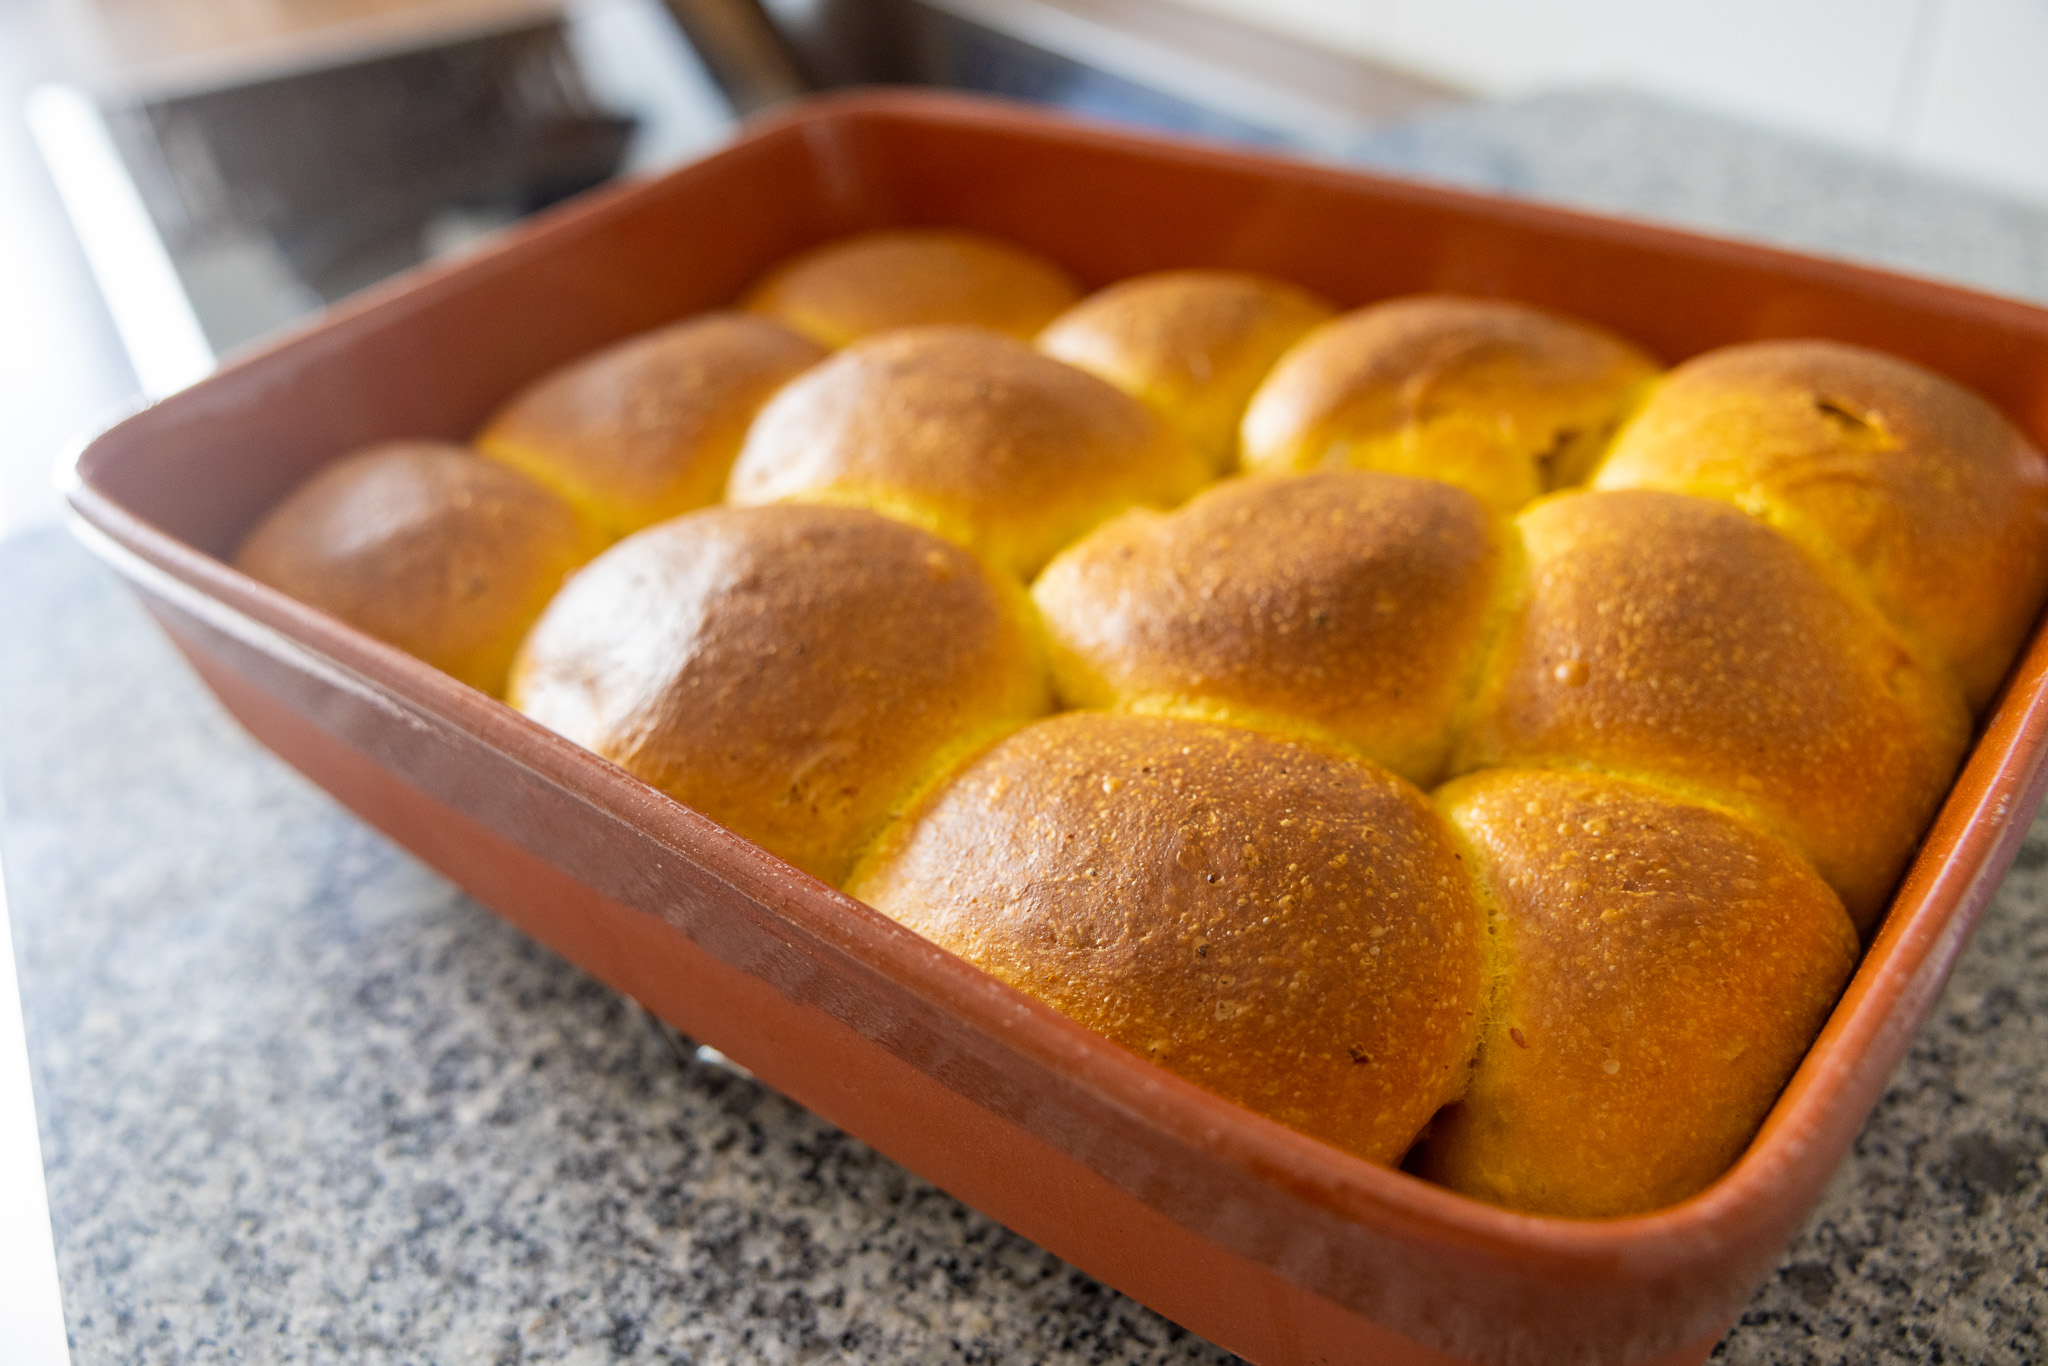
\includegraphics[width=\textwidth]{pumpkin-sourdough}
  \caption[Pumpkin sourdough softbuns]{These soft pull-apart sourdough
    buns have been made with the addition of pumpkin purée. The mashed pumpkin
    adds flavor and hydration to the dough.}%
\end{figure}

A loaf of wheat sourdough has a very pure aesthetic. Good craftsmanship and
precision transform the ingredients into simple, but delicious food. With
mix-ins, the basic recipe can become the starting point for a whole world of
modifications to try and combine. Think of the loaf of bread as a blank canvas
to express yourself.

\section{Categories}

\begin{figure}[htb!]
  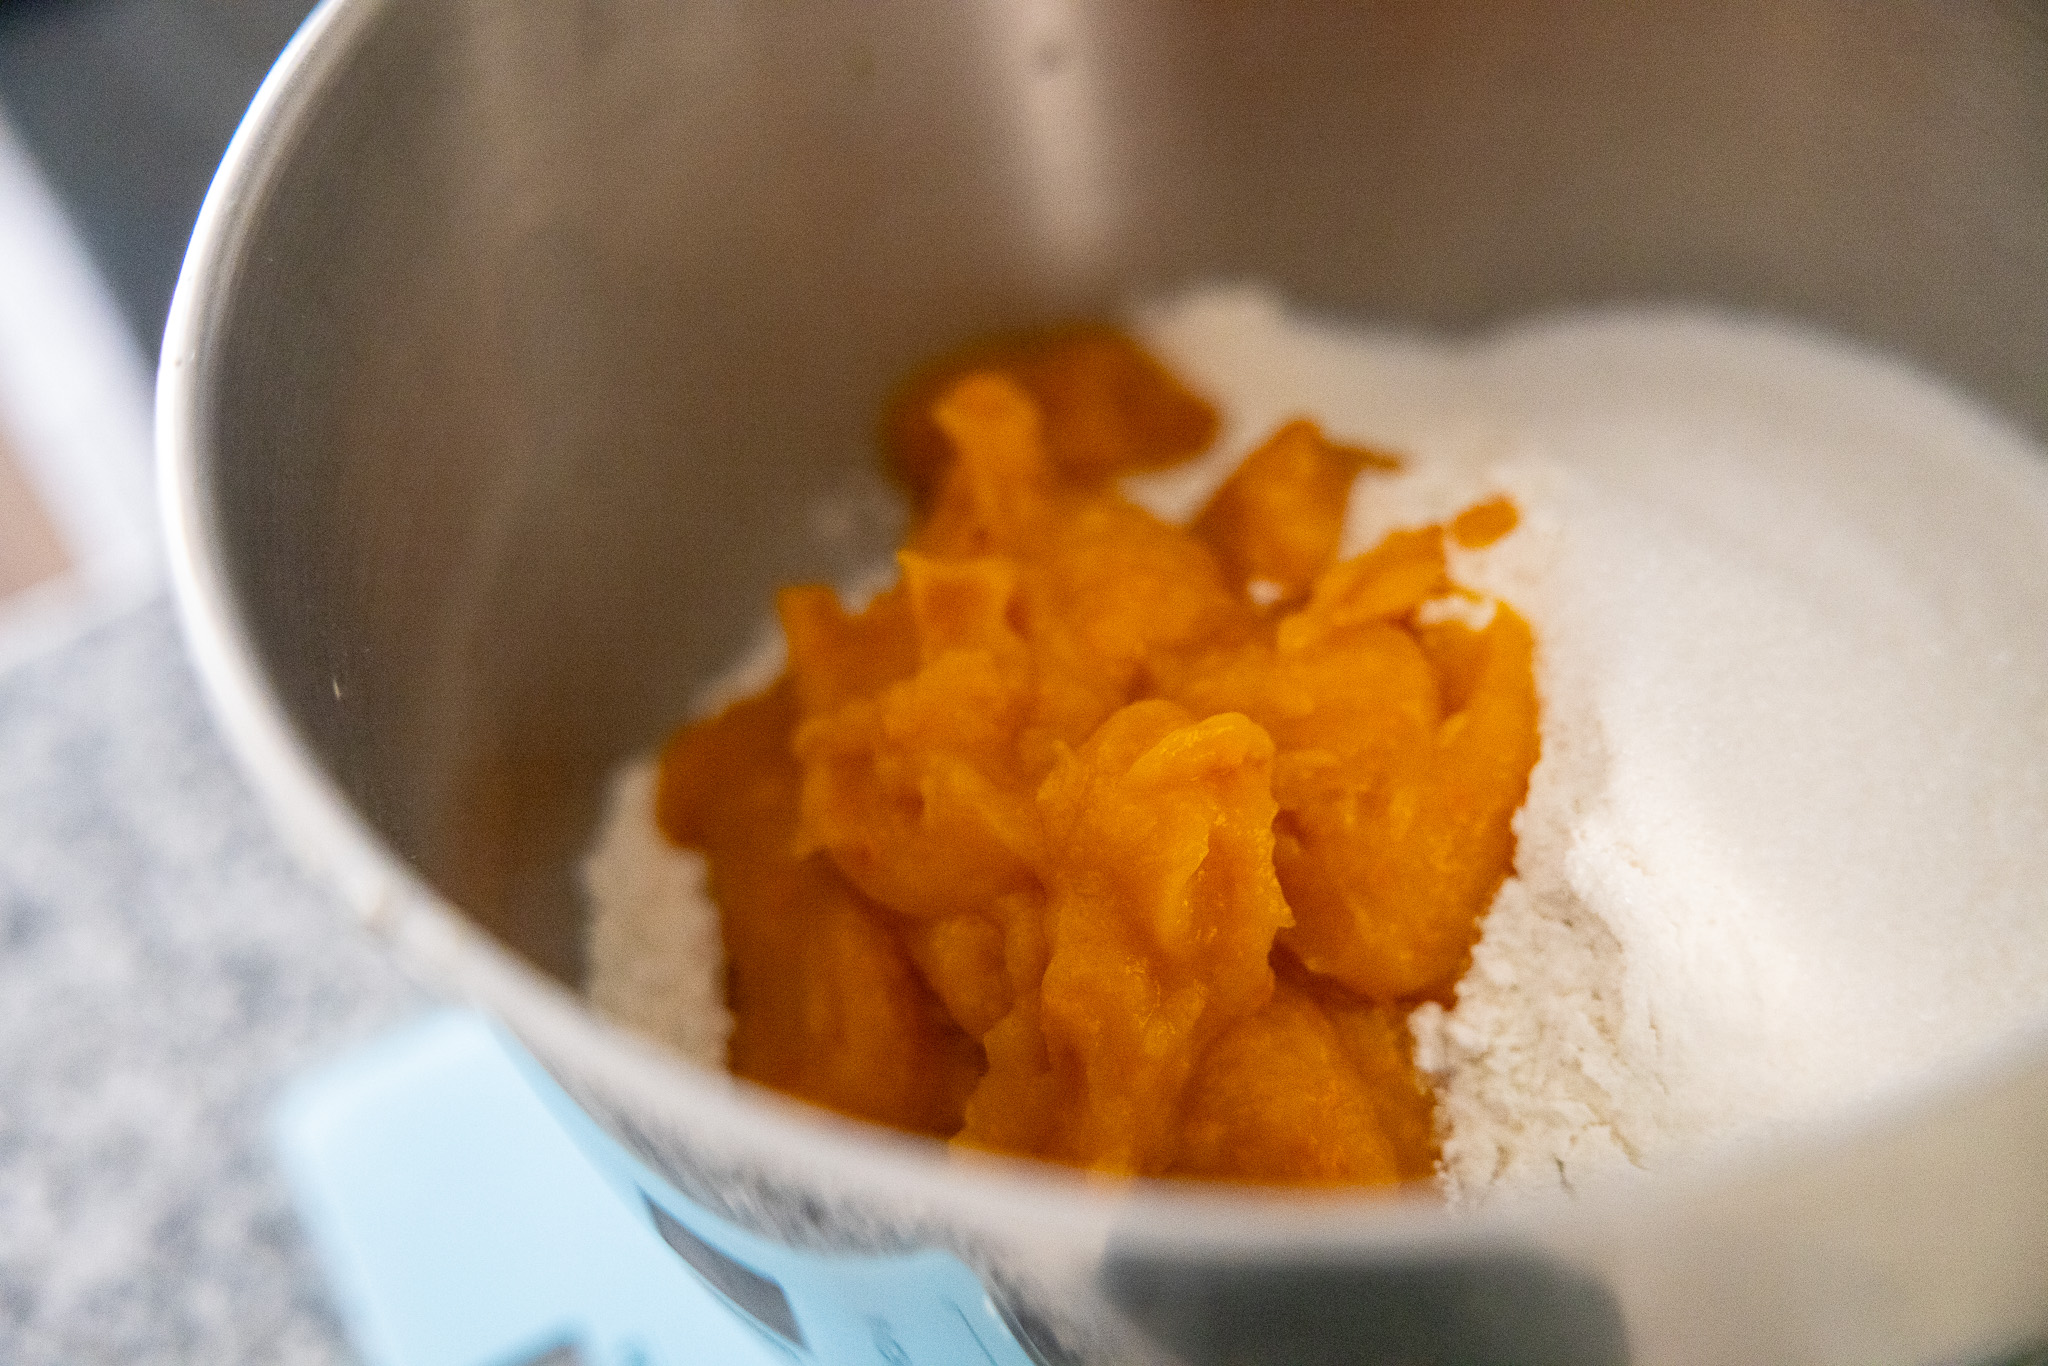
\includegraphics[width=\textwidth]{pumpkin-on-flour}
  \caption[Pumpkin puré]{A common mix-in technique is to replace some of
    the dough's water with another liquid. In this case, puréd pumpkin replaced
    some of the water. When adding puré to the dough only slowly add
    additional water as the puré slowly releases additional water to the
    dough.}%
\end{figure}

One approach to categorizing the mixins is to look at their respective shape.
However, the transition between these categories is somewhat fuzzy:

\begin{itemize}
  \item Liquids: Integrate homogeneously into the dough, may replace some of
      or all of the water. Examples: Milk, butter, oil, spinach juice, tomato
      juice, eggs
  \item Powders: Integrate homogeneously into the dough, may replace some of
      the flour. Examples: Milk powder, semolina, cocoa, spices
  \item Small bits: Individually visible in the final loaf, small enough to
      distribute somewhat evenly throughout the dough. Examples: Seeds (wheat
      berries, rye berries, poppy seeds, sesame, pumpkin seeds,
      flax seeds), whole spices (coriander)
  \item Chunks: Larger pieces that will only be present in the occasional bite
      when eating a slice of your bread. Examples: dried tomatoes, chunks of
      cheese, chunks of chocolate
\end{itemize}

Another categorization approach looks at the changes to the bread:

\begin{itemize}
  \item Flavor: Significantly changes the taste of the bread. Examples: rye
      flour, corn flour, spices, sugar.
  \item Color: Significantly changes the look of the bread. Examples: cocoa,
      squid ink, beetroot juice, tomato juice.
  \item Texture: Significantly changes the feeling in the mouth when eaten.
      Examples: Cheese (gummy), seeds (crunchy), olives (squishy chunks).
\end{itemize}

Many of the above-listed mix-ins can't be pinpointed to a single category. They
change multiple aspects of the final bread at the same time.

\begin{figure}[htb!]
  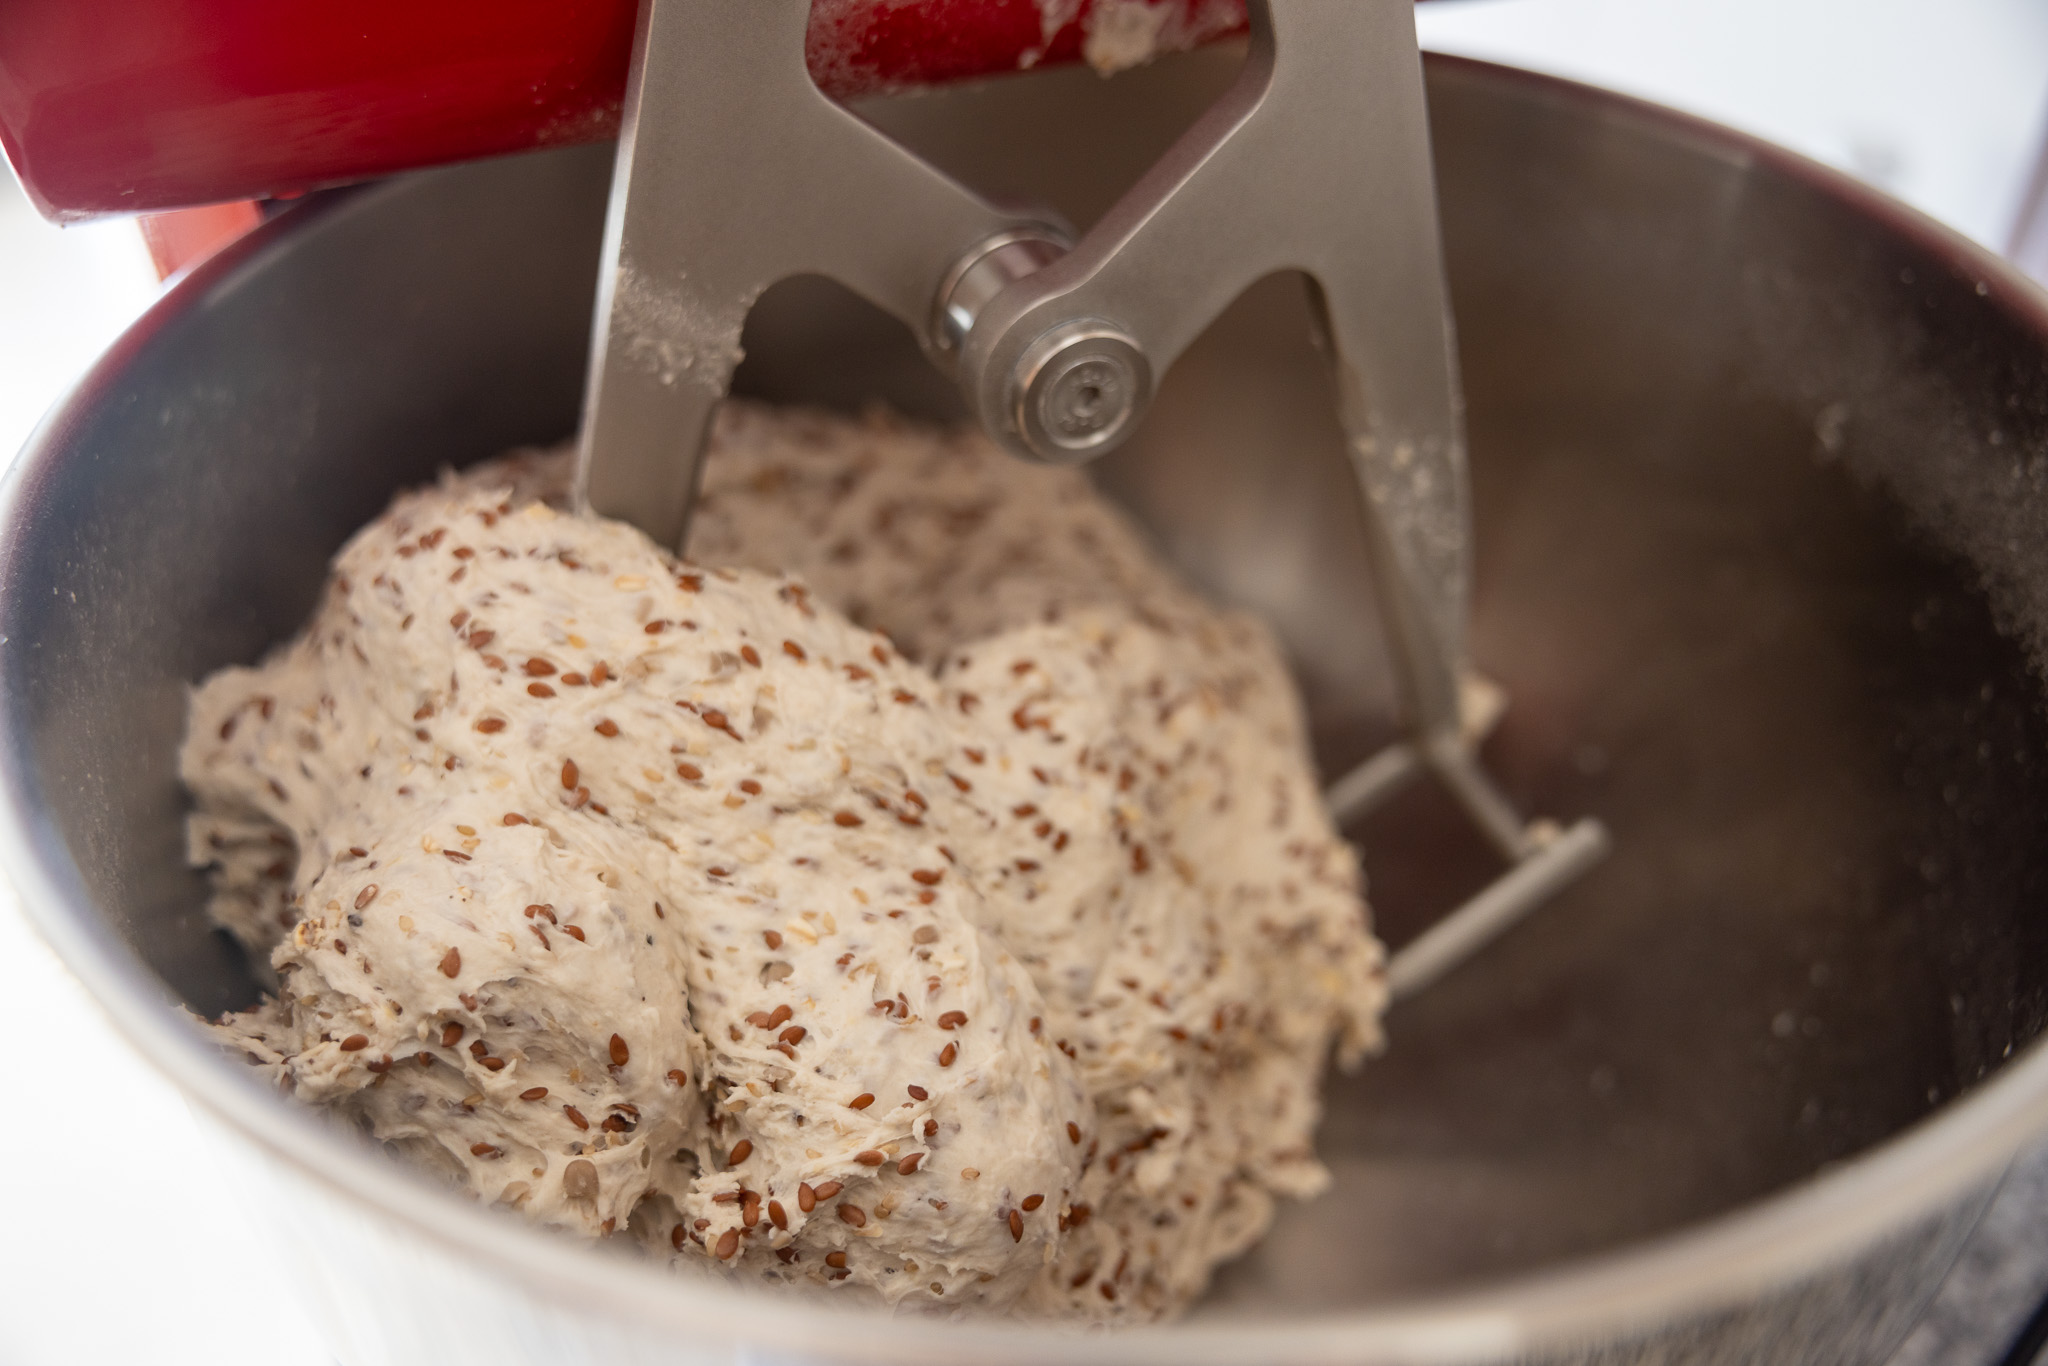
\includegraphics[width=\textwidth]{seeded-sourdough}
  \caption[Seeded sourdough]{In this case a combination of flax, sunflower and
    sesame was added to the dough. The seeds will slightly dehydrate the dough
    during fermentation and thus adding a bit more water (\qtyrange{1}{2}{\percent}) is advised.}%
\end{figure}

Mix-ins affect the structure of the dough. One aspect is the impact on
hydration. Some mix-ins absorb a lot of water when added to the dough, so you
have to increase the amount of water to achieve the same dough consistency.
The other impact is on the gluten network. Bits and chunks disrupt the gluten
network and may reduce oven spring during baking. All of this depends on the amount of mix-ins
used. A good rule of thumb is to add \qtyrange{10}{20}{\percent} of the amount
of flour in most mix-ins, reduced to around \qtyrange{1}{5}{\percent} of the
amount of flour for spices.

An important factor is also the mix-in's behavior during baking. Particularly
chunks may bake differently than dough, and either melt (cheese) leaving holes
inside, or char when peeking through the crust (\eg~vegetables). These
problems can be mitigated to some degree with the right preparation (\eg~chopping
into smaller pieces, soaking dry ingredients in water or oil first,
or squeezing out excess moisture).

\section{Examples}

The following is a list of common mix-ins and their peculiarities. They can be
combined depending on your preference.

\subsection{Flours}
These are powders. Usually, you want to just replace some fraction of the
regular bread flour. Different flours change the taste of the bread and
usually moderately affect the color.

\begin{figure}[htb!]
  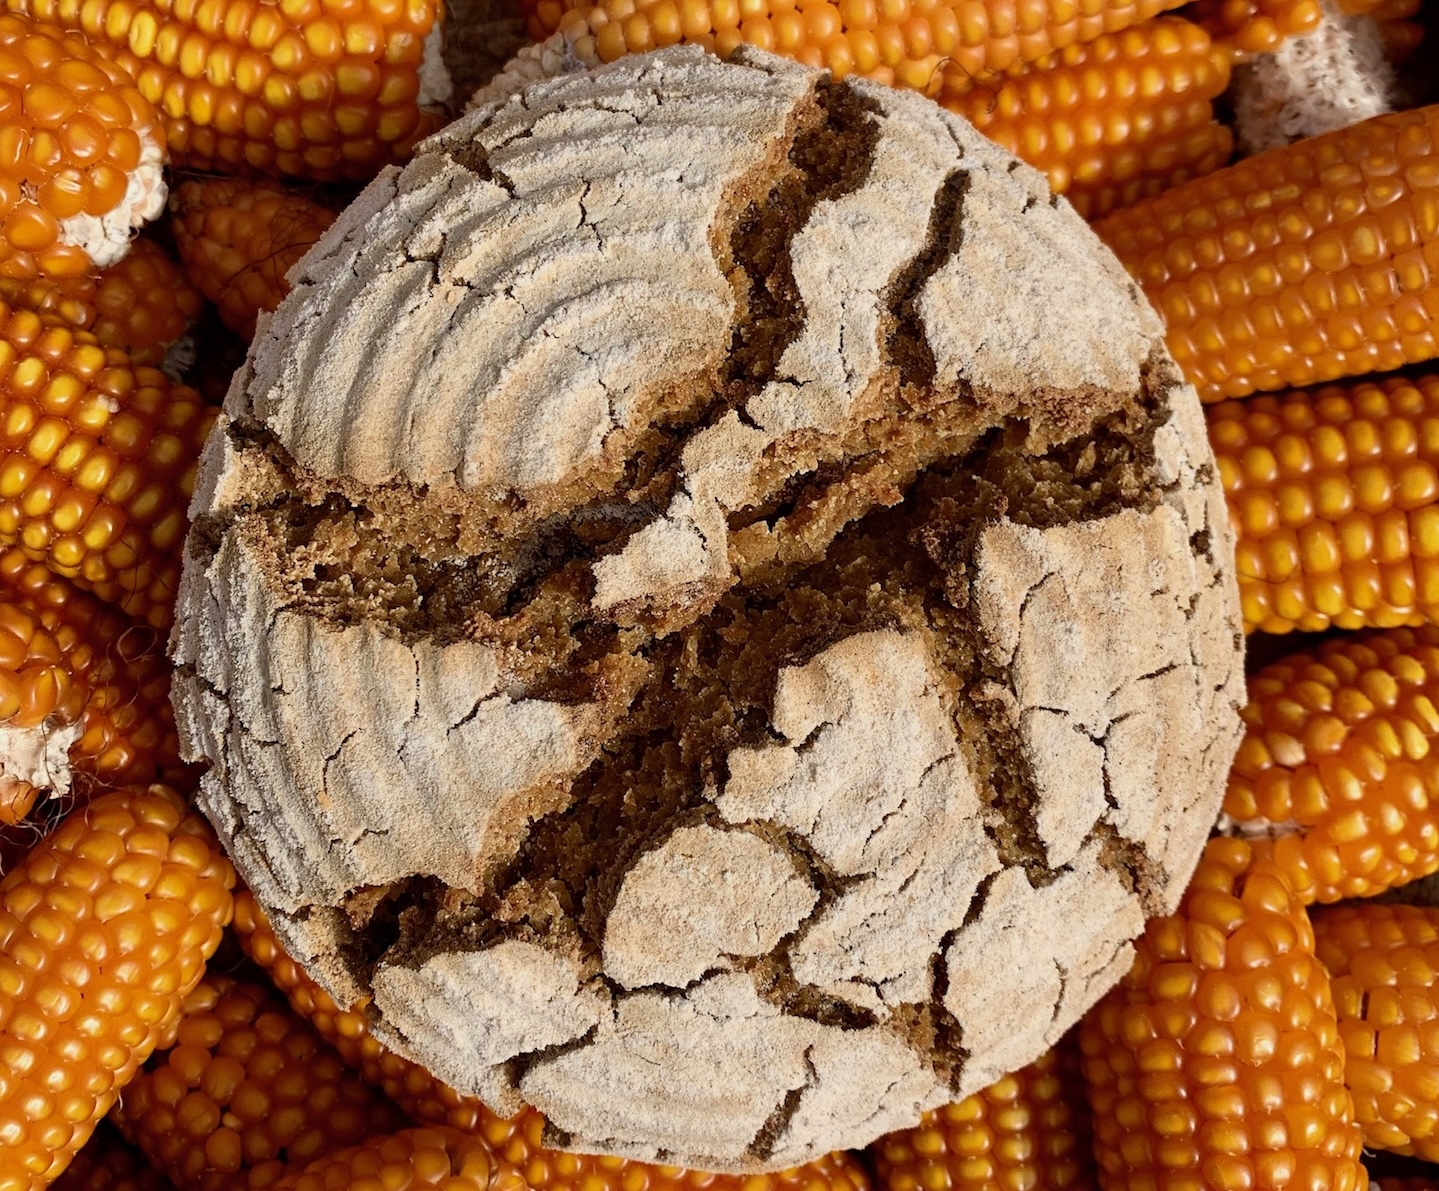
\includegraphics[width=\textwidth]{broa}
  \caption[Broa de milho]{Broa de milho is a traditional Portuguese bread
  made out of half rye and half corn flour.}%
\end{figure}

\begin{itemize}
  \item Whole wheat flour (substitute any amount, makes the bread taste more
      complex, nutty)
  \item Rye flour (very hearty, nutty, malty taste)
  \item Enzymatic malt (malty taste, improves enzymatic activity). The malt is
    a great addition when making quicker yeast-based doughs.
  \item Semolina (supports Mediterranean flavors)
  \item Cocoa (replace \qty{10}{\percent} of the flour for a black loaf, goes
      great with sweet toppings)
  \item Other non-wheat flours such as: Chickpea, corn, hemp, potato\dots{}
\end{itemize}

\subsection{Liquids}

Instead of using water, you can substitute it with a different liquid,
affecting taste and texture.

\begin{figure}[htb!]
  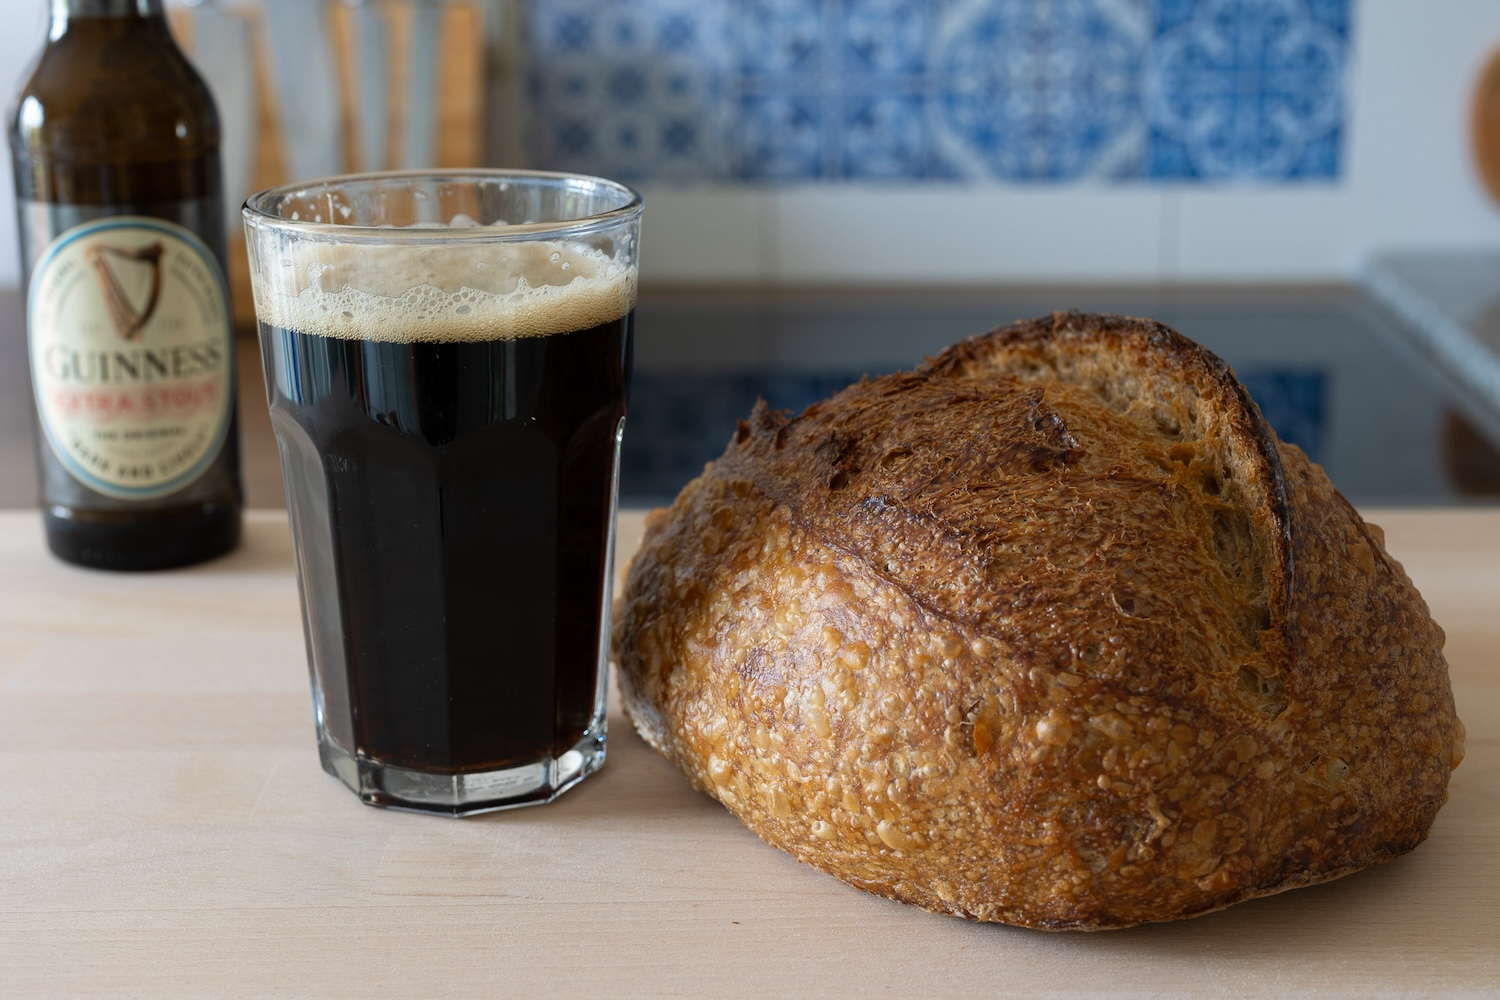
\includegraphics[width=\textwidth]{beer-bread}
  \caption[Stout beer bread]{Dark hearty stouts work excellently as a water replacement
  when making sourdough bread. The resulting loaf features a hearty malty taste}%
\end{figure}

\begin{itemize}
  \item Beer
  \item Butter
  \item Buttermilk
  \item Cereal milk (the leftover milk from eating cereals)
  \item Coffee
  \item Eggs
  \item Fruit/vegetable juices (also see Section~\ref{section:colors})
  \item Milk (for sweet, soft breads)
  \item Milk alternatives such as: Almond, oat, soy\dots{}
  \item Mashed potatoes
  \item Mashed sweet potatoes. Bolo do caco is a typical bread from Madeira,
    made from \qty{50}{\percent} wheat flour and \qty{50}{\percent} mashed potatoes.
  \item Olive oil (Mediterranean)
  \item Other mashed vegetables such as: Beets, pumpkin\dots{}
\end{itemize}

\subsection{Colors}%
\label{section:colors}
Some mix-ins will change the color and flavor of your bread. Common colorings
include:

\begin{itemize}
  \item Activated charcoal powder (black)
  \item Beetroot juice (red)
  \item Blueberry juice (blue)
  \item Blue butterfly pea flower powder (blue)
  \item Carrot juice (orange)
  \item Pear juice (pink)
  \item Spinach juice (green)
  \item Squid ink (black)
  \item Strawberry juice (red)
  \item Tomato juice (red)
\end{itemize}

\subsection{Seeds and nuts}
These are small bits, with some almost crossing into the chunk category. Some
seeds benefit from being boiled for about 10~minutes before adding them to the
dough.

\begin{figure}[htb!]
  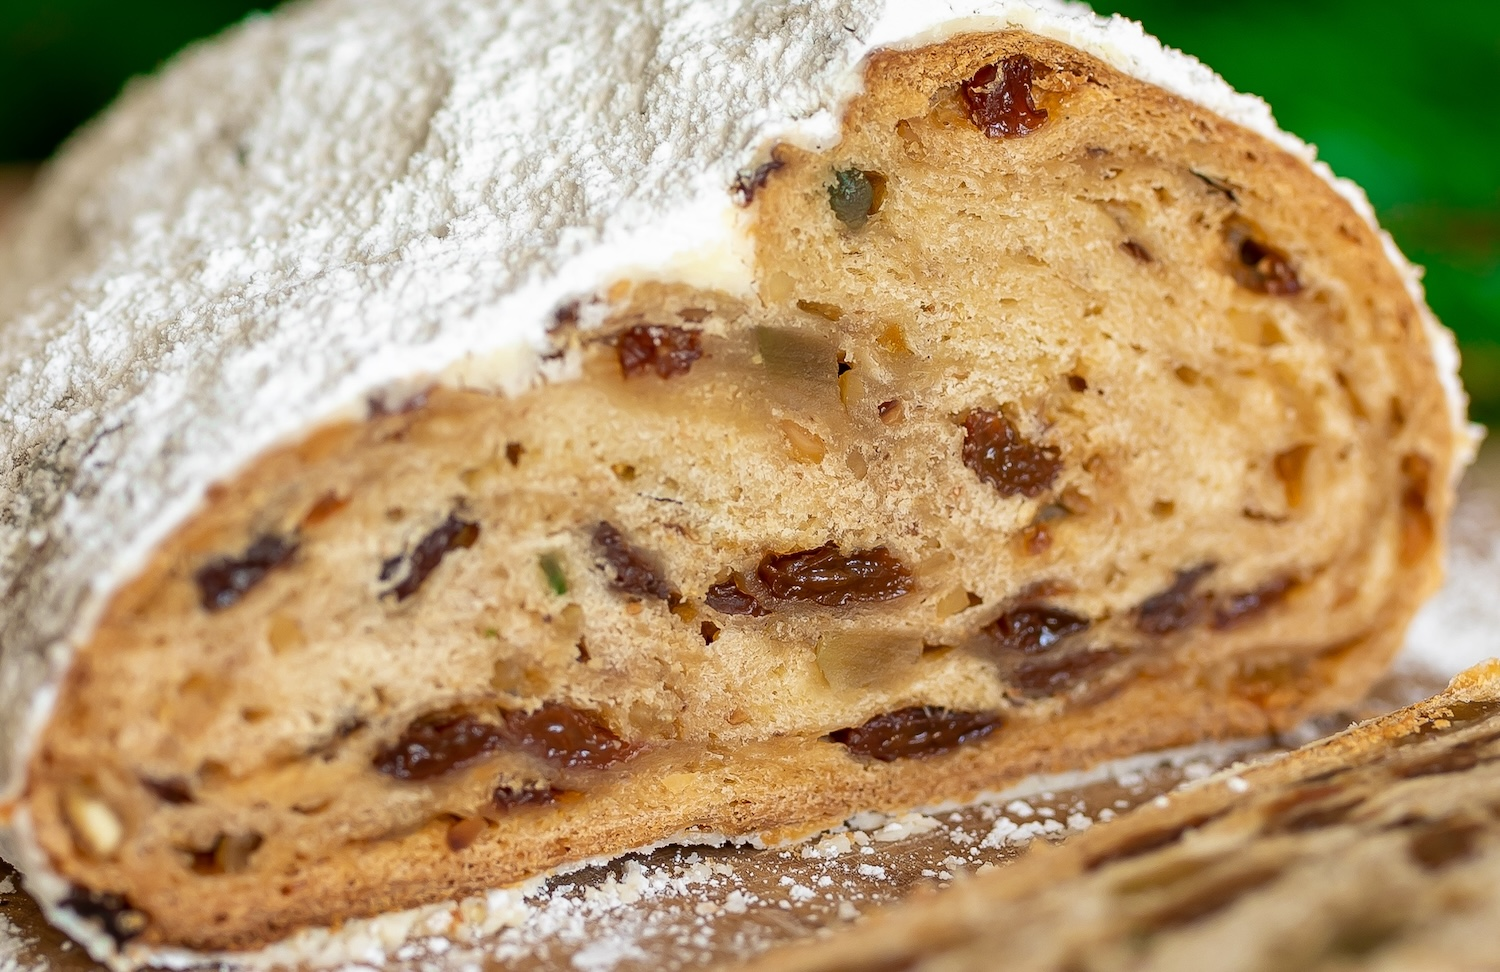
\includegraphics[width=\textwidth]{stollen-close-up}
  \caption[Stollen closeup]{The Stollen is a traditional German sweet Christmas
    bread featuring a variety of mix-ins. The dough typically contains candied lemon,
    candied orange, and raisins. The mix-ins are soaked in rum before being added to
    the dough. While the stollen matures after baking (up to \num{6} months) the candied ingredients release
    their aroma to the baked product.}%
\end{figure}

\begin{itemize}
  \item Cacao nibs
  \item Chia seed
  \item Chopped or whole nuts such as: Almonds, hazelnuts and walnuts
  \item Flaxseeds
  \item Hemp seed
  \item Poppy seed
  \item Pumpkin seed
  \item Sesame
  \item Sunflower seed
  \item Whole rye berries (boil 10 minutes)
  \item Whole wheat berries (boil 10 minutes)
\end{itemize}


\begin{figure}[htb!]
  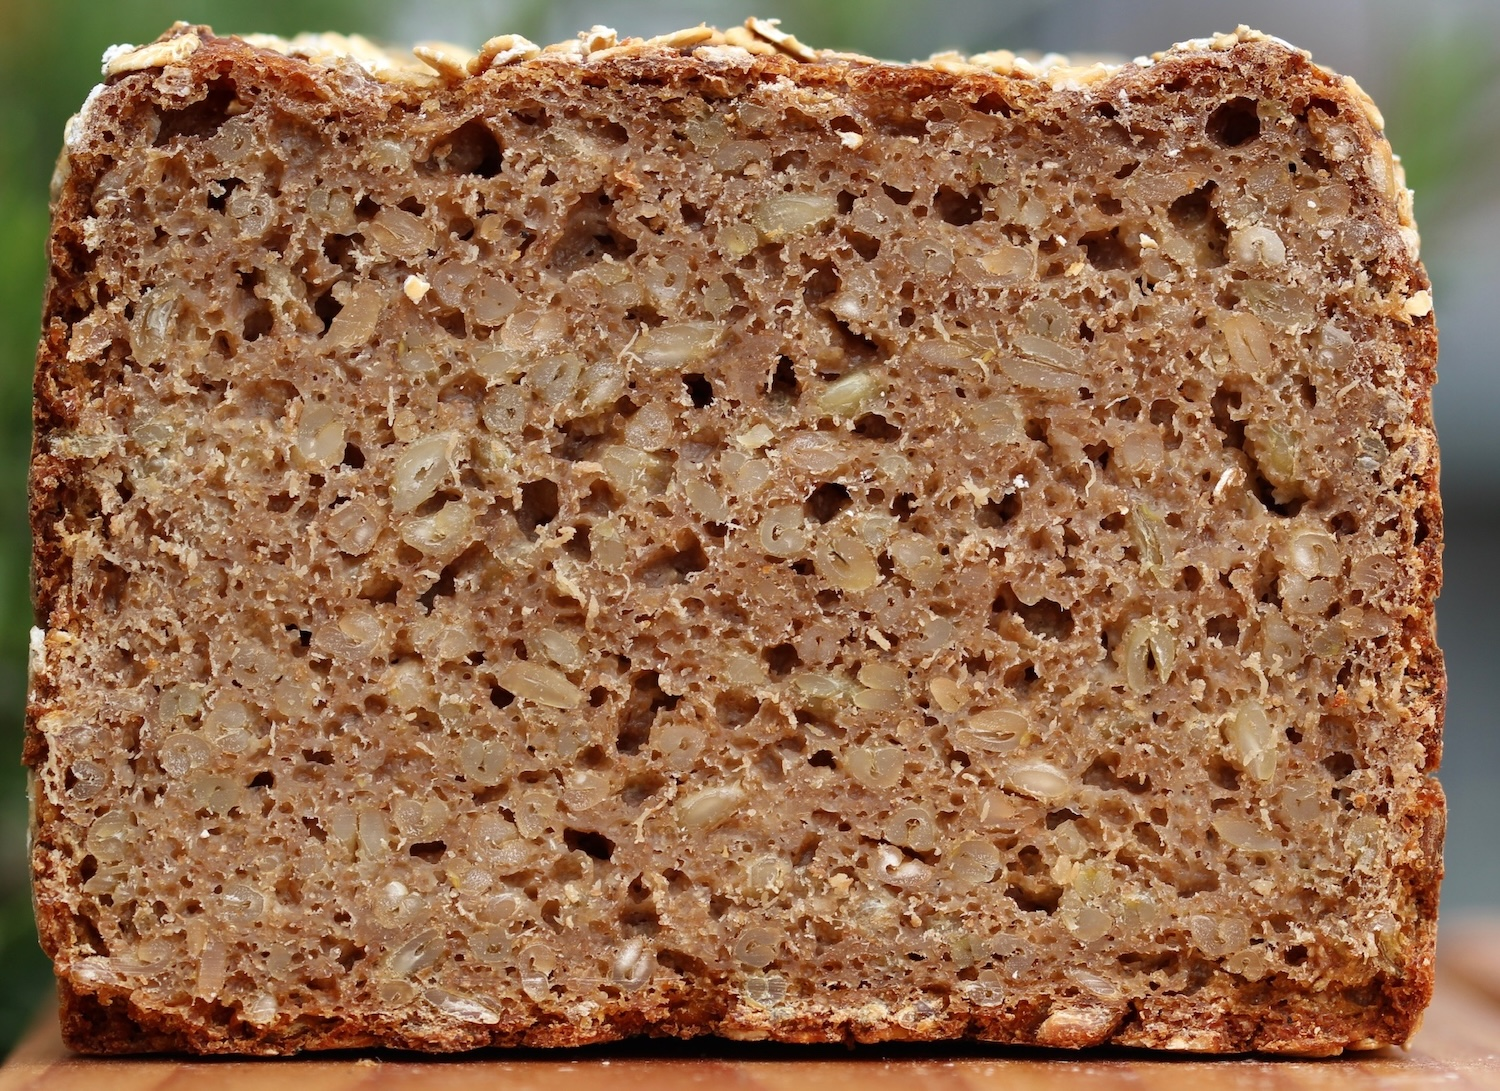
\includegraphics[width=\textwidth]{seeds-bread}
  \caption[Whole-rye with rye berries]{A sourdough bread made with half whole-rye flour and half rye berries. The
  berries are typically boiled for 10~minutes to allow them to soften a bit. When baking a loaf
  it is advised to use a thermometer to measure whether it is done baking. The final bread
  features a hearty tangy flavor and has a moist crumb.}%
\end{figure}

\subsection{Spices and flavor mix-ins}
These are mostly powders or small bits.

\begin{itemize}
  \item Blueberry skins (press through a sieve to remove juice), raw
      blueberries
  \item Browned onions
  \item Candied fruits such as: Lemon, orange, pineapple\dots{}
  \item Cinnamon
  \item Grated hard cheese such as: Gruyère, parmesan\dots{}
  \item Mediterranean herbs such as: Marjoram, oregano, rosemary, thyme\dots{}
  \item Miso
  \item Molasses
  \item Sugar
  \item Spices such as: Anise, fennel, cinnamon, coriander, cumin\dots{}
  \item Zests such as: Lime, Lemon, orange\dots{}
\end{itemize}

\subsection{Highlights}
Mostly chunks, that add a big contrast and flavorful highlight to the basic
bread. Usually, you want to use only one (or a maximum of two) of these. The suggestions
can often be complemented by some flavor or flour mix-in.

\begin{itemize}
  \item Chocolate chunks or drops
  \item Chunks of black garlic
  \item Chunks of cheese such as: Cheddar, feta\dots{}
  \item Cornflakes
  \item Dried fruits such as: Cranberries, dates, raisins\dots{}
  \item Olives
  \item Pickled pepperoni
  \item Sundried tomatoes (squeeze out the oil if using pickled ones, or soak
      dried ones in water)
\end{itemize}

\subsection{Combinations}
A few combinations where multiple mix-ins complement each other:

\begin{itemize}
  \item Butter and milk. Then add cinnamon and brown sugar before shaping
  \item Cheddar and pepperoni
  \item Cheddar and jalapeño
  \item Cocoa, cacao nibs, whole hazelnuts
  \item Cranberry and walnuts
  \item Semolina, Mediterranean herbs, olives, sundried tomatoes
  \item Tomato juice instead of water with \qty{20}{\percent} rye flour
\end{itemize}

\section{Techniques}

Adding mix-ins to the dough is just the simplest approach. Add the mix-ins
directly when you knead the dough. After the first kneading wait for 30 minutes to see
if the dough has enough or too much water. In the case of whole-soaked berries
(\eg~rye or wheat) chances are that the berries will release some water and make the dough
wetter. In this case, you will want to add a bit more flour to the dough to
compensate for the high hydration.

\subsection{Adding before shaping}

\begin{figure}[htb!]
  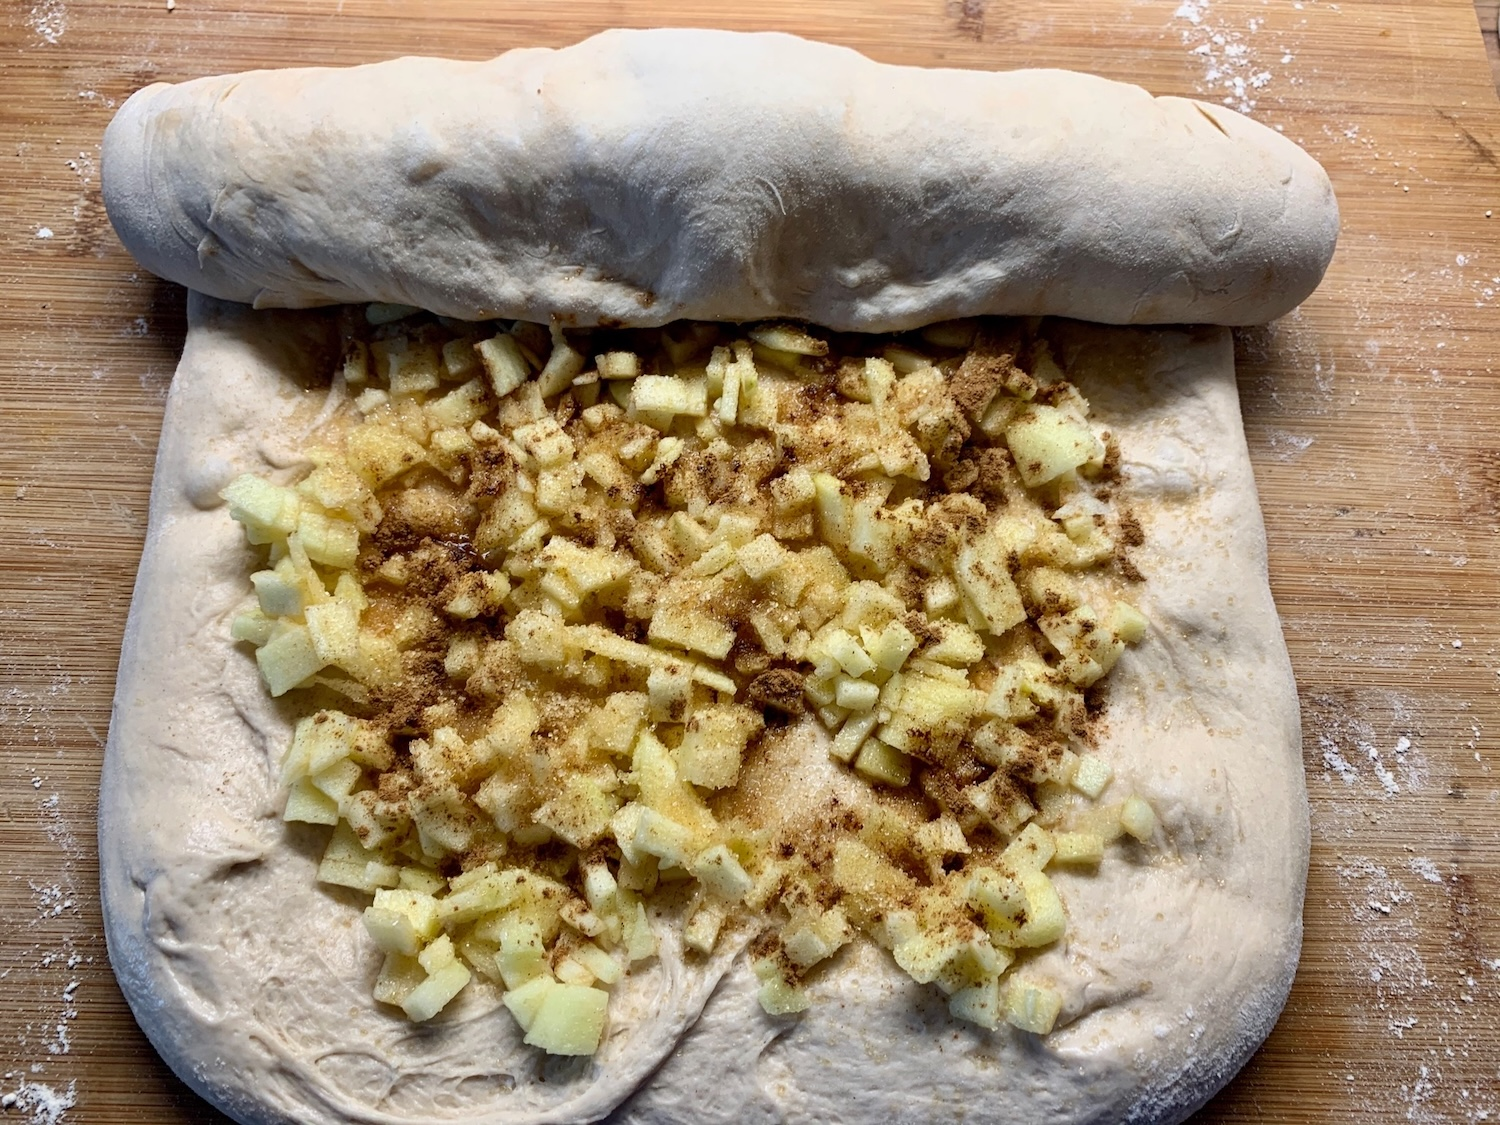
\includegraphics[width=\textwidth]{apple-swirl}
  \caption[Apple swirl buns]{A great technique is to add some of your mix-ins
  directly before shaping. In this case, a mixture of apples, cinnamon and brown
  sugar was applied. Proceed and roll the dough together. Afterward cut the roll
  into smaller pieces using a sharp knife, dough scraper or dental floss. Place
  each piece of dough next to each other in a greased bowl to allow them to be proofed.
  Proceed and bake as you would normally do. The benefit of this technique is that
  the mix-ins will not be fermented. This is typically required in the case of sugar
  since you want the final baked goods to feature sweetness. If included upon
  initial mixing most of the sugar would be fermented and the bread would not taste sweet.}%
\end{figure}

Another approach is to lay the dough out flat after the bulk fermentation.
Then using a spatula spread your ingredient over the flat dough. Continue with
your regular shaping and/or roll up the dough. When creating a roll you can
use a sharp knife to cut the dough, dental floss works great too. Afterward,
place the tiny swirls in a container to let them proof and become fluffier. This is an
excellent way to add sweet mixins as the microbes will not ferment them. When
adding sugar to the initial dough it will be fermented and the resulting dough
will not taste sweet (depending on the fermentation duration). This approach
is excellent for garlic/cheese rolls, garlic/herb rolls, and cinnamon rolls

\subsection{Covering the surface}

\begin{figure}[htb!]
  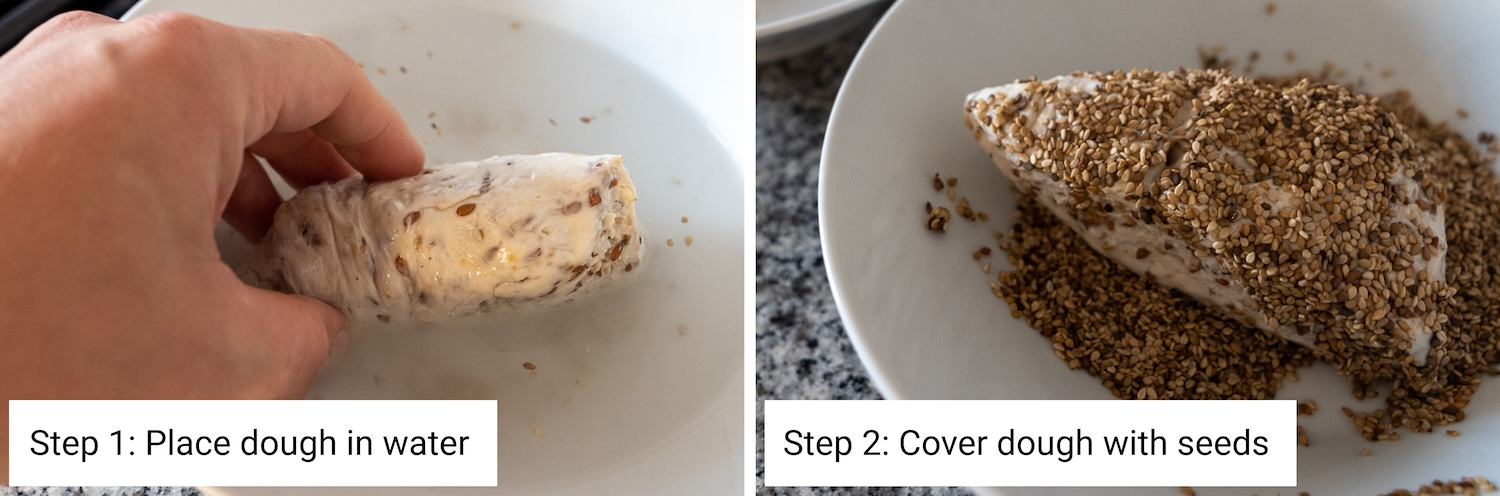
\includegraphics[width=\textwidth]{surface-seeds}
  \caption[Surface seeds]{These are chop buns which are created by chopping
    up a retarded dough into smaller pieces before baking. Then each piece of
    dough is quickly dumped in water and then rolled in a bowl of seeds.
    Afterward, the dough is directly baked in the preheated oven. These
    coverings add superb additional flavor and can be adjusted depending on
    your preference. I love adding a mixture of sunflower, flax, and
    sesame seeds.}%
\end{figure}

This works best for either powders or small bits. After shaping wrap your
coverings on the dough's surface. This works great too when covering your
banneton or loaf pan with seeds or oats. When using a loaf pan or banneton
these coverings also help to make the container stick less.

Another approach commonly used with buns is to wet the surface or dump the
dough in water. Afterward, dip the wetted piece of dough into your bowl of
mixins.  This does not work for all mix-ins, as some can't handle the high temperatures
during baking and char. Most commonly done with seeds (\eg~sesame, oats, flax-seed).

\subsection{Swirled colors}
Mix-ins that change the color of the dough bring the opportunity for even more
creativity by merging the dough before shaping.

Proceed and separate your base dough before adding a colorful ingredient. Bulk
ferment the dough in separate containers. Then Combine the two (or
more) differently colored doughs by laminating and stacking the colored sheets
of dough before the last folding, just before shaping. This way the colored
layers won't mix and the resulting dough will have differently colored and
tasting layers\footnote{I once made an experimental dough by merging a wheat,
rye, spelt and einkorn dough into a single dough. The resulting dough was
layered featuring different colors, textures, and flavors.}.


\chapter{Baking}%
\label{chapter:baking}
\begin{quoting}
Baking refers to the part of the process where you are loading your dough into
the oven\footnote{While some breads like flatbreads could also be baked on the
stove. This chapter focuses on the home oven.}.  Baking is typically done after
your dough has gone through the bulk fermentation and proofing stage.  This
chapter will review what happens to your dough during baking, as well as
several techniques used to improve the final result.
\end{quoting}

\section{The process of baking}
Once temperature starts to rise, the dough will go through several stages as
summarized in Table~\ref{tab:baking-stages}.  As the dough heats up, the water
and acids in your dough start to evaporate. When baking a gluten based dough,
the bubbles in your dough start to expand.  The dough starts to vertically
rise, this is called oven spring.  Your bread starts to build a crust of
gel-like consistency, the crust is still extensible and can be stretched.

\begin{table}[htp!]
    \centering
        \input{tables/table-baking-process-stages.tex}
        \caption[Stages of dough during baking]{The different stages that
            your dough undergoes during the baking process.}%
        \label{tab:baking-stages}
\end{table}

At around  \qty{60}{\degreeCelsius} (\qty{140}{\degF}) the microbes in your dough start to die.
There are rumors that until this happens the microbes produce
a lot of \ch{CO2}, resulting in the dough's expansion. However, this temperature
is reached quickly. Furthermore, stress makes the microbes
enter sporulation mode in order to focus on spreading genetics.
More research should be done here to validate or invalidate this
claim.

At  \qty{75}{\degreeCelsius} (\qty{167}{\degF}) the surface of your dough turns into a gel. It
holds together nicely but is still extensible. This gel is essential
for oven spring as it retains the gas inside your dough.

At around  \qty{100}{\degreeCelsius} (\qty{212}{\degF}) the water starts to evaporate out of your
dough. If this weren't the case, your dough would taste soggy and
doughy. The higher hydration your dough has, the more water your bread
still contains after the bake, changing its consistency.  As a result the
crumb is going to taste a bit more moist.

Another often undervalued step is the evaporation of acids.
At~\qty{118}{\degreeCelsius} (\qty{244}{\degF}) the acetic acid in your dough
starts to evaporate.
Shortly after at~\qty{122}{\degreeCelsius} (\qty{252}{\degF}) the lactic acid begins evaporating.
This is crucial to understand and it opens the door to many interesting
ways to influence your final bread's taste. As more and more water
begins to evaporate the acids in your dough become more concentrated.
There is less water but in relation you have more acids, therefore a shorter
bake will lead to a more tangy dough. The longer you bake the bread,
the more of the water evaporates, but also ultimately the acids will follow.
The longer you bake, the less sour your bread is going to be. By controlling
baking time you can influence which sourness level you would like to achieve.

It would be a very interesting experiment to bake a bread at different exact
temperatures. How would a bread taste with only evaporated water but
full acidity? What if you were to just completely get rid of the acetic
acid? How would the taste change?

\begin{figure}[!htb]
  \includegraphics[width=\textwidth]{baking-experiment-temperatures.png}
  \caption[Surface temperature for different steaming methods]{This
      chart shows how surface temperatures change using different steaming
      methods. In this case I~used a Dutch oven and an apple as dough
      replacement. All the apples were coming from the fridge. The temperature
      was measured using a barbecue thermometer.  The more steam, the faster
      the apple's surface temperature increases.}
\end{figure}

As the temperature increases further the crust thickens. The Maillard reaction
kicks in, deforming proteins and starches. The outside of your dough starts to
become browner and crisper, this process begins at
around~\qty{140}{\degreeCelsius} (\qty{284}{\degF})

Once the temperature increases even more to around~\qty{170}{\degreeCelsius}
(\qty{338}{\degF}),
the caramelization process begins, the remaining sugars and the microbes which
did not convert yet start to brown and darken. You can keep baking
for as long as you like to achieve the crust color that you
like\footnote{This really depends a lot on your personal preference.
Some people prefer a darker crust, others prefer a more pale crust.
It's better to build less crust than too much. You can always just
heat your bread in the oven one more time to continue building a
darker crust.}.

The best method to know that your dough is done is to take
the temperature of your dough, you can use a barbecue thermometer
to measure it. Once the core temperature is at around~\qty{92}{\degreeCelsius}
(\qty{197}{\degF}),
you can stop the baking process. This is typically not done though
as the crust hasn't been built yet\footnote{The thermometer is
especially important when using a large loaf pan. It is sometimes
very hard to judge from the outside if the dough is done. I~failed
many times and ended up having a semi baked dough.}.

Once your dough has finished baking, it is ready to eat: your
dough has turned into a bread. At this
point, your bread is sterile as the temperature was too hot for
for the microorganisms to survive\footnote{I~wonder though
if a starter culture could be grown again from a slice of bread.
Under heat stress the microorganisms begin sporulating. Maybe
some of the spores survive the baking process and could be reactivated
later? If this works, you could use any store bought sourdough
bread as a source for a new starter.}.

\section{The role of steam}
Steam is essential when baking as it helps to counter premature
crust building. During the first stage of the bake, the dough
increases in size as the water in your dough evaporates and pushes
the whole dough upwards.

Normally, under high heat a crust would form. Just like
if you were to bake vegetables in your home oven, at some point
they become darker and crisper. This is the same thing that
happens with your dough, and you want to delay this process
as long as possible until your dough no longer expands.
Expansion stops when most of the microbes have died and
the evaporating water no longer stays inside the alveoli.

The stronger the gluten network, the more gas can be retained
during the baking process. This gluten network at some point
loses its ability to contain gas as the temperature heats
up. The dough stops increasing in size. The steam plays
an important role as it condenses and evaporates on top
of your dough. The surface temperature is rapidly increasing
to around~\qty{75}{\degreeCelsius} (\qty{160}{\degF}). At this temperature the
gel starts to build, and is still extensible and allows expansion.
Without the steam, the dough would never enter the gel stage,
but instead directly go to the Maillard reaction zone. You
want your dough to stay in this gel stage as long as possible
to achieve maximum expansion\footnote{You can remove your
dough from the oven after 5~minutes to see the gel. You will notice
that it holds the dough's structure and it has a very interesting consistency.}.

\begin{figure}[!htb]
  \includegraphics[width=\textwidth]{baking-process-stage-2.jpg}
  \caption[Baking step~2, without steam]{The second stage of the bake is done
      without steam to build a thicker, darker crust.}
\end{figure}

When not steaming enough, you will notice that the scoring
incisions do not properly open up during the bake. They stay
closed as the dough is unable to push through the crust.
Another common sign, as you can see in Figure~\ref{fig:too-little-steam} is
that you have larger pockets of air towards the crust of your dough. As the
dough increases vertically, expansion is halted by the crust. The pockets
of air converge into larger pockets as the pressure increases.
This can also happen when you are baking at too high a temperature.

The more you steam, the softer your dough's crust is. You will never
enter the Maillard and caramelization stage. This
is the reason why the source of steam is removed
for the second stage of the bake. No more expansion can
happen and you can focus on building a crust. If you
would like a soft crust, you can steam your dough all the
way.

\begin{figure}[!htb]
  \includegraphics[width=\textwidth]{baking-too-hot}
  \caption[Bread baked too hot]{A submission by Karomizu showing a bread that
      has been baked at too high a temperature or with too little steam. Note
      the large pockets of air towards the crust. They are a typical
      indicator.}%
      \label{fig:too-little-steam}
\end{figure}

\section{Building up steam}
\begin{flowchart}[!htb]
\centering
  \begin{tikzpicture}[node distance = 4cm, auto]
  \node [start] (heat_oven) {Heat oven to  \qty{230}{\degreeCelsius} (\qty{446}{\degF}) for 30~minutes};
  \node [block, right of=heat_oven] (score_dough) {Score your dough};
  \node [decision, right of=score_dough, node distance=4cm] (decide_steam) {Choose your steaming method};
  \node [block, below of=decide_steam, node distance=3.5cm] (dutch_oven) {Dutch oven};
  \node [block, left of=dutch_oven] (inverted_tray_method) {Inverted tray method};
  \node [block, right of=dutch_oven] (steam_injection) {Steam injection oven};
  \node [block, below of=dutch_oven, node distance=3cm] (bake_30) {Bake dough for 30~minutes with steam};
  \node [block, below of=bake_30, node distance=3cm] (remove_steam) {Remove source of steam};
  \node [success, right of=remove_steam] (finish_baking) {Stop baking 10--30~minutes later depending on crust preference};
  \path [line] (heat_oven) -- (score_dough);
  \path [line] (score_dough) -- (decide_steam);
  \path [line] (decide_steam) -- (inverted_tray_method.north east);
  \path [line] (decide_steam) -- (dutch_oven);
  \path [line] (decide_steam) -- (steam_injection.north west);
  \path [line] (steam_injection.south west) -- (bake_30.north east);
  \path [line] (inverted_tray_method.south east) -- (bake_30.north west);
  \path [line] (dutch_oven) -- (bake_30);
  \path [line] (bake_30) -- (remove_steam);
  \path [line] (remove_steam) -- (finish_baking);
  \draw[BC, decoration=mirror] (remove_steam.south west) ++(0, -0.3) -- node[below=1em]{Building crust}(finish_baking.south east);
\end{tikzpicture}

  \caption[Different steaming methods]{A schematic visualization of the baking
      process using different sources of steam in a home oven.}%
  \label{fig:baking-process}
\end{flowchart}

\begin{figure}[!htb]
  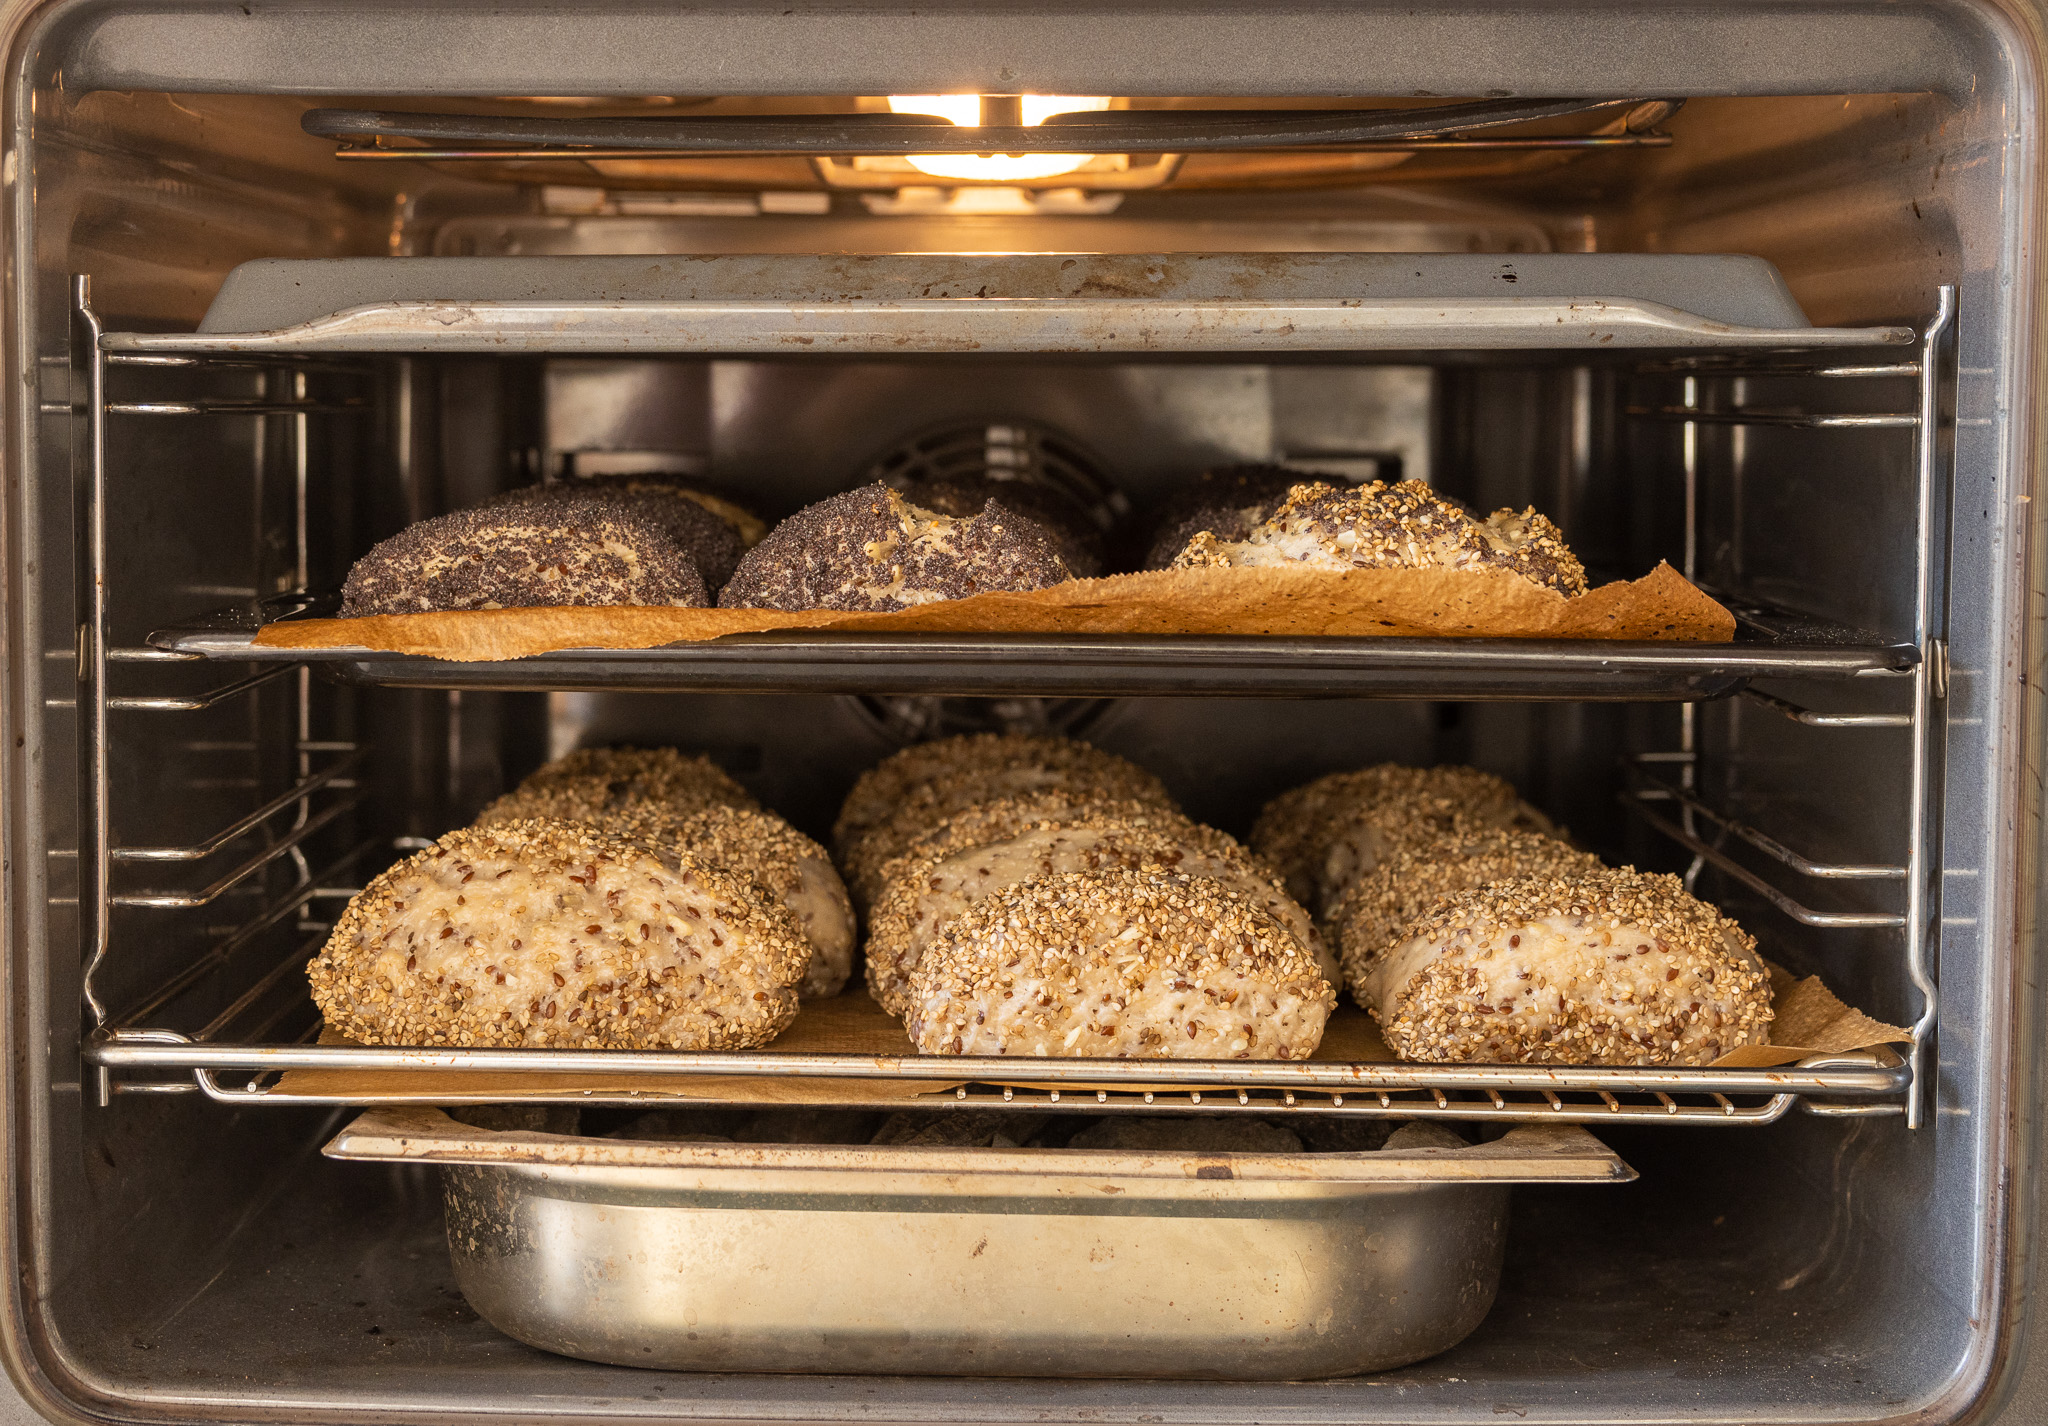
\includegraphics[width=\textwidth]{oven-example}
  \caption[Home oven baking example to maximize steam]{My default home oven setup. The tray of rocks
  and tray on top of the rolls greatly improve the steaming capabilities. This way the bread can
  rise more during the initial stage of the baking process.}
\end{figure}

\begin{figure}[!htb]
  \includegraphics[width=\textwidth]{baking-process-steam.jpg}
  \caption[Steam building with inverted tray]{How steam builds in your oven
      using the later described inverted tray method.}%
      \label{flc:inverted-tray}
\end{figure}

\subsection{Dutch ovens}

\begin{figure}[!htb]
  \includegraphics[width=\textwidth]{dutch-oven-example}
  \caption[Picture of dutch oven]{An example of a dutch oven. Some are also
      made out of enameled cast iron, others are made out of clay and some
      feature a glass lid.  They all work similarly by entrapping some of the
      steam created during the baking process. The steamy environment allows
      the bread to rise further and thus have more oven spring and feature a
      fluffier crumb.}%
\end{figure}

\begin{flowchart}[!htb]
\centering
  \begin{tikzpicture}[node distance = 3cm, auto]
  \node [start] (heat_oven) {Preheat DO to \qty{230}{\degreeCelsius} (\qty{446}{\degF}) for 30~minutes};
  \node [block, right of=heat_oven] (remove_oven) {Remove DO from oven };
  \node [block, right of=remove_oven] (open_load_dough) {Open DO \& load your dough};
  \node [block, right of=open_load_dough] (score) {Score your dough};
  \node [block, right of=score] (spritz) {Spritz dough with water};
  \node [block, below of=spritz] (close) {Close DO};
  \node [block, left of=close] (back_oven) {Place DO back in oven};
  \node [block, left of=back_oven] (bake) {Bake 30~minutes at \qty{230}{\degreeCelsius} (\qty{446}{\degF})};
  \node [decision, below right= 5cm and -1 cm of heat_oven]  (is_ready_check)
        {Core temperature \qty{92}{\degreeCelsius} (\qty{197}{\degF})?};
  \node [block, below of=is_ready_check, node distance=4cm] (wait_5_minutes) {Wait\\ 5 minutes};
  \node [block, right of=is_ready_check, node distance=4cm] (remove_do_lid) {Remove DO lid};
  \node [decision, right of=remove_do_lid, node distance=3.5cm] (dark_enough_decision) {Crust color dark enough?};
  \node [success, below of=dark_enough_decision, node distance=4cm] (finish_baking) {Bread is finished};
  \node [block, right of=dark_enough_decision, node distance=3.5cm] (bake_5_more_minutes) {Bake another 5~minutes};
  \path [line] (heat_oven) -- (remove_oven);
  \path [line] (remove_oven) -- (open_load_dough);
  \path [line] (open_load_dough) -- (score);
  \path [line] (score) -- (spritz);
  \path [line] (spritz) -- (close);
  \path [line] (close) -- (back_oven);
  \path [line] (back_oven) -- (bake);
  \path [line] (bake.west) -- node{} ++(-2, 0) -| (is_ready_check.north);
  \path [line] (is_ready_check) -- node{yes} (remove_do_lid);
  \path [line] (is_ready_check) -- node{no} (wait_5_minutes);
  \path [line] (wait_5_minutes.west) -- node{} ++(-1.5, 0) |- (is_ready_check.west);
  \path [line] (remove_do_lid) -- (dark_enough_decision);
  \path [line] (dark_enough_decision) -- node{yes} (finish_baking);
  \path [line] (dark_enough_decision) -- node{no} (bake_5_more_minutes);
  \path [line] (bake_5_more_minutes.east) -- node{} ++(1, 0) -- node{} ++(0, 2.3) -| (dark_enough_decision.north);
\end{tikzpicture}

  \caption[Baking process with a dutch oven]{A visualization of the baking
      process using a dutch oven (DO). The dough is steamed for the first half
      of the bake and then baked without cover for the second half of the
      bake. The desired darkness and thickness of the crust depends on your
      personal preference. Some bakers prefer a lighter crust and others a
      darker.}%
  \label{fig:dutch-oven-process}
\end{flowchart}

Dutch ovens are an ideal way to bake with a lot of
steam. They are not fully sealed. Regardless though,
as water evaporates from your dough, it will create a steamy
environment allowing your dough to rise. It
makes baking in a home oven very easy.

When using a Dutch oven, make sure to preheat it properly,
this way your dough will not stick to it. You can also
use additional semolina flour or parchment paper. Another
good trick is to spritz your dough with a bit of water.
To create more steam, you could also place a small ice cube
next to your main dough.

I~have been using a Dutch oven myself for a long time. They
have issues though. They are relatively heavy. It is dangerous
to operate hot cast iron ovens. Especially when working with steam,
you have to be very careful. Furthermore,
they are expensive to buy. If your Dutch oven is made out
of cast iron you have to season it from time to time. This takes
time.

The biggest disadvantage, though, is
capacity. You can only bake a single piece of bread at a time,
as the size of the Dutch oven is limited.
In many cases, it makes sense to bake multiple
loaves in one go. It makes the whole process more
efficient as you have to knead less per loaf. The time it
takes to make one loaf is significantly reduced on average. Furthermore,
you don't require as much energy. You don't have
to preheat your oven twice for each loaf.

An additional disadvantage of Dutch ovens is the
need to move very hot and heavy cast iron\footnote{%
  Some of them can weigh up to 10 kg. Moving them is quite
  a tedious exercise. Especially if the cast iron is
  heated you have to be very concise with your movements.
  Despite doing my best I have a few scars on my
  hands and arms from operating the Dutch ovens.
}.
You will need to be very careful and ideally use
heat-resilient gloves when touching your Dutch oven.

Furthermore, some of the Dutch ovens come at a hefty
price tag. Especially for new bakers buying a Dutch oven on
top of other tools can be quite a hefty investment. For
this reason, I advocate the inverted tray method visualized
in the next section. In case you do not own an oven consider trying
the simple flatbread recipe which is baked in a pan. Please
refer to Section~\ref{subsec:flat-bread-recipe} for more details.


\subsection{Inverted tray method}

The inverted tray method simulates a Dutch oven.
By placing another tray on top of your dough, the steam
created from the dough and water source stays
around your dough.

\begin{flowchart}[!htb]
\centering
  \begin{tikzpicture}[node distance = 3cm, auto]
  \node [start] (init) {Place water tray and stone in oven};
  \node [block, right of=init] (heat_oven) {Heat oven to  \qty{230}{\degreeCelsius} (\qty{446}{\degF}) for 30~minutes};
  \node [block, right of=heat_oven] (score_your_dough) {Score your dough};
  \node [block, right of=score_your_dough] (spritz) {Spritz your dough with water};
  \node [block, right of=spritz] (load_tray) {Place non-preheated inverted tray in oven};
  \node [block, below of=load_tray, node distance=4cm] (load_doughs) {Load doughs into oven};
  \node [block, left of=load_doughs, node distance=3cm] (load_water) {Place water in heated water tray};
  \node [block, left of=load_water, node distance=3cm] (bake) {Bake 30~minutes or until core temperature is  \qty{92}{\degreeCelsius} (\qty{197}{\degF})};
  \node [block, left of=bake, node distance=3cm] (remove_steam) {Remove steam source and top tray};
  \node [success, left of=remove_steam, node distance=3cm] (finish) {Bake at least another 10~minutes or until crust has your desired color};
  \path [line] (init) -- (heat_oven);
  \path [line] (heat_oven) -- (score_your_dough);
  \path [line] (score_your_dough) -- (spritz);
  \path [line] (spritz) -- (load_tray);
  \path [line] (load_tray) -- (load_doughs);
  \path [line] (load_doughs) -- (load_water);
  \path [line] (load_water) -- (bake);
  \path [line] (bake) -- (remove_steam);
  \path [line] (remove_steam) -- (finish);
\end{tikzpicture}

  \caption[Inverted tray baking process]{A schematic visualization the
  inverted tray baking method that works great for home ovens.}%
  \label{fig:inverted-tray-process}
\end{flowchart}


The biggest advantage of this method compared to the
Dutch oven is scalability. You can bake multiple loaves
at the same time. In my case that is around 2 freestanding
loaves and 4 loaves in a loaf pan.

For the inverted tray you will need the following tools:
\begin{itemize}
\item 2 trays
\item 1 heat resistant bowl
\item Boiling water
\item Oven gloves
\item (Optional) Parchment paper
\end{itemize}

\begin{figure}[!htb]
  \includegraphics[width=\textwidth]{baking-example.jpg}
  \caption{My home oven setup.}
\end{figure}

These are the steps to follow with the inverted tray method:
\begin{enumerate}
\item Preheat the oven to around  \qty{230}{\degreeCelsius} (\qty{446}{\degF}) and
preheat one of the trays.
\item Bring water to boil.
\item Place your loaves on a piece of parchment paper. You
can also place each on a tiny piece of parchment paper.
This makes loading the dough easier. If you don't
have it or don't want to use it, you can opt for
semolina flour. It helps to make the tray nonstick.
\item Take out your hot tray and place it
on a cooling rack or on something else that
is heat resistant.
\item Score your doughs.
\item Place your doughs on the hot tray.
\item Place the cold tray in your oven in an inverted position.
\item Move your hot tray including the loaves back
to the oven.
\item Place the boiling water in the heat-resistant
water bowl. I~have added rocks to it, as it helps
to improve the steam even further. This is optional.
\item Close the oven.
\item After 30~minutes remove the top tray. Also remove the bowl with water.
\item Finish baking your bread until you have reached your desired
crust color. In my case this is another 15--25~minutes typically.
\end{enumerate}

\section{Conclusions}

\begin{table}[!htb]
    \centering
        \input{tables/table-oven-baking-overview.tex}
        \caption[Different oven types]{An overview of different oven types and their
            different baking methods.}
\end{table}

Depending on your home oven, a different method
of steaming may be used. Generally most ovens
are made to vent out most of the steam during the
bake. They are typically not fully closed. During
baking you want to dry out whatever you are baking.
This is ideal if you are roasting vegetables and
want them to dry out. For baking though, this is
highly problematic. As described earlier, you
want there to be as much steam as possible.

If you are using a gas-based oven, the only option
is to utilize a Dutch oven. The same is true when you
are using a convection oven with a fan that
cannot be disabled. When using a convection
oven with a fan that can be turned off, you can
opt to use the cost-efficient inverted tray
method.

If you are in the luxurious
position of owning a steam oven, things are easier.
Just activate the steam function and you are
good to go. Placing an additional tray on top of your
dough during the bake helps to bake with indirect
heat. You remain in the gel zone longer and
will experience more oven spring.


\chapter{Storing bread}%
\label{chapter:storing-bread}
\begin{quoting}
In this chapter you will discuss different methods of storing your bread, each
with their own pro and cons.  This way your bread can be best enjoyed at a
later time.
\end{quoting}

A summary can be found in Table~\ref{table:bread-storage}, with details and
explanation in th rest of this chapter.
\begin{table}[!htb]
    \centering
        \def\arraystretch{1.6}
\begin{tabular}{@{}p{0.23\textwidth}p{0.33\textwidth}p{0.33\textwidth}@{}}
\toprule
\textbf{Method}     & \textbf{Advantages}            & \textbf{Disadvantages}       \\
\midrule
Room temperature                          & The easiest option. Best for bread that is eaten within a day.
                                            Crust typically stays crisp when humidity not too high.
                                          & Bread dries out very quickly.\\

Room temperature in airtight container    & Good for up to a week.
                                          & Bread needs to be toasted for crust to become crisp again. Catches mold more quickly\\

Fridge                                    & Bread stays good for weeks. Can dry out a little bit when not using air-tight container.
                                          & Bread needs to be toasted. Requires fridge and energy.\\

Freezer                                   & Bread stays good for years.
                                          & Requires thawing and then toasting. Requires freezer and energy.\\
\bottomrule
\end{tabular}

        \caption[Options to store bread]{A table visualizing the advantages
            and disadvantages of different bread storing options.}%
        \label{table:bread-storage}
\end{table}

\section{Room temperature}

The most common method is to store your bread
at room temperature. After taking a slice of bread,
store your bread with the crumb facing side
downwards.

This method works great if you want to eat
your bread within a day. The crust stays
crisp and does not become soft\footnote{The higher the humidity in your room,
    the faster the crust will become soft.}.
The biggest downside to this method is that
the bread becomes hard quickly. As time progresses,
more and more water evaporates from your dough's
crumb. Ultimately, the bread will become very hard
and impossible to eat. The more water you use
to make the bread, the longer the bread stays good.
A low-hydration recipe can dry out after 1--2 days;
a high-hydration bread needs 3--4 days to dry out.

Once your bread has dried out, you can run it under
tap water for around 10 to 15~seconds.
This water bath allows the
crumb's starch to absorb a lot of water. Proceed and
bake your bread again in the oven. The resulting loaf
will be almost as good as new again.

Another option for dried-out bread is to use it
to make breadcrumbs. These bread crumbs can be mixed
into subsequent loaves. They can also be used as
base ingredients for other recipes such as \emph{Knödel}\footnote{\emph{Knödel} is an
    Austrian dish that uses old bread as a basis.
  Breadcrumbs and day-old bread are mixed with eggs, and sometimes
  spinach or ham are added. The batter is then boiled in salty water.
}.

\section{Room temperature in a container}

Just like the previous option, you can also store your
bread inside a container. This could be a paper bag,
a plastic bag, or a bread storage box. The paper bag and
most bread boxes are not fully sealed, allowing some of
the air to diffuse out of the container. This also means that
the bread will slightly dry out.

When using a sealed bag such as a plastic bag, the bread
will retain a lot of moisture. The bread will stay good
for a longer period. However, at the same time, the crust
will also lose its crispness. Some of the water diffuses
into the bag and is then re-absorbed by the crust. If
you want the crisp crust, the best option is to toast your
bread.

Another problem with storage containers is natural
mold contamination. The moment your bread is taken out of
the oven it starts being contaminated with aerial mold spores.
The spores are microscopically small and are everywhere.
The mold spores grow best in a humid environment. By placing
your dough in a container you have created a mold paradise.
A plain yeast-based dough will start to mold within a few days
like this. The sourdough-based bread stays good
for a longer period as the acidity is a natural mold
inhibitor.

\section{Fridge}

In my own experience storing bread inside the fridge
works well as long as you use a sealed container, even if some
sources say that the bread dries out inside of the
fridge~\cite{storing+bread}. Supposedly the fridge
encourages liquid from the crumb to migrate to the bread's surface.

In my experience though, the trick is to use a sealable
container. With a sealable ziplock bag,
the excess humidity will stay in the bag and ensures
that the bread does not dry out as quickly. At room
temperature, this would cause your bread to mold. At
lower temperatures, the bread can stay good like this for
weeks. The crust however, will lose its crispness and
thus toasting is advised.

\section{Freezing}

Another great option for long-term storage is to use
your freezer. Slice up the whole loaf and create portions
that you can consume within a day. Store each portion
in a separate container and place them inside your
freezer.

When you want to eat fresh bread, open one of the containers
in the morning and allow the bread to thaw over a few
hours. This is needed so you can easily separate the frozen-together
slices. Toast the slices in your toaster
or bake them in the oven until they have the crispness
that you like.

This option is great for very long-term storage. Personally
I~like having a few slices of bread frozen as an emergency
backup when I~have had no time to bake.

A 2008 study hints that there might be some health
benefits to freezing and toasting your bread. By doing so
the starch molecules could become more resistant to digestion
and thus lower your body's blood sugar
response by almost 40\%~\cite{freezing+toasting+bread}.

\chapter{Troubleshooting}
\input{troubleshooting/misc-translated}

\backmatter
\chapter{Glossary}%
\label{ch:Glossary}

\begin{quoting}
This glossary provides definitions and explanations for terms frequently
used in bread making. Understanding these terms is essential for both
novice and experienced bakers aiming to master the art and science of
bread making. The glossary is arranged alphabetically for easy reference.
\end{quoting}

\begin{description}

\item[Acetic Acid] A type of organic acid produced by hetero fermentative lactic
acid bacteria and acetic acid bacteria during fermentation. It gives sourdough bread
its characteristic tangy flavor and helps to preserve the bread by lowering its pH.
The flavor of acetic acid has a more vinegary profile.

\item[Aliquot jar] A small piece of dough extracted after creating initial
dough strength.  The aliquot jar is used to monitor the dough's fermentation progress.
It's important to ensure the dough's water temperature in the aliquot matches
your room temperature for accurate readings. Be mindful that the aliquot
jar may not be as effective if there are significant temperature
fluctuations in your kitchen. This is because the small dough sample in
the aliquot can heat up or cool down faster than the main dough mass,
potentially impairing its ability to accurately monitor fermentation.
It's crucial to use a cylindrical-shaped aliquot container to properly judge
the dough's size increase.

\item[All Purpose Flour] A general flour that’s balanced to make breads and also
cakes. In Germany this is type~550.

\item[Alpha-amylase] A type of amylase that breaks down starch molecules into
shorter fragments, producing maltose and some glucose.

\item[Alveograph] A device used primarily in the evaluation of wheat flour's
baking quality. The alveograph assesses the dough's rheological properties,
particularly its extensibility and resistance to extension, by inflating a piece
of dough like a balloon until it bursts. The resulting chart, or \emph{alveogram},
displays a curve that represents the balance between the dough's elasticity and
extensibility. Specific parameters derived from the curve, such as the P (pressure
required to inflate the dough) and L (extensibility of the dough), provide invaluable
insights to bakers and millers regarding the flour's potential performance in
bread-making. By analyzing the alveogram, professionals can make informed decisions
about the suitability of a flour for certain baking applications, as well as
potential blending needs with other flours.

\item[Alveoli] (singular Alveolus) The little pockets that form the crumb,
formed by the gluten matrix trapping carbon dioxide.

\item[Amylase] An enzyme that breaks down starches into simpler sugars, facilitating
the fermentation process in beer and bread making. When making beer the temperature
of the brew is kept for extended periods at certain temperatures to ensure that most
starches are broken down to sugars. These sugars are then consumed by the microbes
during the fermentation process.

\item[Autolyse] A process where flour and water are mixed and then left to rest
before adding other ingredients. This activates enzymes such as amylase and protease.
By doing so the bulk fermentation time is shortened and the final loaf will have
better properties. The browning of the loaf becomes better and the crumb fluffier.
An autolyse is recommended when using a high percentage of starter to inoculate the
dough (>~\SI{20}{\percent}). An alternative easier approach can be the fermentolyse.

\item[Bacteria] Unicellular microorganisms that exist in diverse forms and
habitats. They play crucial roles in various natural processes, especially in food
preparation like sourdough fermentation. Lactic and acetic acid bacteria, in particular,
are pivotal in the sourdough process, contributing to its distinct taste and texture.
Some bacteria are beneficial, aiding in digestion or producing vitamins, while others
can be harmful and cause diseases.

\item[Baker’s Math] Baker’s math is a ratio based system of sharing recipes,
making them easily scalable. It’s based on the total weight of the flour in a formula,
where each ingredients weight is divided by the flours weight to give a percentage.
For \SI{500}{\gram} of flour you could be using \SI{60}{\percent} of water (\SI{300}{\gram}),
\SI{10}{\percent} of starter (\SI{50}{\gram}) and \SI{2}{\percent} of salt (\SI{10}{\gram}).

\item[Baker’s percentage] See Baker’s math.

\item[Baking] The final, transformative step in bread making wherein dough is
exposed to high temperatures, causing a series of chemical and physical reactions
that result in a finished loaf of bread. During the baking stage:

\begin{enumerate}
\item \emph{Yeast Activity \& Oven Spring:} In the initial phase of baking, the
temperature inside the dough rises, increasing yeast activity. This results in rapid
carbon dioxide production, leading to what bakers refer to as \emph{oven spring}, or the
rapid rise of the loaf.

\item \emph{Protein Coagulation:}  As the temperature continues to climb, the proteins
in the dough, primarily gluten, begin to coagulate or set, which gives the bread its
structure.

\item \emph{Starch Gelatinization:}  Starches absorb water and swell, eventually
gelatinizing. This process contributes to the crumb structure of the bread.

\item \emph{Caramelization \& Maillard Reaction:}  The crust of the bread browns due
to two primary reactions: caramelization of sugars and the Maillard reaction between
amino acids and reducing sugars. This not only affects the appearance but also imparts
a distinctive flavor and aroma to the bread.

\item \emph{Evaporation of Acids:} Some acids produced during fermentation evaporate at
certain temperatures during baking. This evaporation can influence the final flavor
profile of the bread, making it less tangy than the unbaked dough. By extending the
baking time the acids become less concentrated and the dough can lose some of its tang.

\item \emph{Moisture Evaporation:} Water in the dough turns to steam and begins to
evaporate. The steam contributes to the oven spring and also helps in gelatinizing
the starches.

\item \emph{Crust Formation:} The outer layer of the dough dries out and hardens to
form a crust, which acts as a protective barrier, keeping the inner crumb moist.
\end{enumerate}

\item[Banneton] A wicker basket used to shape and support dough during its final
proof. The bannetons are typically made out of rattan or wood pulp. An alternative
DIY solution is to use a bowl with a kitchen towel inside. While resting inside of
the banneton the dough’s surface dries out and becomes easier to score before baking.

\item[Bassinage method] A bread making technique involving the staged addition of water
to the dough. Initially, the dough is mixed to a lower hydration level,
allowing gluten bonds to form more effectively. Once these gluten structures
are established, additional water is gradually incorporated through further
kneading. This method enhances the dough's extensibility, especially beneficial
when working with lower-gluten flours. By employing the bassinage method,
bakers can achieve a dough that is both strong and extensible.

\item[Bench Rest] A short resting period given to the dough after preshaping
allowing the gluten to relax a little bit and making shaping easier. Most people
bench rest for 10 minutes up to an hour. The bench rest becomes especially important
when making pizza doughs. Without an extended bench rest the dough is too elastic and
can not be shaped.

\item[Beta-amylase] An enzyme that further breaks down the starch fragments
produced by alpha-amylase into maltose.

\item[Bread Flour] A flour that is perfect for sourdough bread making. It features
a higher amount of gluten and can thus ferment for a longer period of time.

\item[Brühstück] A German baking technique similar to a scald. It translates as
\emph{boil piece}. Hot or boiling water is poured over whole grain flour or crushed grains,
then cooled and mixed with the main dough. This process helps in moisture retention
and can enhance the flavor and texture of the final bread. Also see \emph{scald}.

\item[Bulk Fermentation] The initial rising period after mixing all the ingredients.
The dough is typically allowed to rise until it increases to a certain volume. The
volume of increase depends on the flour that is used. When baking with wheat flour
the gluten amount of the flour is the deciding factor. The more gluten your flour has
(protein) the longer you can bulk ferment. A longer bulk fermentation improves the
flavor and texture of the final bread. It becomes tangier and fluffier. You can aim
for a \SI{25}{\percent} size increase of your dough and then slowly increase this to find your
flour’s sweet spot. This is highly dependant from flour to flour. When using low gluten
flour like rye you need to be careful as the longer fermentation can create a too
sticky dough which collapses and does not hold its shape anymore.

\item[Cake Flour] Cake flour is a light, finely milled flour with a lower protein
content than all-purpose flour. It's ideal for tender baked goods like cakes, cookies,
and pastries.

\item[Coil fold] A special stretch and folding technique. The coil fold is
very gentle on the dough and is thus excellent throughout the bulk fermentation.
By applying the coil fold the dough strength is improved by minimising damage
to the dough structure.

\item[Crumb] The inner texture of the bread, which is characterized by the size,
shape, and distribution of the holes (or \emph{alveoli}). It's what's inside once you slice
a loaf of bread open. A \emph{tight crumb} refers to bread with small, evenly distributed
holes, while an \emph{open crumb} has larger, more irregular holes.

\item[Diastatic Malt] Malted grain that has been dried and then ground into a powder.
This malt contains enzymes that can break down starches into sugars, which can be
beneficial in the fermentation process for bread. When added to dough, it can improve
the bread's flavor, color, and shelf life.

\item[Discard] The portion of sourdough starter that is removed and not fed when
maintaining the starter. This is often done to prevent the starter from becoming too
large and unmanageable. Discard can be used in various recipes or thrown away.

\item[Dividing] The process of breaking the dough mass into smaller pieces,
typically to shape into individual loaves or portions.

\item[Dough Hydration] Expressed as a percentage, it's the amount of water in a
dough relative to the amount of flour. A higher hydration dough will be wetter and
stickier, while a lower hydration dough will be firmer. For example, a dough
with \SI{500}{\gram} of flour and \SI{375}{\gram} of water has a hydration of
\SI{75}{\percent}

\item[Dough Strength] Refers to the dough's resilience, elasticity, and structure.
A strong dough can be stretched without tearing and holds its shape well. This is
largely influenced by the flour's protein content and the development of the gluten
network.

\item[Dutch Oven] A heavy-duty pot with a tight-fitting lid, often made of cast
iron. It's used in baking to trap steam during the initial phase of baking, helping
to create a crusty exterior on bread.

\item[Elasticity] A property of dough that describes its ability to return to
its original shape after being stretched or deformed. It's influenced by the flour's
protein content and the development of the gluten network.

\item[Extensibility] Refers to the dough’s ability to be stretched or extended
without tearing. It's the opposite of elasticity and is desirable in certain types
of breads, like ciabatta, that have a more open crumb structure.

\item[Feed] The act of adding fresh flour and water to maintain a sourdough
starter. Regular feeding keeps the starter active and healthy.

\item[Fermentation] The metabolic process by which microorganisms such as yeast
and bacteria convert carbohydrates (like sugars) into alcohol or acids. In bread
making, this produces carbon dioxide which causes the dough to rise.

\item[Fermentolyse] Using a small amount of starter to slow fermentation.
It's a method where fermentation and autolyse are combined. Typically around \SI{10}{\percent}
of starter is used for the fermentolyse. The flour, water and starter are mixed
together. By adding the starter early the dough becomes more extensible and easier
to handle.

\item[Finger poke test] The finger poke test is a simple yet effective way to
check if your sourdough bread is ready to bake. After the final rise, lightly
flour your finger and gently press about half an inch into the dough.
If the dough springs back slowly and leaves a slight indentation, it's perfect
and ready for the oven. If it springs back quickly, it needs more time to rise.
However, if the dough collapses or doesn't spring back at all, it may be
over fermented.

\item[Float test] The float test is a technique for assessing the readiness
of a sourdough starter. To perform this test, take a small sample of
your starter and gently place it in a glass of water. The outcome
of this test can provide insights into your starter's fermentation stage.

\begin{itemize}
\item[] \emph{Positive result:} If your starter effortlessly floats on the
surface of the water, it's a clear indication that it has reached its peak
of fermentation and is ready to be used as a leavening agent in your dough.
This buoyancy is a result of the carbon dioxide gas produced during
the active fermentation process.
\item[] \emph{Negative result:} Conversely, if your starter sinks to the
bottom of the glass, it suggests that it's not quite ready yet.
This indicates that the fermentation process has not progressed
sufficiently for optimal leavening power.
\end{itemize}

It's worth noting that while the float test is a reliable indicator
for wheat-based sourdough starters, it may not be as effective for non-wheat
starters. This is because the gas generated during fermentation in non-wheat
starters tends to escape more readily, making it less buoyant. For non-wheat
starters, a more accurate approach involves observing the presence of
bubbles in your starter jar and assessing its aroma. A mature starter should
emit a mildly sour, but not overly pungent, scent.

\item[Fool’s Crumb] A term used to describe a crumb structure that has several
large pockets or holes, rather than an even distribution of smaller holes. This
isn't necessarily a desired feature, as it can indicate uneven fermentation or
improper shaping techniques.

\item[Gluten] A protein complex formed from gliadin and glutenin, found in wheat
and some other grains. It provides elasticity and strength to the dough when
properly aligned and developed. During the course of the bulk fermentation much of
the gluten is degraded by the protease enzyme and lactic acid bacteria.

\item[Homogenizing] The act of creating a consistent and uniform mixture. For
flours like einkorn and rye, where gluten alignment isn't the main goal, kneading
ensures that the dough achieves this homogeneous consistency.

\item[Hooch] A liquid layer that sometimes forms on top of a sourdough starter.
It's an indication that the starter is hungry and needs feeding. It acts as a
barrier shield and prevents the starter from catching mold. It can be mixed right
back into the starter or extracted to make hot sauces.

\item[Kneading] The manual or mechanical process of working dough to develop gluten
in wheat and spelt-based breads, or to homogenize the dough mass in flours like
einkorn or rye.

\item[Kochstück] When making a Kochstück, the flour or grains are heated
together with the fluid. The mixture needs to be stirred while heating up
to prevent clumping and burning it.

\item[Lactic Acid] Another organic acid produced by lactic acid bacteria during
fermentation. It imparts a mild tangy yogurty flavor to sourdough bread and, along
with acetic acid, contributes to the bread's overall acidity.

\item[Levain] See Sourdough starter.

\item[Maillard Reaction] The Maillard reaction is one of the causes of food browning
during cooking. The reaction occurs between reducing sugars and amino acids, and
depending on the initial reactants and cooking conditions can produce a wide variety
of end products with different tastes and aromas. Maillard reactions occur readily
above \SI{150}{\celsius}, although will still occur much more slowly below that
temperature. Optimal reaction rate occurs between \pHvalue{6.0} to \pHvalue{8.0},
although it favours alkaline conditions.

\item[Maltose] A sugar produced from the enzymatic breakdown of starch by amylases.
It's a primary food source for yeast during fermentation.

\item[Non-diastatic Malt] Malted grain that has been dried at higher temperatures,
deactivating its enzymes. It's used primarily for flavor and color in bread making.
Amylase and protease become degraded at temperatures higher than 50°C.

\item[Oven Spring] The rapid rise of the dough in the oven during the early stages
of baking due to the expansion of trapped gases and water.

\item[Over Fermenting] A common problem when making wheat or spelt doughs. When the
dough is fermented for too long most of the gluten in the dough is broken down. The
resulting dough is very sticky. The final bread will be very flat and lose some of its
typical texture. The crumb structure features many tiny pockets of air. A lot of the
trapped gasses can diffuse out of the dough during baking. If you notice this during
bulk fermentation it is advised to place the loaf inside of a loaf pan and then bake
it after a 30 to 60 minute rest.

\item[Over Proofing] The same as over fermenting, however happening during the
proofing stage.

%Hack to make sure there is a carriage return
\item[pH] A measure of the acidity or alkalinity of a solution. The pH scale
ranges from 0 to 14, where a pH value of 7 is neutral. Solutions with a pH value below
7 are acidic, while those with a pH above 7 are alkaline or basic. Fermented
foods with a pH below 4.2 are generally considered foodsafe. A pH meter can be
used to monitor your sourdough bread's fermentation progress.

\item[P/L Value] A critical parameter derived from the alveograph test, the P/L
value represents the ratio of the dough's tenacity (P) to its extensibility (L).
Specifically:

\begin{itemize}
    \item[] \emph{P (Pressure)} refers to the pressure required to inflate the
        dough during the alveograph test. It indicates the dough's resistance
        to deformation or its strength.
    \item[] \emph{L (Length)} represents the extensibility of the dough, or
        how far it can be stretched before tearing.
\end{itemize}
The P/L ratio provides insights into the balance between the dough's elasticity and
extensibility:
%
\begin{itemize}
    \item[] \emph{Low P/L Value} indicates a dough that is more extensible
        than resistant. This means the dough can be stretched easily, making
        it suitable for certain products like pizza or ciabatta.
    \item[] \emph{High P/L Value} suggests a dough that has more strength than
        extensibility. Such a dough is more resistant to deformation, which
        can be preferable for products that require good volume and structure,
        like certain types of bread.
\end{itemize}
The P/L value helps bakers and millers determine the suitability of a flour for
specific baking applications. Adjustments in flour blends or baking processes might
be made based on this ratio to achieve desired bread characteristics.

\item[Preferment] A mixture of a proportion of the doughs ingredients which is
allowed to ferment before being added to the final bread dough. These can include
sourdough, poolish, biga, pâte fermentée, or a general sponge.

\item[Preshaping] When dividing your large dough mass into smaller portions you end
up having non-uniform pieces of dough. This makes shaping much harder because the
resulting shaped dough will not be uniform. For this reason bakers drag the tiny dough
pieces over the surface of the counter to create more uniform looking dough balls.

\item[Proof] The final rise of the shaped dough before baking.

\item[Protease] An enzyme that breaks down proteins, including gluten, into smaller
peptide chains and amino acids. In the context of bread making, protease activity can
both benefit and challenge bakers. Moderate protease activity can make dough more
extensible, which can be helpful in some bread-making processes. However, excessive
protease activity can weaken the gluten network, leading to doughs that are slack,
sticky, and challenging to handle, and may result in breads with poor volume and
structure. Factors such as fermentation time, dough temperature, and the source of the
flour can influence protease activity in bread doughs. In sourdoughs, longer
fermentation times, particularly at warmer temperatures, can lead to higher protease
activity, as the acidic conditions activate cereal proteases. Flour from sprouted
grains or malted grains can have higher protease activity due to the sprouting or
malting process. Understanding and controlling protease activity is crucial in
achieving desired bread quality and handling characteristics.

\item[Pullman Loaf] A type of bread loaf characterized by its perfectly rectangular
shape and soft, fine crumb. It is baked in a special lidded pan called a Pullman pan
or pain de mie pan. The lid ensures that the bread rises in a perfectly straight
shape, without the domed top characteristic of other bread loaves. Pullman loaves are
often sliced very thin and are popular for making sandwiches.

\item[Retarding] The process of slowing down fermentation during the proofing
stage by placing the dough in a colder environment, typically a refrigerator. This aids
bakers in scheduling, allowing them to have more control over when to bake their breads,
especially in large-scale bakeries where timing is essential to serve freshly baked bread
to early morning customers. While scheduling is the main reason, some bakers also assert
that retarding can enhance the bread's overall flavor profile. Also known as
fridge-proofing.

\item[Rye] A type of grain used in baking. Due to its low gluten content, breads
made solely from rye flour tend to be dense. However, rye has a unique flavor and
many health benefits, so it's often combined with wheat flour in baking. Pure rye
breads are typically made with a sourdough process to help the dough rise.

\item[Scald] A method where boiling water is poured over flour, grains, or other
ingredients and then allowed to cool. In baking, this process can gelatinize the
starches in the flour or grains, resulting in a dough that retains moisture better,
provides a softer crumb, and potentially extends the bread's shelf life. Additionally,
scalding can help inactivate certain enzymes which can be detrimental to the dough's
quality. The scalding technique can also enhance the overall flavor and aroma of
the bread, bringing out more pronounced grainy notes and reducing bitterness
sometimes found in certain whole grains.

\item[Scoring] Cutting the surface of the bread dough before it's baked. This
allows the dough to expand freely in the oven, preventing it from bursting in
unpredictable ways. It also provides a controlled aesthetic to the finished loaf.

\item[Sift] To pass flour or another dry ingredient through a sieve to
    remove lumps and aerate it.

\item[Soaker] A mixture of grains or seeds with water that is left to soak overnight (or for a
specified amount of time) before being incorporated into bread dough. This helps to
soften and hydrate the grains or seeds (sesame, pumpkin, \etc{}), making them
easier to integrate into the dough and
providing a moister crumb in the finished bread.

\item[Sponge] A type of preferment, a sponge is a wet mixture of flour, water, and
yeast that is allowed to ferment for a certain period before being incorporated into
the final dough.

\item[Starter] A fermented mixture of flour and water containing a colony of
microorganisms including wild yeast and lactic acid bacteria. It's used to leaven
bread.

\item[Straight Dough] A bread-making method where all ingredients are mixed
together at once, without the use of a preferment.

\item[Stretch and Fold] S\&F is a technique used during the bulk fermentation phase
to strengthen the dough and help align the gluten structure. Instead of traditional
kneading, the dough is gently stretched and then folded over itself. This process is
typically repeated multiple times throughout bulk fermentation.

\item[Tangzhong] A Chinese technique for bread-making, similar to the
Japanese yudane method. It involves cooking a small portion of the flour
with water (or milk) to create a slurry or roux. This process, which can be seen as a
variant of scald, gelatinizes the starches in the flour, resulting in breads
that are softer, fluffier, and have improved moisture retention. Once cooled, the
Tangzhong is mixed with the remaining ingredients to produce the final dough.

\item[Tight Crumb] Refers to a bread crumb (the soft inner part of the bread) that
has small, uniform air holes.

\item[Wild Yeast] Naturally occurring yeast, present in the environment and on the
surface of grains, used in sourdough fermentation as opposed to commercial yeast.
There’s wild yeast on almost any surface of plants. The wild yeasts live in symbiosis
with the plant providing a shield against pathogens and receiving sugars from the
photosynthesis of the plant in return. When the plant becomes weak the wild yeasts
can become parasitic and consume the host.

\item[W-Value] A parameter representing the strength of flour in terms of its
baking quality. The W-value, derived from the Chopin Alveograph test,
measures the energy required to blow a bubble with the dough until it bursts.
It is a direct indicator of the flour's ability to withstand the fermentation
and baking processes. A higher W-value typically indicates a stronger
flour, suitable for breads with high volume and longer fermentation times.
Conversely, a lower W-value suggests a weaker flour, better suited for
products requiring less structure, like cakes and pastries.

\item[Yeast] Microorganisms that ferment the sugars present in the dough, producing
carbon alcohol, carbon dioxide and heat; thereby causing the dough to rise.

\item[Yudane] A Japanese method of bread-making which involves the preparation
of a starter by mixing boiling water with bread flour in a specific ratio, typically 1:1
by weight. After mixing, the paste is left to cool to room temperature and then
refrigerated overnight. The next day, it is combined with the remaining ingredients
to make the dough. The Yudane method, essentially a type of scald, helps in
improving the texture of the bread, making it softer and fluffier while also enhancing
its shelf life.

\end{description}

{%
\hypersetup{hidelinks}
\listofflowcharts
\listoftables
\listoffigures
}
\printbibliography

\end{document}
